\documentclass[12pt,a4paper]{report}

\setcounter{secnumdepth}{3} %The level of sections that get numbered
\setcounter{tocdepth}{3} %The level of sections to appear in ToC
\usepackage{url}
\usepackage{graphicx}
\usepackage{jupyter}
\usepackage{mathtools}
\usepackage{amsmath}
\usepackage{amssymb}
\usepackage{multirow}
\usepackage{graphicx}
\usepackage{subfig}
\usepackage[font=small,labelfont=bf]{caption}
\usepackage{wrapfig}
\usepackage{adjustbox}
\usepackage{enumitem}
\usepackage{etoolbox}
\usepackage{gensymb}
%patch commands
\makeatletter
\patchcmd{\chapter}{\if@openright\cleardoublepage\else\clearpage\fi}{}{}{}
\makeatother
\usepackage{booktabs} % for professional-looking table rules
\usepackage{caption}  % for customizing captions

\usepackage{sectsty}
\chaptertitlefont{\LARGE}

\newcommand\tab[1][1cm]{\hspace*{#1}}
\newcommand{\mychapter}[2]{
    \vspace{-1.5cm}
    \setcounter{chapter}{#1}
    \setcounter{section}{0}
    \chapter*{#2}
    \addcontentsline{toc}{chapter}{#2}
    \vspace{-1.25cm}
}

\begin{document}
\begin{titlepage} 
\vspace{1cm}
\begin{center}
\textbf{\Huge Mach Zhender Modulator}\\
\vspace{1cm}
{\Large PY4113 Lab Report}\\

\vspace{17cm}
{University College Cork\\
School of Physics}

\vfill{}
\begin{description}  
    \item \textbf{Author}: Jordan Darran Emmett Walsh (120387836)\\
    
    \item \textbf{Lab Partner}: Rory Fox\\

    \item \textbf{Location}: Photonic Systems Lab, Tyndall National Institute

    \item \textbf{Date}: 20/09/23, 21/09/23
    
\end{description}

\end{center}

\end{titlepage}

\tableofcontents{}
\newpage
\begin{center}
\textbf{\Huge Mach Zhender Modulator}\\
\end{center}
\vspace{1cm}
\mychapter{1}{Introduction}
This report details the first of five experiments completed as part of enrollment in PY4113. The primary objective of this experiment was to characterise relevant instruments, assess the transfer function of the modulator, and analyze the effects of applying amplitude modulation.
\section{Motivation}
The primary purpose of modulation is to enable the transmission of information over a communication channel, whether it's through wires, optical fibers, or wireless radio waves.

Mach-Zehnder modulators (MZM's) are used in optical communication systems. They can convert electrical signals into optical signals with high bandwidth and low distortion, making them essential components in modern optical communication networks.

\section{Fundamentals}
At its core, the MZM relies on the interference of two optical paths. This can be constructive or destructive, depending on the relative phase of the light waves. Applying an electric field alters refractive index in certain materials. A change in the distribution of charges within a material is a non-linear optical effect occurring primarily in crystals and glasses. In terms of a Mach-Zehnder modulator, modulation is achieved by applying a voltage across one of two paths; changing the refractive index of the propagation material (wave guide) and inducing a phase change.

A basic setup is demonstrated in Fig \ref{fig-mach}. From optics we know that the relative phase change of $E_2$ in the upper arm of Fig \ref{fig-mach} should be 
\begin{align*}
    \Delta\phi = k_0 \Delta n(V_1)L
\end{align*}
where $n(V)$ is the refractive index of the wave guide. Therefore, assuming that $E_{in}$ is a plane wave of the form
\begin{align*}
    E_{in} = E_0e^{ikz}
\end{align*}
and assuming that the light is split evenly 
\begin{align*}
    E_{1} &= \frac{E_0}{2}e^{ikL} \\
    E_{2} &= \frac{E_0}{2}e^{ikL + \Delta\phi}
\end{align*}
we can then make the following argument:
\begin{figure}
\centering
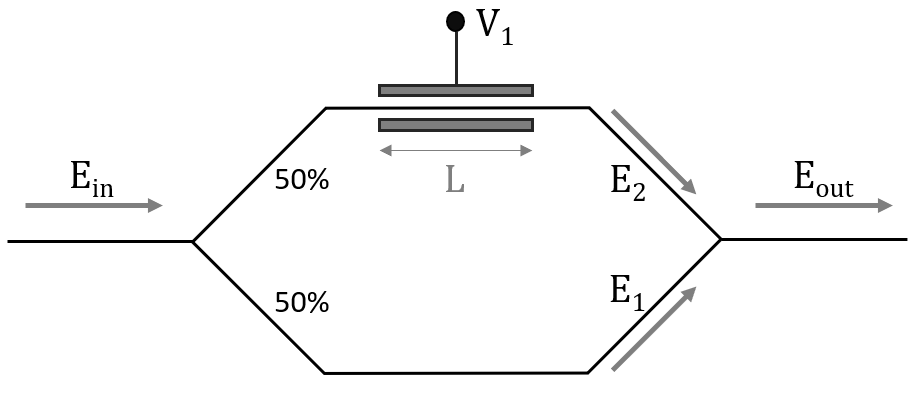
\includegraphics[width=0.7\columnwidth]{mach-zhen.png} 
\caption{Basic Mach-Zhedner modulator structure. An incoming optical signal is split equally into two paths of length $L$. The relative phase between these two paths is modulated. This is achieved by applying an electrical voltage $V_{1}$ to the propagation material (wave guide); changing the refractive index of one path. After phase modulation, the two optical paths are recombined and interference results in the modulation of the optical signal's intensity. Most Mach-Zhedner modulators will have electrodes on both arms, this figure depicts only one for conceptual simplicity.}
\label{fig-mach}
\end{figure}
\vspace{-0.5cm}
\begin{align*}
    E_{out} &= E_{1} + E_{2}\\
    &= \frac{E_0}{2}e^{ikL} + \frac{E_0}{2}e^{ikL + \Delta\phi} \\
    &\equiv 2\cos{\left(\frac{\Delta\phi}{2}\right)}\left(i\sin{\left(kL + \frac{\Delta\phi}{2}\right)}+\cos{\left(kL + \frac{\Delta\phi}{2}\right)}\right) \\
    &\propto cos{\left(\frac{\Delta\phi}{2}\right)}
\end{align*}
\begin{equation}
    \implies I_{out} \propto cos^2{\left(\frac{\Delta\phi}{2}\right)}
    \label{cos-squared-out}
\end{equation}
Eq. \ref{cos-squared-out} demonstrates that we should expect a sinusoidal-like output intensity with respect to applied voltage $V_1$, as $\Delta\phi$ varies between orders of $\pi$. 

'Bessel Tones' appear in the frequency domain if $V_1$ is sinusoidal about some bias with a frequency $f$:
\begin{align*}
    V_1 &= V_b + V_0\sin{(2\pi{}ft)}\\
    E_{out} &= \frac{E_0}{2}e^{ikL} + \frac{E_0}{2}e^{ikL + k_0 \Delta n(V_b + V_0\sin{(2\pi{}ft)})L}\\
\end{align*}
The optical carrier's phase modulation can then be described by
\begin{equation}
    \cos{(2\pi{}f_0t+V_0\sin{(2\pi{}ft)})}
    \notag
\end{equation}
according to \cite{freq}, where $f_0$ is the carrier frequency. This can be decomposed further into an infinite sum of 'Bessel Tones' which make up additional peaks in the optical spectrum.
\begin{figure}
\centering
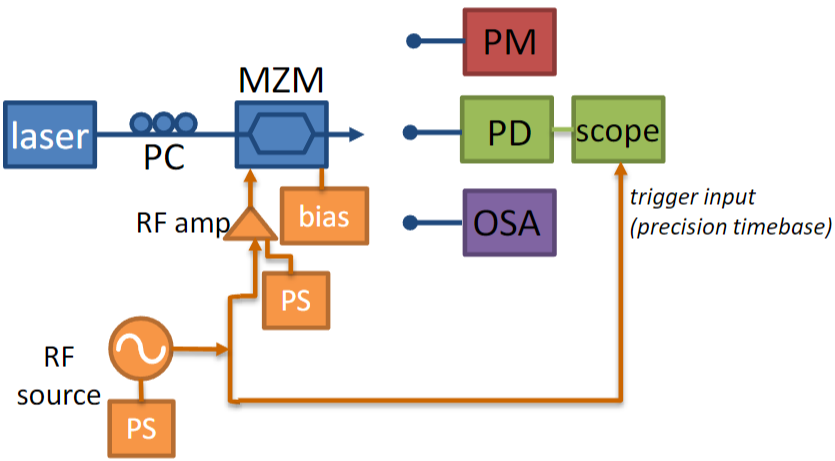
\includegraphics[width=0.7\columnwidth]{Fig-setup.png} 
\caption{Schematic representation of the utilised experimental setup. \cite{lab_brief}}
\label{fig-setup}
\end{figure}
\vspace{-0.5cm}
In the setup used throughout this report, A DFB (Distributed Feedback) laser is connected to a polarization controller (labelled PC in Fig \ref{fig-setup}), and subsequently to the Mach-Zehnder modulator (labelled MZM). The modulator output can then be connected to either a power meter for transfer function analysis or a patch cord (3dB splitter) for simultaneous optical spectrum and time domain response measurement with an Optical Spectrum Analyzer (OSA), photodetector (PD), and high-speed sampling scope. Importantly for modulation; A DC bias links to a power supply (PS), and an RF oscillator (RF source) feeds into an amplifier. 

\mychapter{2}{Initial Preparation}

It is important to be aware of some of the fundamental behaviour of devices independently; otherwise it may be difficult to draw conclusions, motivate their purpose, and make physical arguments later.

This section will focus on characterising the laser, polarisation controller and transfer function of the modulator.

\section{Laser Characterisation}
A basic characterisation of any laser diode includes an LI curve (light-current) and the spectrum of its output. A number of LI curves were taken in order to asses an average. This was done by connecting the laser's output directly to the power meter. The power meter can read out in dBm, which can be converted to mW using
\begin{equation}
    P_{mW}=10^{\frac{P_{dBm}}{10}}mW
\end{equation}
dBm is an absolute unit, unlike dB which is a relative ratio between two intensities. As such, the equivalent ratio between powers for a 3dB reduction in power can be found to be 50\%:
\begin{equation}
    P_{1}(dBm)-P_{2}(dBm)=10log_{10}\frac{P_{2}(mW)}{P_{1}(mW)}
    \notag{}
\end{equation}
if $P_2(mW) = \frac{P_1(mW)}{2}$:
\begin{equation}
    P_{1}(dBm)-P_{2}(dBm)=10log_{10}\frac{1}{2} = 10(-0.301) \approx -3dB
    \notag{}
\end{equation}
\begin{center}$\implies$ A 3dB reduction in power is a reduction of 50\%.\end{center}

Power fluctuations appeared significant and rapid during each measurement. It was concluded that there was possibility for systematic error between measurements - therefore 3 individual LI curve measurements were taken across 2 'runs' to produce 2 final measurements with error.

\begin{figure}
    \centering
    \subfloat[\centering Run 1]{{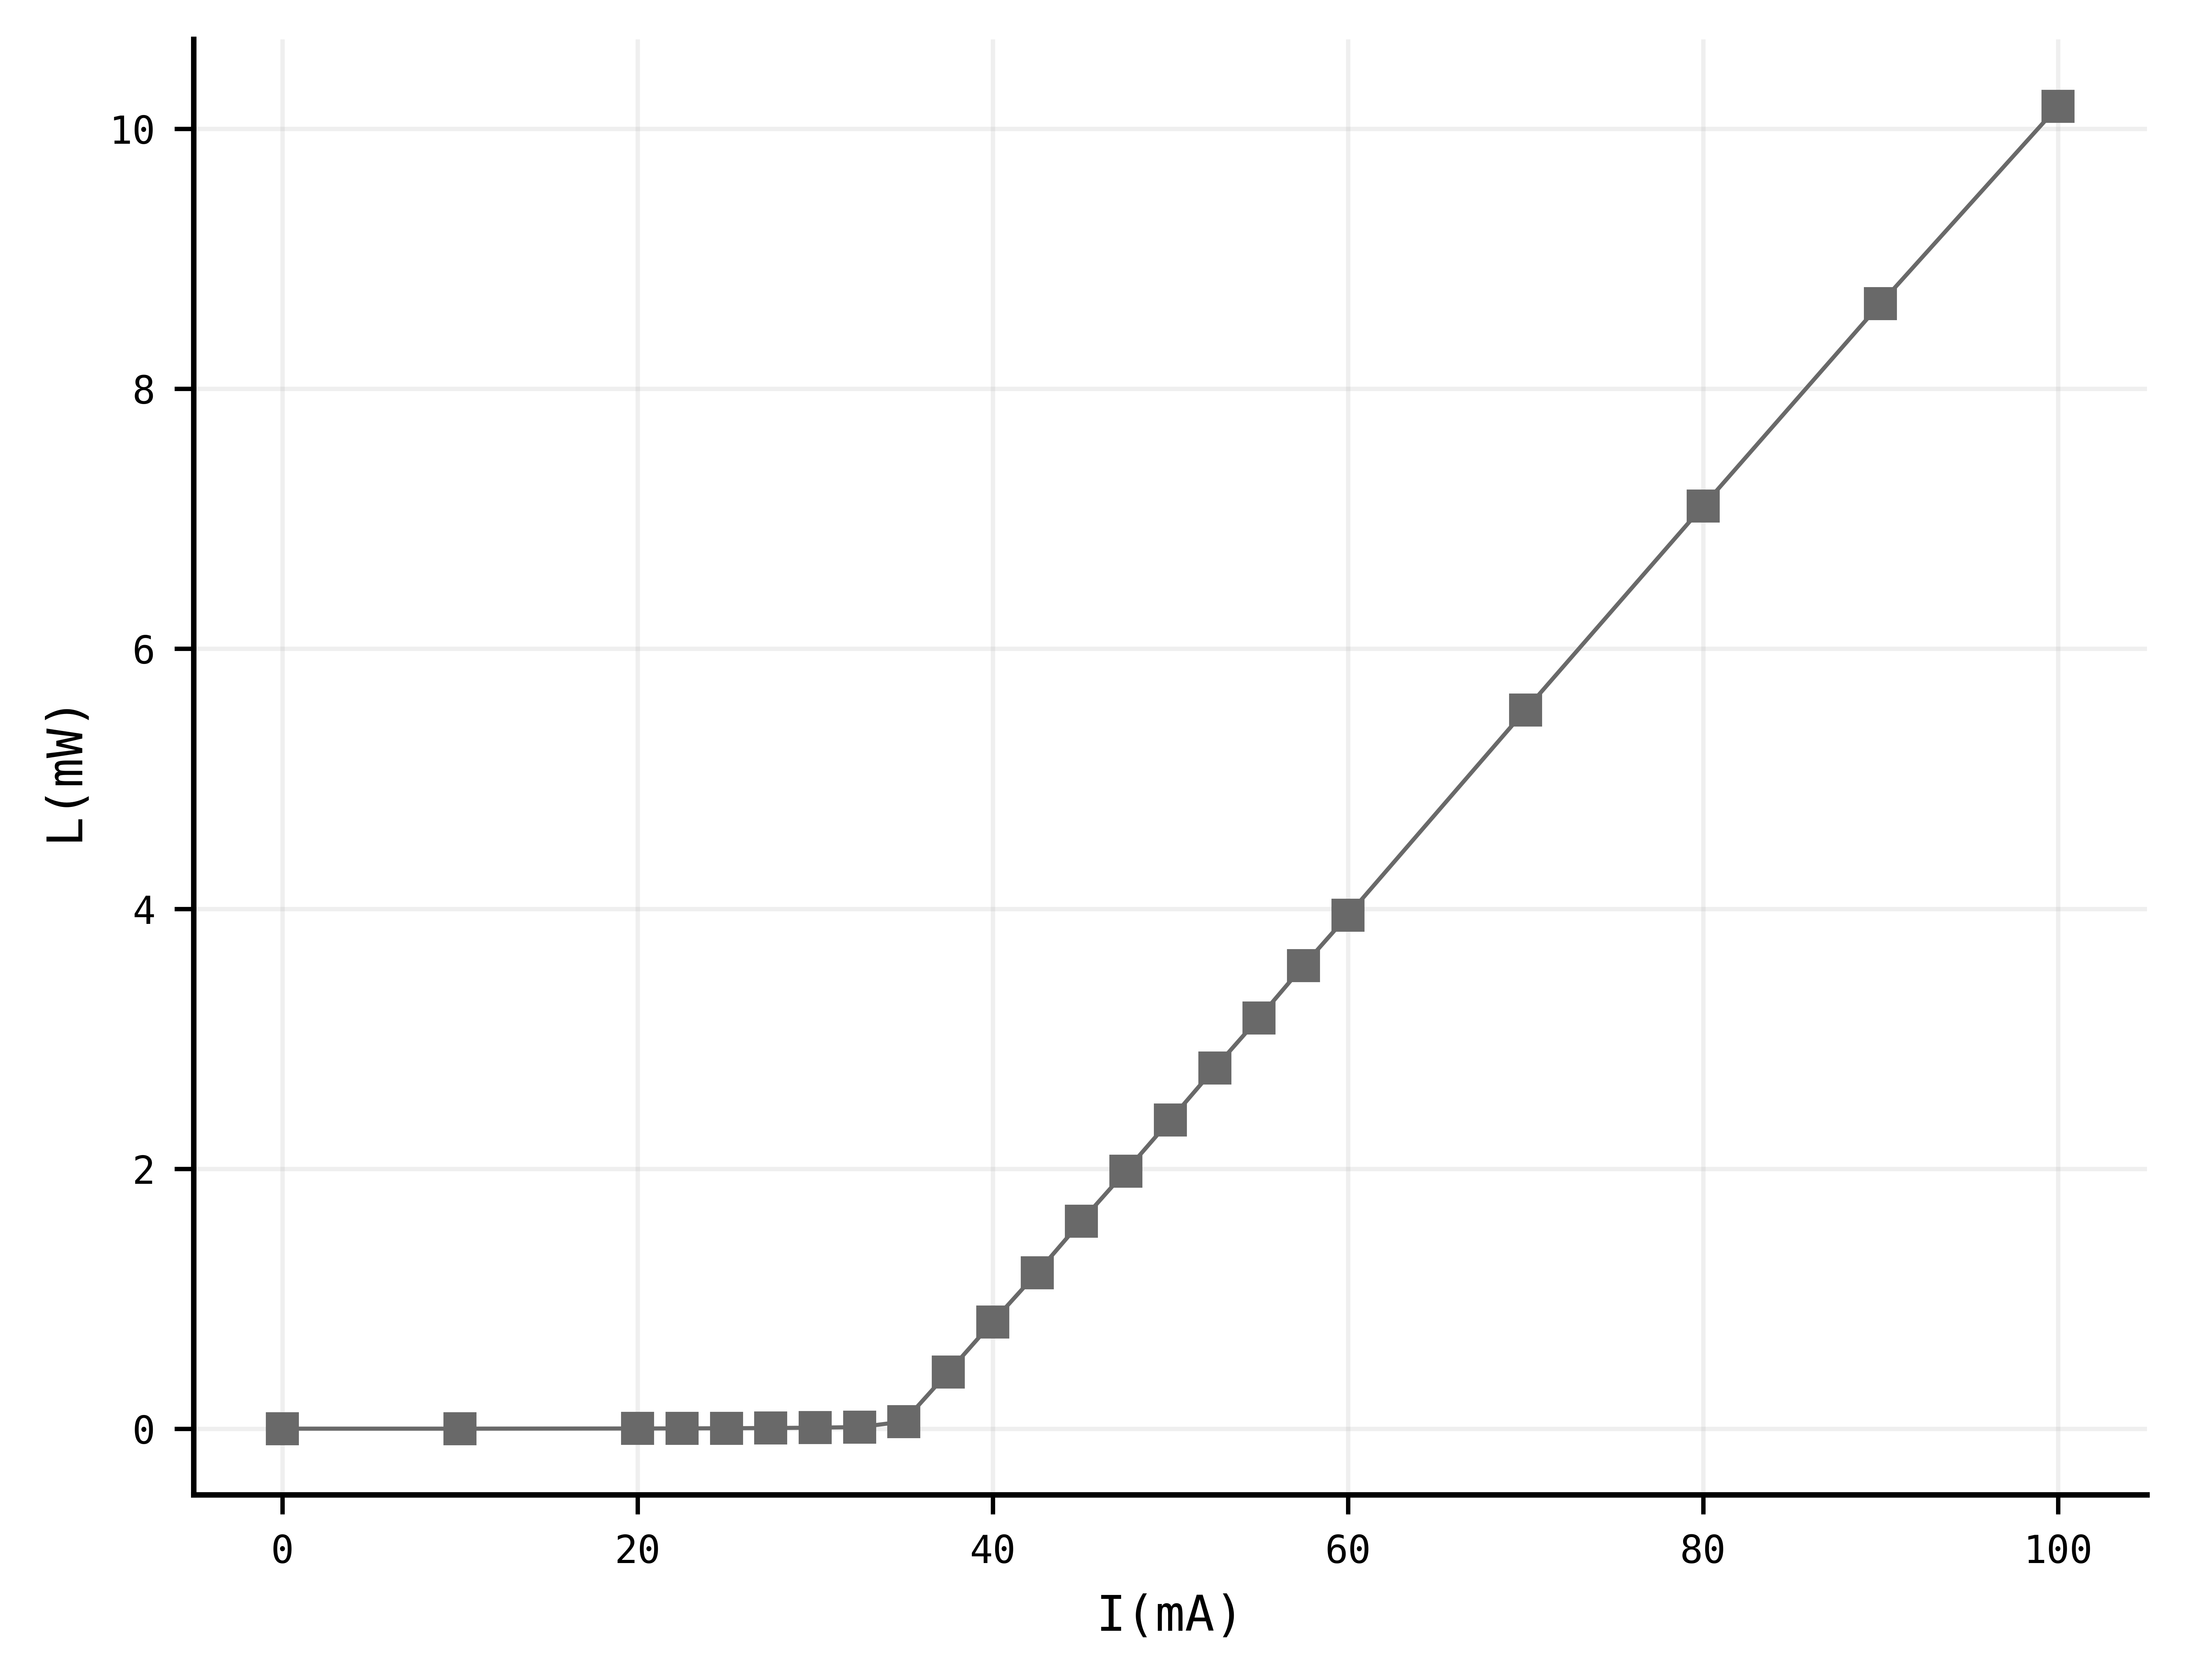
\includegraphics[width=0.475\columnwidth]{LI Curve Run 1 final_figure.png}}}%
    \quad
    \subfloat[\centering Run 2]{{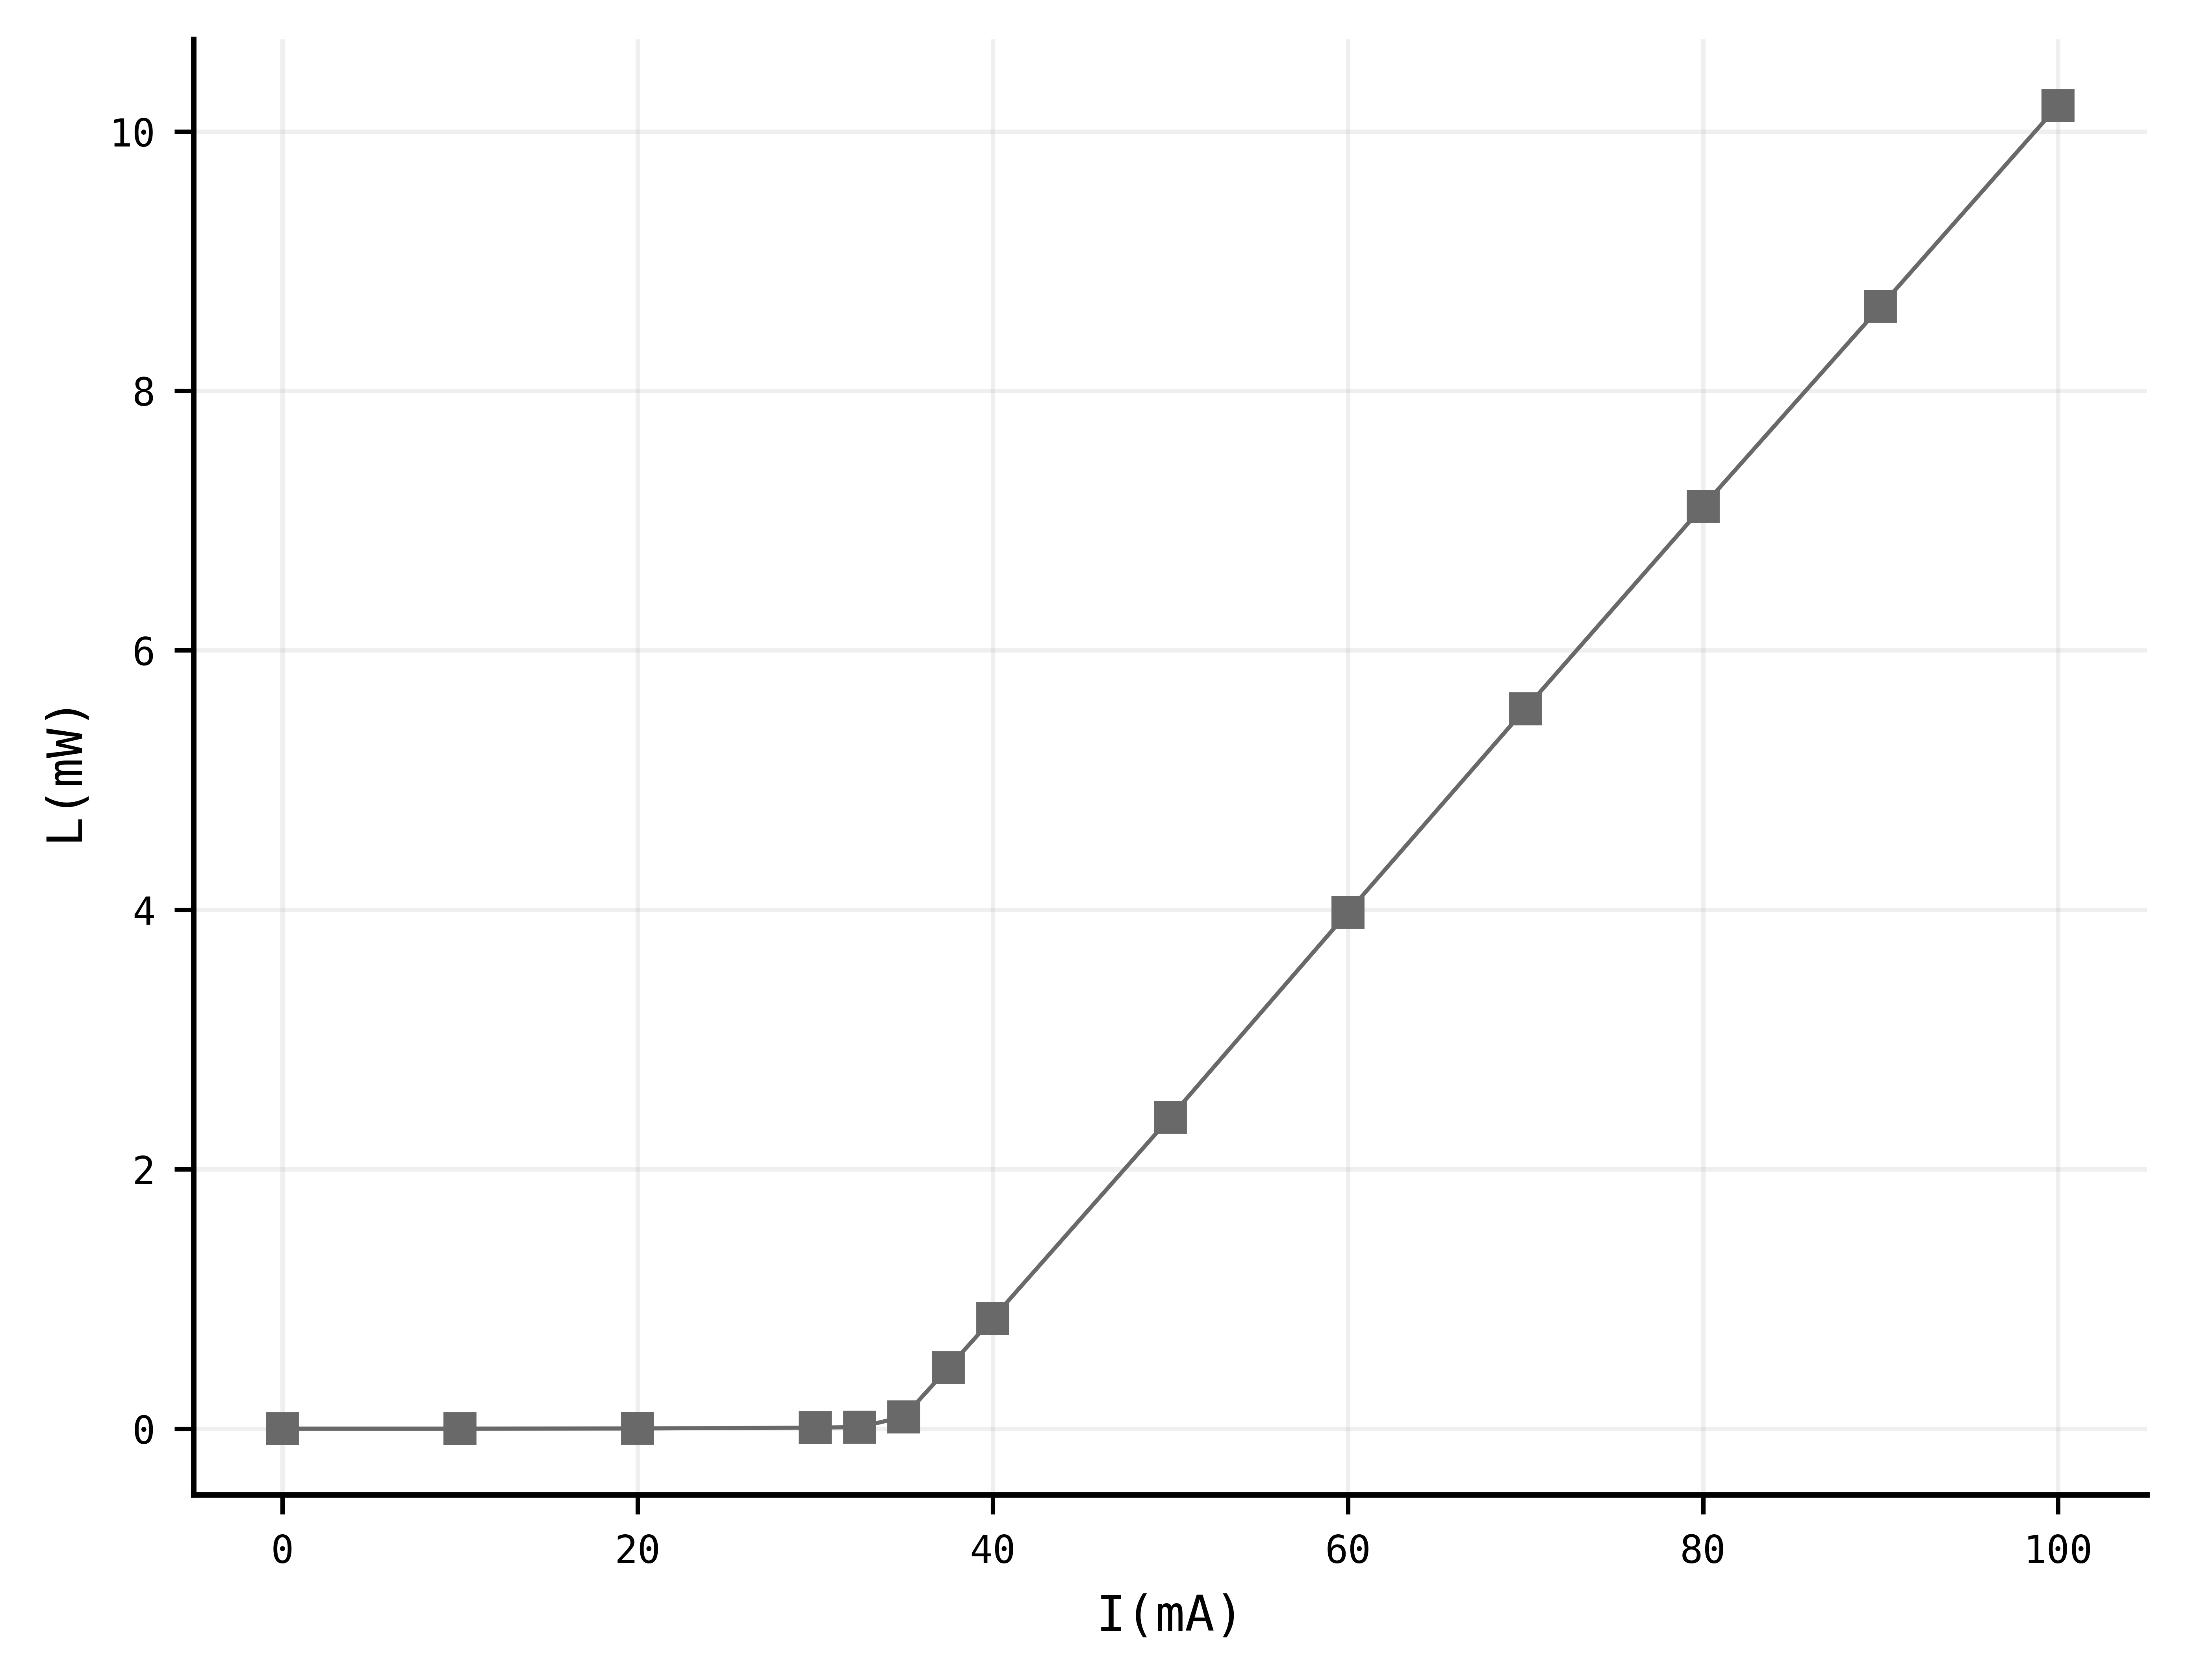
\includegraphics[width=0.475\columnwidth]{LI Curve Run II final_figure.png}}}
    \caption{LI Curves of the DFB laser at 25\degree{}C. Sub-figures \textbf{(a)} and \textbf{(b)} represent independent runs in which 3 measurements are averaged to create an LI curve with error bars. The error bars in both cases are plotted but negligible; the error between measurements at a set current in a particular run was typically less than 1\%. Data from \textbf{(a)} and \textbf{(b)} were recorded approximately an hour apart - no significant drift over time.}
    \label{fig LI curves}%
    \vspace{-12pt}
\end{figure}

The resulting LI curves are plotted in Fig \ref{fig LI curves}. The results were affected less by measurement fluctuations than expected - this effort was an overcompensation brought on by the power meter's display changing between orders of units. Regardless, it shows the laser output remained consistent at 25°C. Using interpolation in Excel, we derived power-current equations from Run 1 and Run 2 data:
\begin{align*}
    L_1 [mW] &= 0.1564 I_1 - 5.4331 \\
    L_2 [mW] &= 0.1555 I_2 - 5.3586
\end{align*}
where $I_1$,$I_2$ is in $mA$. Averaging these we conclude with confidence
\begin{equation}
    L_{laser} [mW] = 0.1559 I_{source} - 5.3959 \\
    \label{L_laser}
\end{equation}
with $I_{source}$ in $mA$. We will use Eq. \ref{L_laser} later to set the laser to 10dBm/10mW.

From Fig \ref{fig LI curves} lasing threshold is apparent at approximately 35mA. Using Eq \ref{L_laser} we can verify this further:

\begin{align*}
    L_{laser} [mW] \approx 0 &= 0.1559 I_{threshold} - 5.3959 \\
    \implies I_{threshold} &\approx 34.6113 mA 
\end{align*}

Fig \ref{fig-temp-laser} demonstrates that device temperature has a significant impact on the output and validates the necessity of the temperature controller in the setup. 

\begin{figure}
\centering
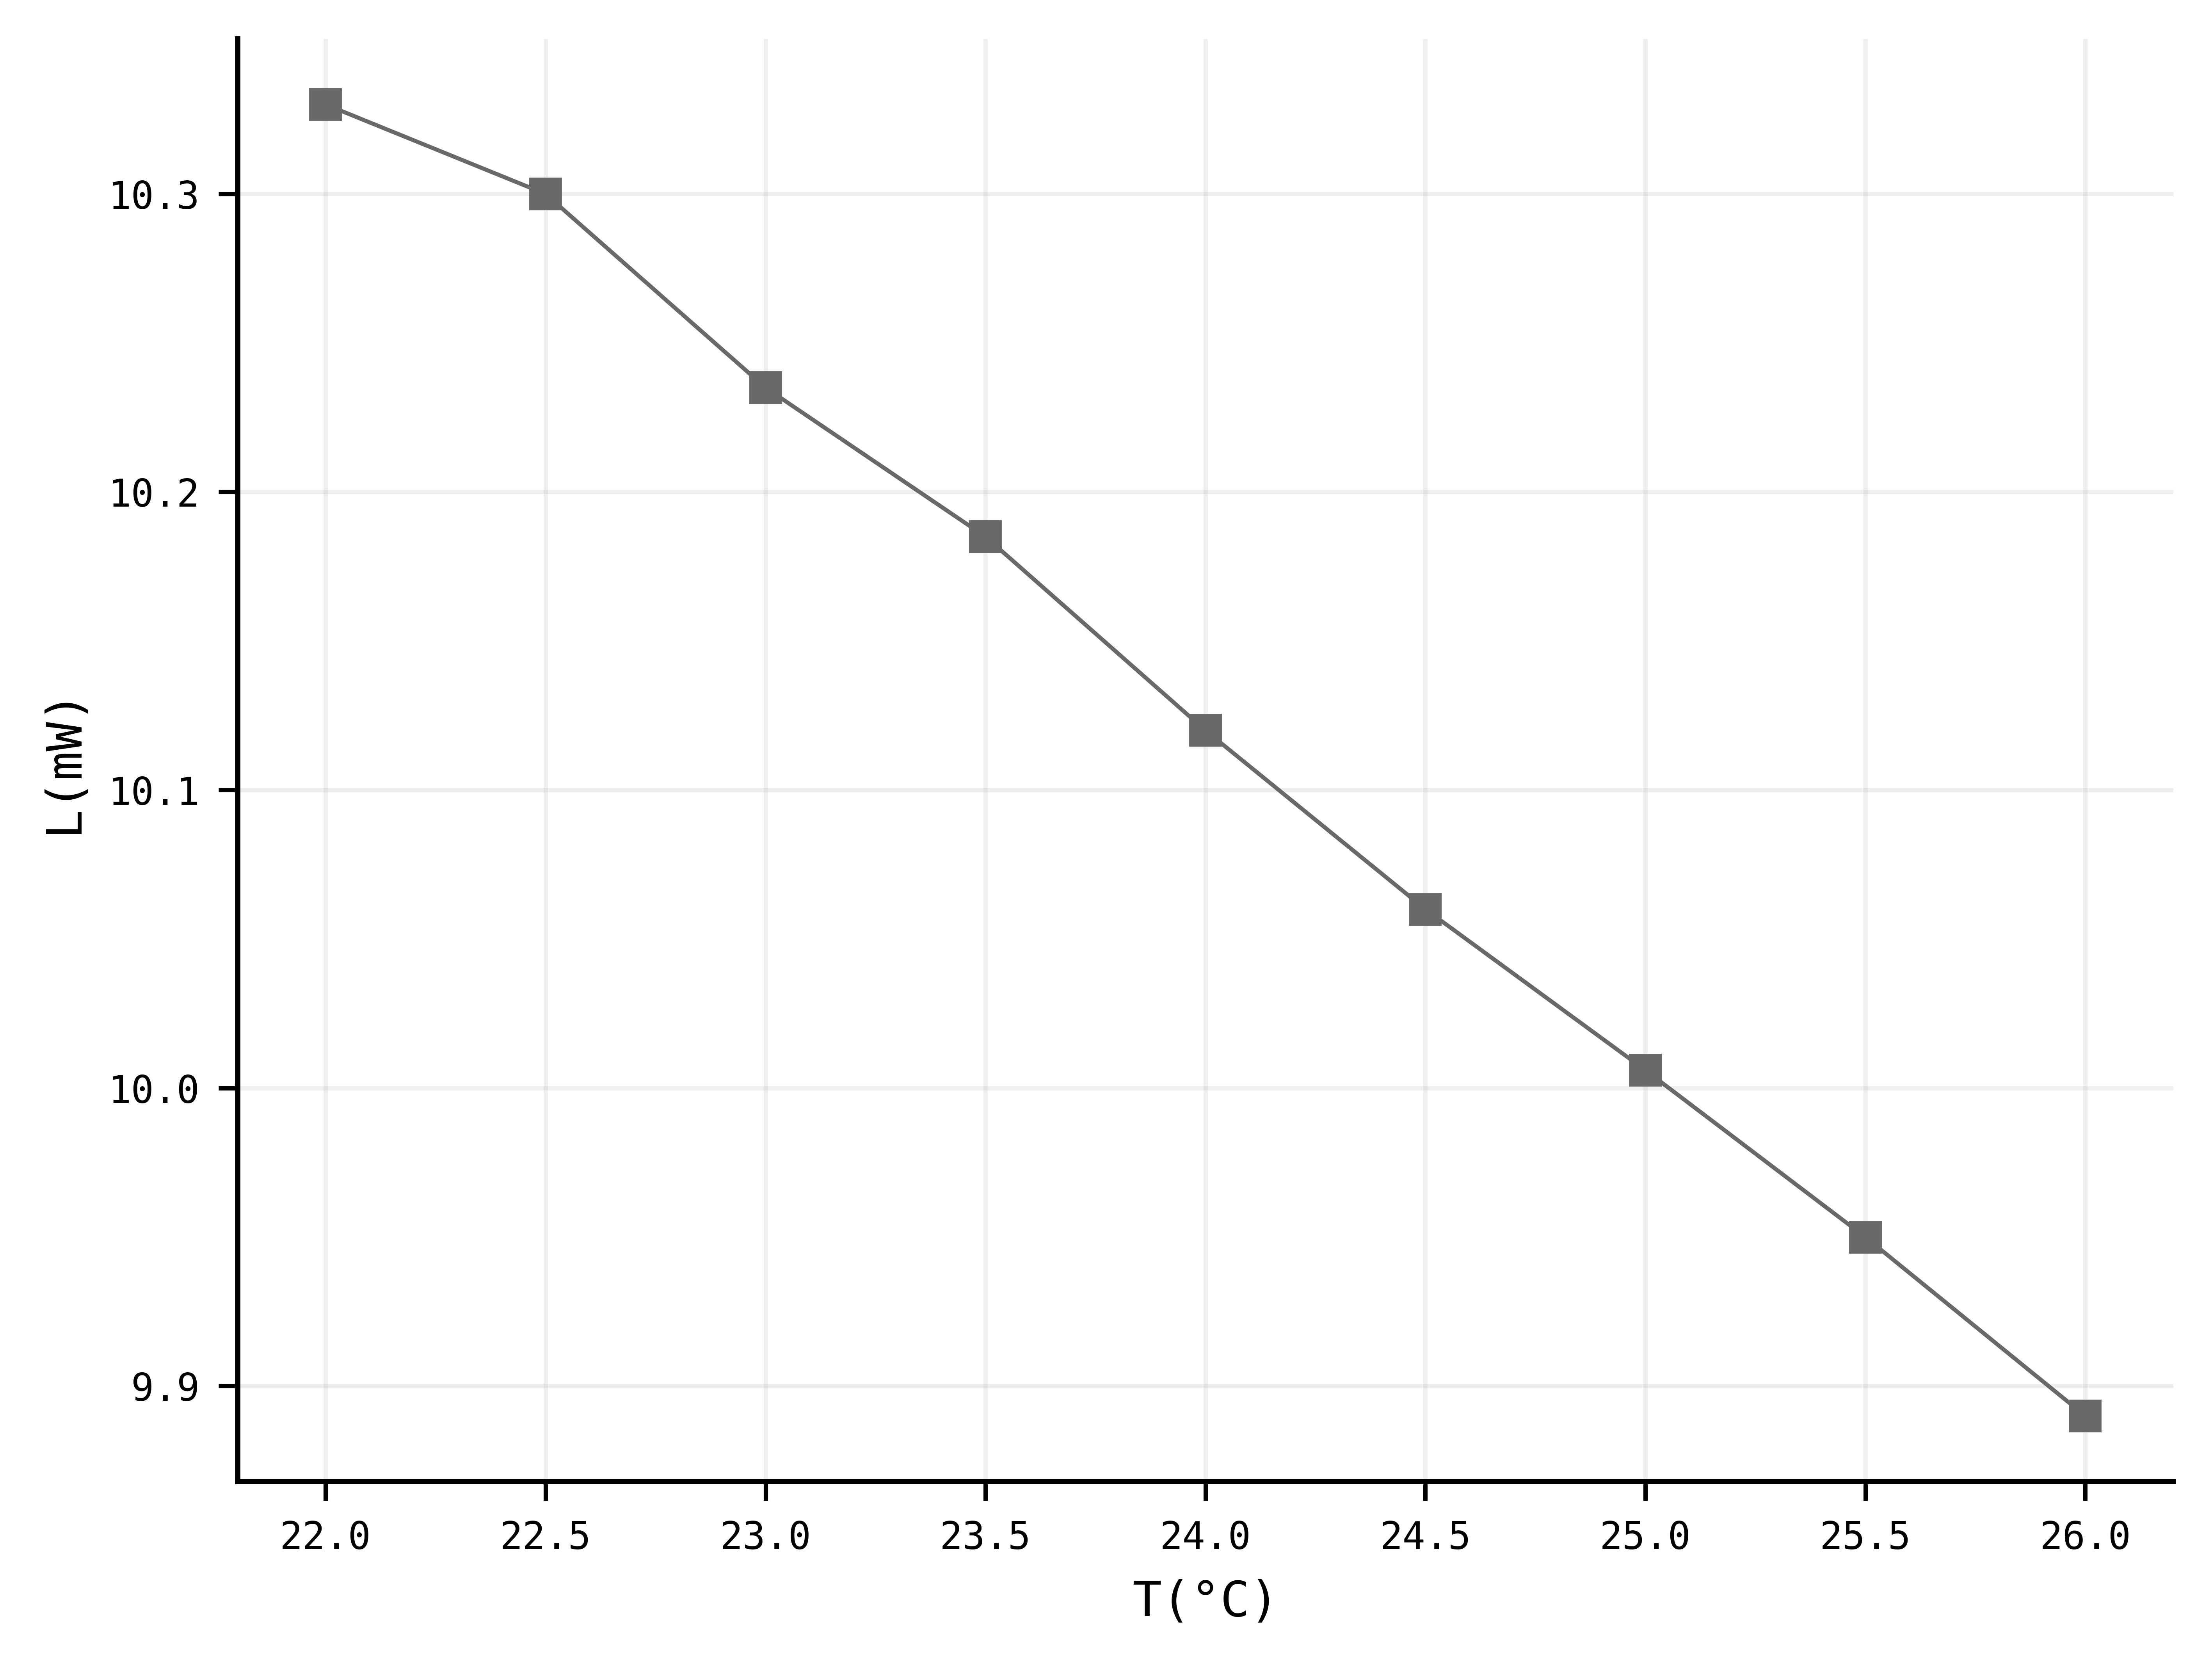
\includegraphics[width=0.7\columnwidth]{LvsT10mWfinal_figure.png} 
\caption{DFB laser output at 98.9mA with respect to temperature. Temperature was controlled using the temperature controller that the laser is mounted to. As temperature increases, the laser's output decreases - the laser becomes less efficient. This demonstrates the purpose and necessity of the temperature controller's presence in the setup.}
\label{fig-temp-laser}
\end{figure}
\vspace{-0.5cm}
The minimum safe operating distance of the laser beam (coming out of the fibre tip) can be calculated using the 'Nominal-Ocular Hazard Distance' (NOHD) formula \cite{ucclaser}:
\begin{equation}
    NOHD=2\sqrt{\frac{P}{MPE\pi\theta^2}}
    \notag
\end{equation}
Where $MPE$ is Maximum Permissible Exposure, $\theta$ is beam divergence and $P$ is optical power. For a singlemode optical fibre and assuming a Gaussian beam profile, \cite{ucclaser} tells us that 
\begin{equation}
    d_{63}=z\theta=\frac{2\sqrt{2}z\lambda}{\pi\omega_{0}}
    \notag
\end{equation}
where $d_{63}$ is an aperture which \textit{"would pass 63.2\% of the total intensity"}\textsuperscript{\cite{ucclaser-tables}}. From this we can calculate
\begin{equation}
    \theta=\frac{2\sqrt{2}\lambda}{\pi\omega_{0}}=\frac{2\sqrt{2}(1550\times 10^{-9})\text{ m}}{\pi (10\times10^{-6}\text{ m})}=0.1395 \text{ rad}
    \notag
\end{equation}
According to \cite{ucclaser-tables}, the effective accidental ocular exposure time of a 1550nm laser is $>100s$ with a corresponding $MPE = 1000Wm^{-2}$ from Tab A.1\textsuperscript{\cite{ucclaser-tables}}.
$P = 10mW$ will be the maximum power used throughout experiment.
\begin{equation}
    NOHD=2\sqrt{\frac{10mW}{1000Wm^{-2}\pi(0.1395)^2}}=2.56cm
    \notag
\end{equation}

Next, The lasers optical spectrum was measured and analysed under various changing conditions. Fig \ref{OSA} shows scans of the OSA's external monitor with the temperature controller set to different temperatures.

\begin{figure}
    \centering
    \subfloat[\centering 25\degree{}C]{{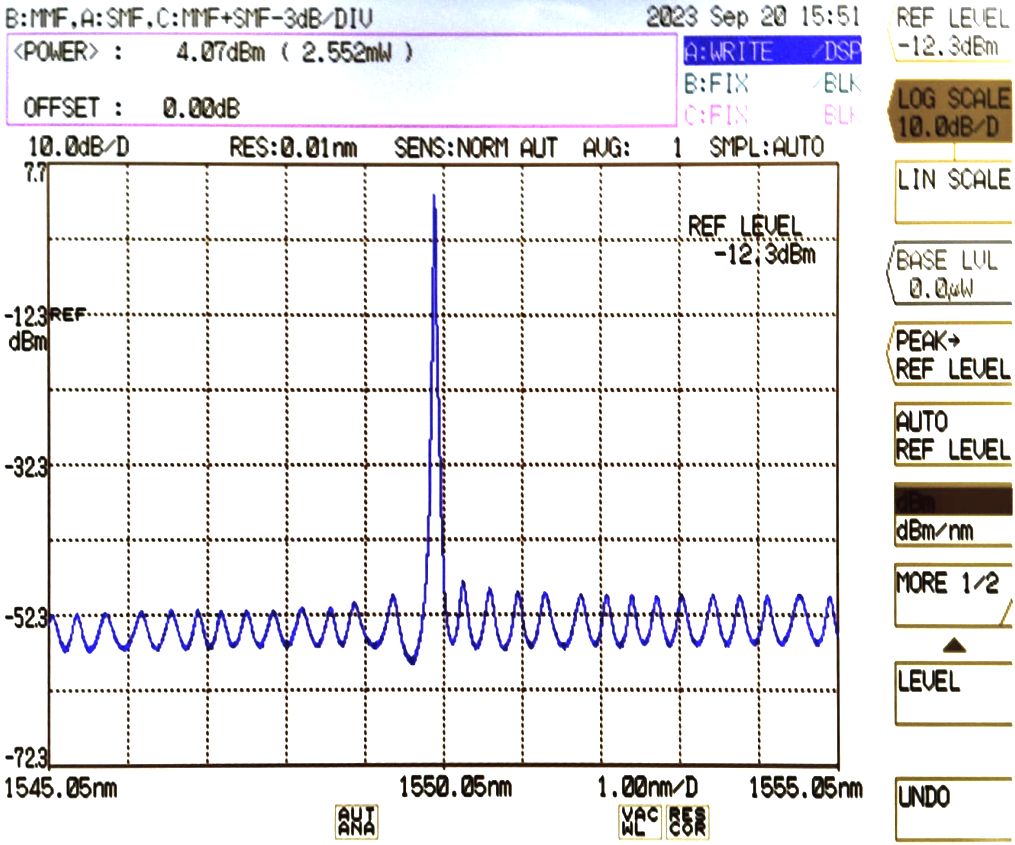
\includegraphics[width=0.475\columnwidth]{OSA_laser1.png}}}%
    \quad
    \subfloat[\centering 24\degree{}C]{{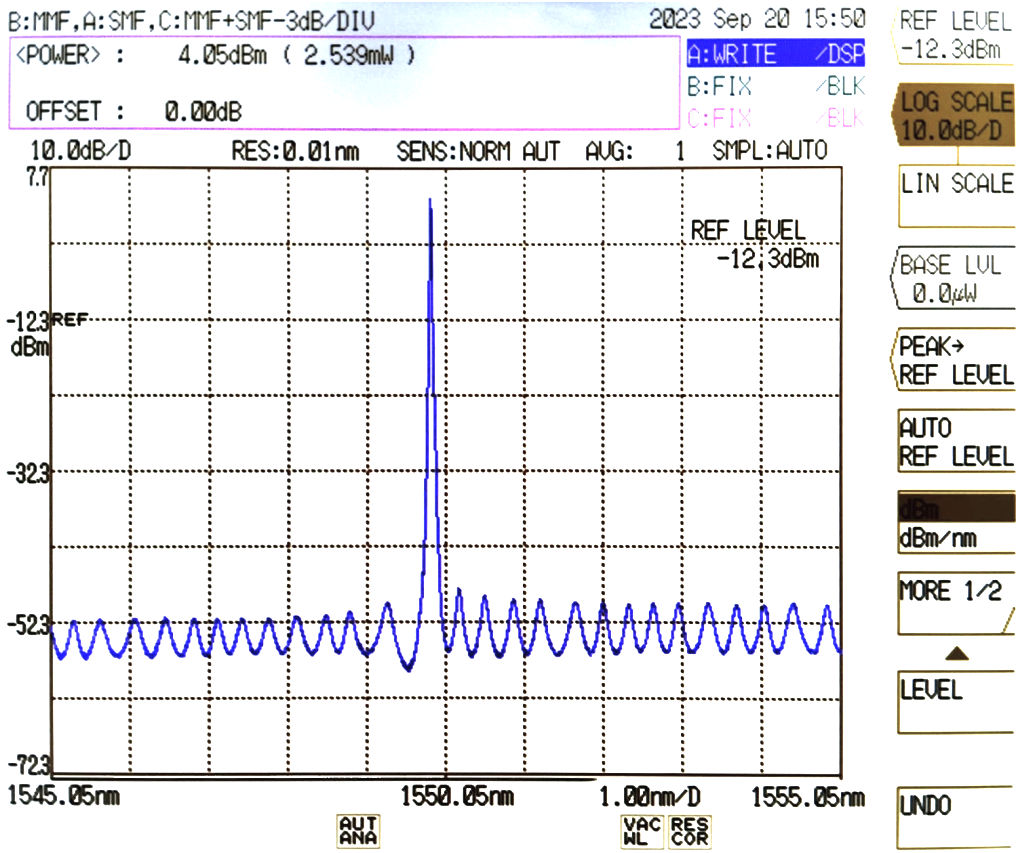
\includegraphics[width=0.475\columnwidth]{OSA_laser2.png}}}
    \quad
    \subfloat[\centering 23\degree{}C]{{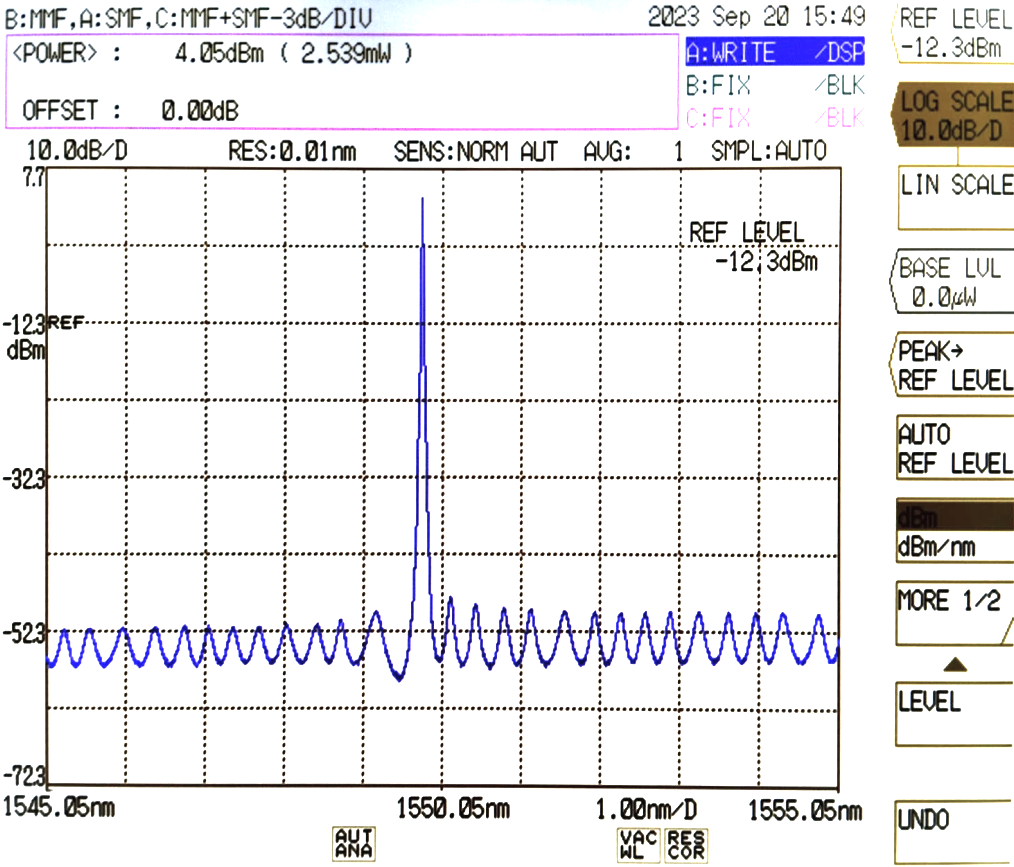
\includegraphics[width=0.475\columnwidth]{OSA_laser3.png}}}%
    \quad
    \subfloat[\centering 22\degree{}C]{{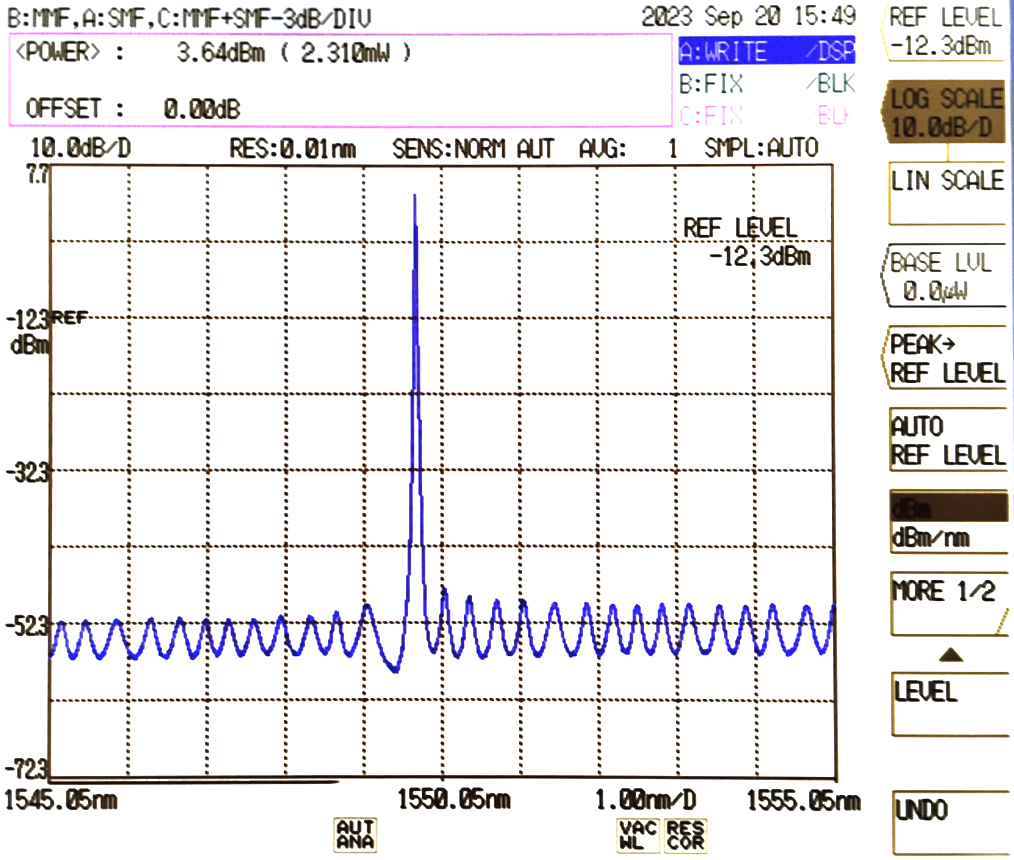
\includegraphics[width=0.475\columnwidth]{OSA_laser4.png}}}%
    \caption{OSA spectrums of the laser at various temperatures. The labels on each sub-figure represent the temperature at which the device was kept, set by the temperature controller. There is a noticeable trend of shifting peak wavelength with respect to temperature. An estimation of the specific wavelength shifts have been demonstrated in Tab \ref{OSA-t}.}
    \label{OSA}%
    \vspace{-12pt}
\end{figure}
\begin{table}[htbp]
  \centering
  \label{tab:sample-table}
  \begin{tabular}{rrrrr}
\toprule
   \textbf{T (\degree{}C)} &   \textbf{1550.05nm (px)} &   \textbf{1545.05nm (px)} &   \textbf{Spectrum peak (px)} &   \textbf{$\lambda_T$ (nm)} \\
\midrule
                22 &                       441 &                        50 &                           415 &                     1549.72 \\
                23 &                       442 &                        46 &                           421 &                     1549.78 \\
                24 &                       445 &                        50 &                           430 &                     1549.86 \\
                25 &                       444 &                        48 &                           433 &                     1549.91 \\
\bottomrule
\end{tabular}
  \caption{Further demonstration of specific wavelength changes with respect to operating temperatures. $\lambda_T$ is the calculated operating wavelength for a temperature $T$, this was calculated using the horizontal pixel number of grid lines/markers in the OSA scans (Fig \ref{OSA}). See \ref{A.1} for the specific formula used to calculate $\lambda_T$.}
\label{OSA-t}
\end{table}

Fig \ref{OSA} and Tab \ref{OSA-t} demonstrate the temperature dependence of the peak wavelength, which is a well known and documented characteristic of semi-conductor lasers \cite{temp-dependance1}. Tab \ref{OSA-t} shows a roughly linear relationship, where $\frac{d\lambda_{peak}}{dT} \approx 0.06nm$. \cite{temp-dependance2} cites two main contributors to have an effect on the crystal band structure of the laser: \textit{"thermal lattice expansion, associated with the dependence of the carrier energy levels on the unit cell volume, and electron-phonon interaction"} with reference to \cite{temp-dependance3}, \cite{temp-dependance4}. That is; the semi-conductor is physically changing shape, effecting the band-gap (and subsequently emission wavelength).

The current dependence was also investigated. Fig \ref{OSA-current} demonstrates the spectrum about lasing threshold, $I_{threshold} \approx 35mA$.

\textit{\textbf{Note to marker:} it was not possible to export the OSA data, therefore we cannot answer question \textbf{3. g(i)} of the lab brief fully.}

If we had been able to export the OSA data, it would have been possible to approximate the carrier/junction temperature of the laser by fitting a boltzmann distribution to the high energy wing of the energy spectrum \cite{energy}. \emph{(This was something that had been intended to do - code had been prepared which is included in \ref{code} with example output)}

\begin{figure}
    \centering
    \subfloat[\centering 27.5mA]{{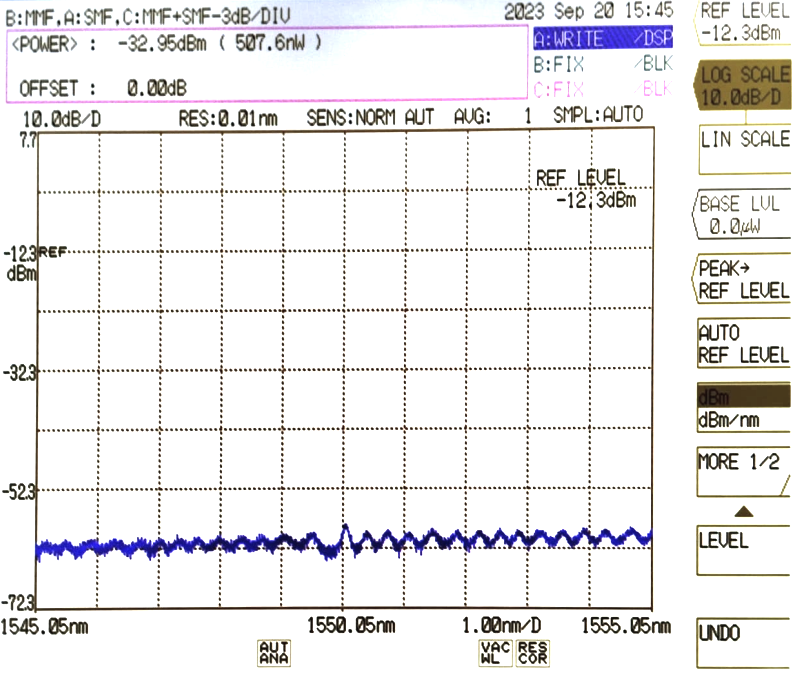
\includegraphics[width=0.475\columnwidth]{OSA_current27.5mA.png}}}%
    \quad
    \subfloat[\centering 30mA]{{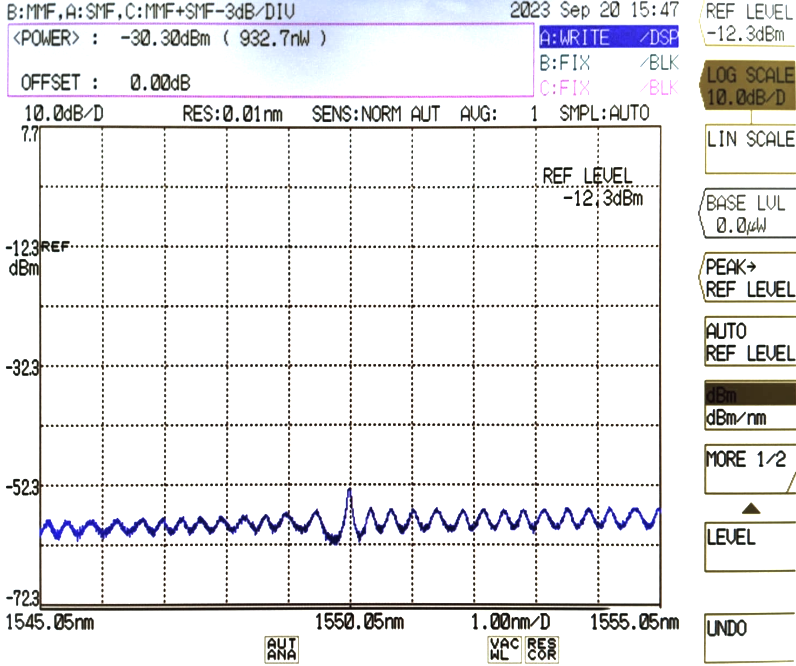
\includegraphics[width=0.475\columnwidth]{OSA_current30mA.png}}}
    \quad
    \subfloat[\centering 32.5mA]{{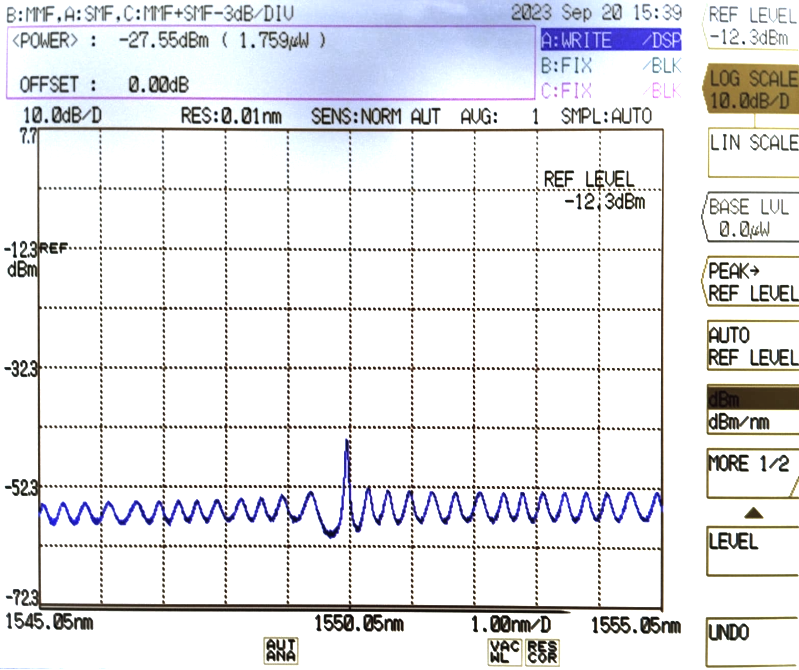
\includegraphics[width=0.475\columnwidth]{OSA_current32.5mA.png}}}%
    \quad
    \subfloat[\centering 37.5mA]{{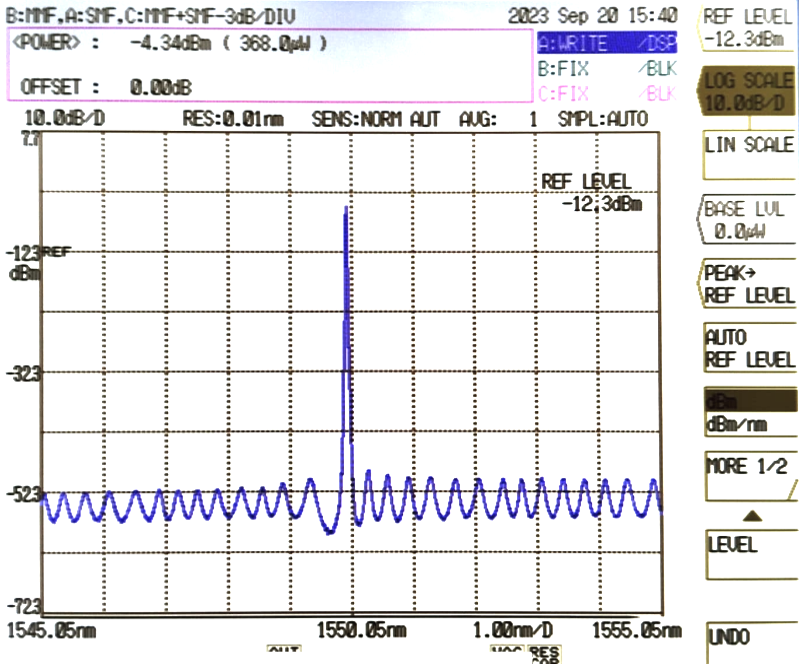
\includegraphics[width=0.475\columnwidth]{OSA_current37.5mA.png}}}%
    \caption{OSA measurements about lasing threshold at 25\degree{}C. There is a small shift in peak wavelength as the current approaches the previously determined lasing threshold. The periodicity of the intensity with respect to frequency visible in all sub-figures is a common feature of DFB lasers, example \cite{laser1}.}
    \label{OSA-current}
    \vspace{-12pt}
\end{figure}

\section{Polarisation Controller}
As shown in Tab \ref{PC-loss}, the insertion loss of the polarisation controller was measured to be $0.25$dB.

\begin{table}[htbp]
  \centering
  \label{tab:sample-table}
  \begin{tabular}{rrrr}
\toprule
   \textbf{Max. (dBm)} &   \textbf{Min. (dBm)} &   \textbf{Avg. (dBm)} &   \textbf{Loss (dB)} \\
\midrule
                  9.78 &                  9.74 &                  9.75 &                  0.25 \\
\bottomrule
\end{tabular}
  \caption{Insertion loss measurements. The laser is operated at 10dBm according to eq. \ref{L_laser}. Maximum and minimum values for power were determined by varying the 'bat-ears' of the polarisation-controller and reading from the power meter. The average insertion loss was determined by converting dBm measurements to mW, averaging the max/min, and converting back to dBm. Therefore, there is an effective insertion loss of 0.25dB.}
    \label{PC-loss}
\end{table}
This result was to be expected. A polarization controller physically adjusts the polarization state of light by rotating or modifying the orientation of its electric field - it does not filter light based on its polarisation or break it down into subsequent components (this would reduce it's intensity). Also, the power-meter is \textit{not} polarisation dependant, so the measured insertion loss is accurate and minimal.
\section{Characterisation of Loss and Polarisation Extinction Ratio of the Modulator}
\begin{table}[htbp]
  \centering
  \label{tab:sample-table}
  \begin{tabular}{rrrr}
\toprule
   \textbf{Max. (dBm)} &   \textbf{Min. (dBm)} &   \textbf{Loss (dB)} &   \textbf{Polarisation Extinction Ratio (dB)} \\
\midrule
                  2.79 &               -15.407 &                  7.21 &                            18.197 \\
\bottomrule
\end{tabular}
  \caption{Recorded Insertion loss and polarisation extinction ratio of the Mach Zehnder modulator. Here, the laser was set to an intensity of 10dBm using \ref{L_laser} and upon instruction of supervisor the bias voltage of the modulator set to 5.4V. Maximum and minimum values for power were determined by varying the ’bat-ears’ of the polarisation-controller and reading from the power meter.}
  \label{loss-ext}
\end{table}
As shown in Tab \ref{loss-ext} the insertion loss of the modulator was recorded to be 7.21dB. The polarisation extinction ratio (PER) was determined to be ($2.79$dBm+$15.407$dBm) = $18.197$dB. According to the spec sheet of the modulator \cite{modulator-spec}, we should expect a "DC Extinction Ratio" of $\geq 20$dB \textsuperscript{\cite{modulator-spec}} and an insertion loss of $3.2$dB\textsuperscript{\cite{modulator-spec}}.

We are not told \emph{explicitly} what the 'polarisation extinction ratio' of the modulator is in \cite{modulator-spec}, however typical PER's of $20$dB have been specifed for LiNbO$_{3}$ modulators \cite{PER}. Our insertion loss measurement is significantly larger than the spec sheet. Both of these results are likely due to unaccounted loss or polarisation within the optical fibres of the setup. Simply varying the orientation of the 'bat-ears' may not have been enough to infer the actual maximum intensity. In a loose optical fibre "non-uniform stresses"\textsuperscript{\cite{PER}} may be introduced by bends or movement resulting in additional birefringence. A dirty fibre tip may have also caused losses.

\section{Modulator Transfer Function}\label{sec:TF}
\begin{figure}
\centering
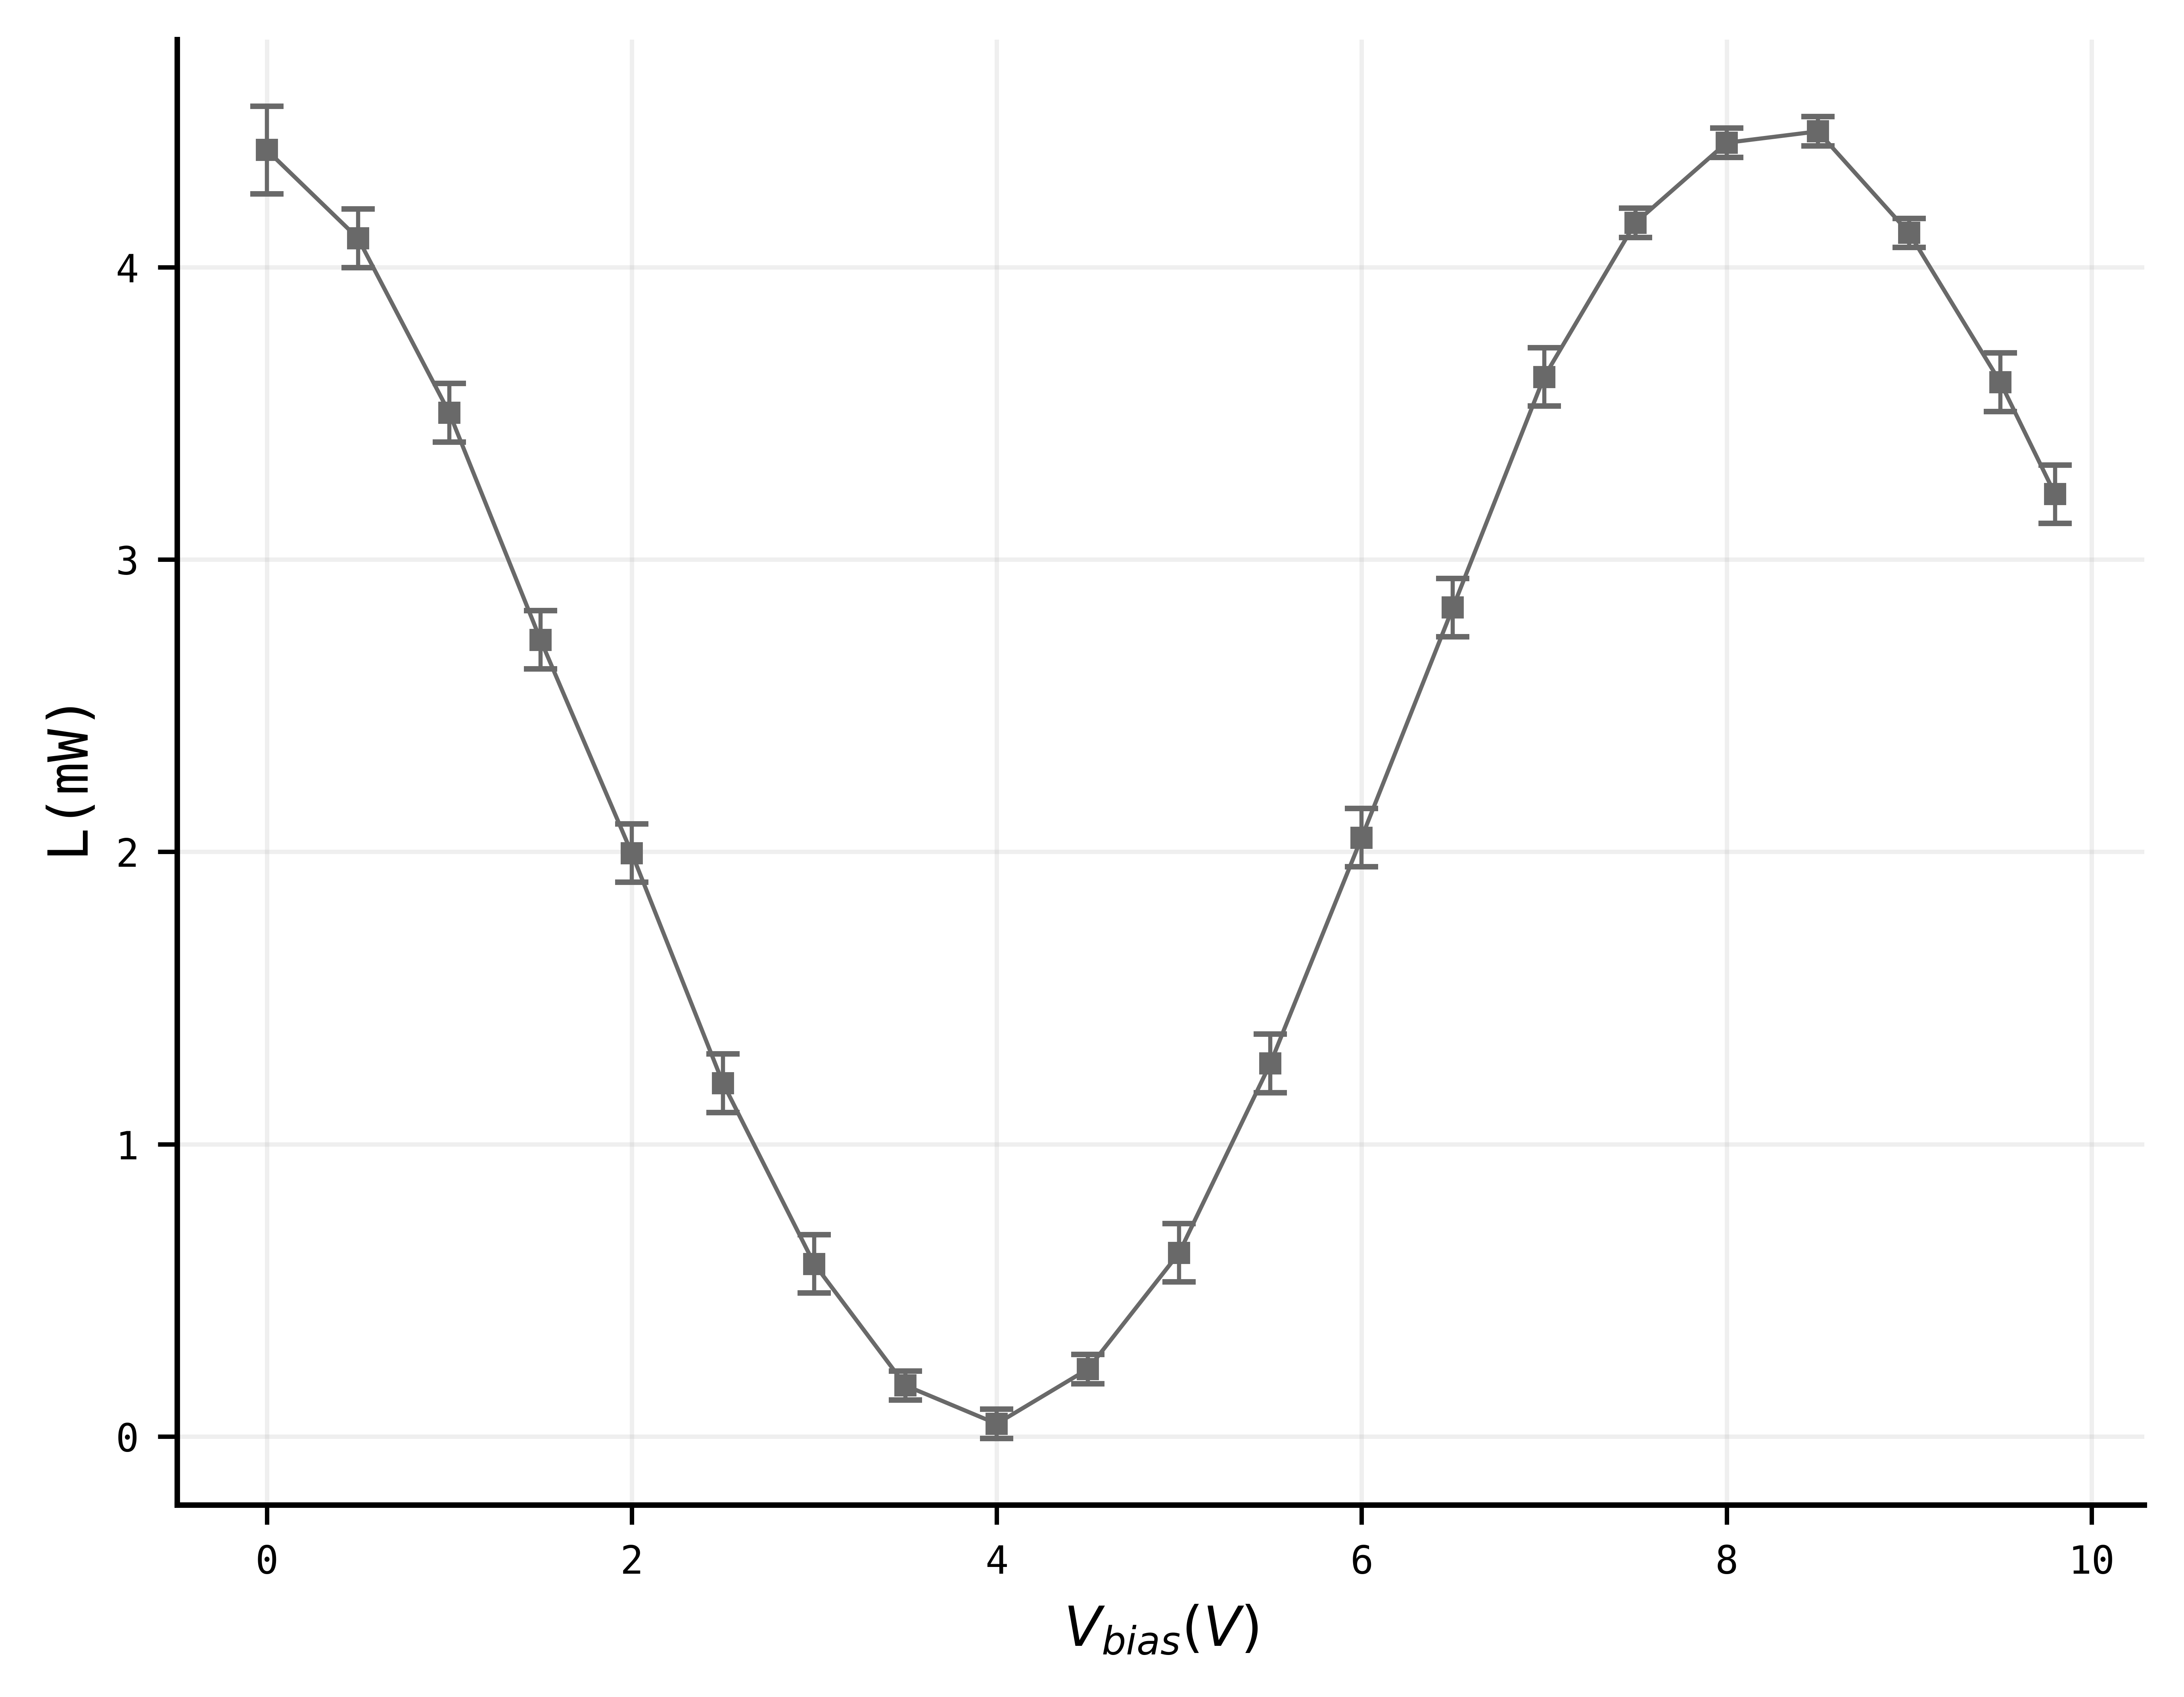
\includegraphics[width=0.85\columnwidth]{Transfer Function 1(mW)error_figure.png} 
\caption{Plotted transfer function of the modulator at the maximum polarisation setting. Error bars shown represent consistent fluctuation of approximately $\pm{}$0.1mW, except at the minimum/maximum where this fluctuation was present but much less noticeable. At zero volts the output was more unstable than any other point.}
\label{fig-transfer1}
\end{figure}
A recorded transfer function is shown in Fig \ref{fig-transfer1}. It is a sinusoidal shape, which we would expect analogous to Eq. \ref{cos-squared-out}. As discussed in 'fundamentals', The phase of the laser light is altered by applying a voltage to the wave guides within the modulator which changes it's refractive index. Since interference is phase dependant and the phase difference is periodic with respect to refractive index, we expect a sinusoidal-like transfer function with respect to bias. The error bars in Fig \ref{fig-transfer1} represent the degree of fluctuation present at the time of measurement, however these are not a full scope of error. Multiple transfer functions were plotted; the function was found to drift over time. See Figures \ref{fig-transfer2}, \ref{fig-transfer3}.

From the combined findings of Figures \ref{fig-transfer1}, \ref{fig-transfer2}, \ref{fig-transfer3} we are going to imply an effective quadrature point at $5.4/5.5$V to account for the transfer function drift over time.

\begin{equation}
    V_{\pi} \approx 6\text{V}
    \label{quadpoint}
\end{equation}

This is close to the bias voltage specified by the spec sheet, \cite{modulator-spec}. The other critical points of relevance (accounting for drift) are:
\begin{align*}
    V_{max} &\approx 8.5\text{V}\\
    V_{min} &\approx 4\text{V}
\end{align*}

\begin{figure}
\centering
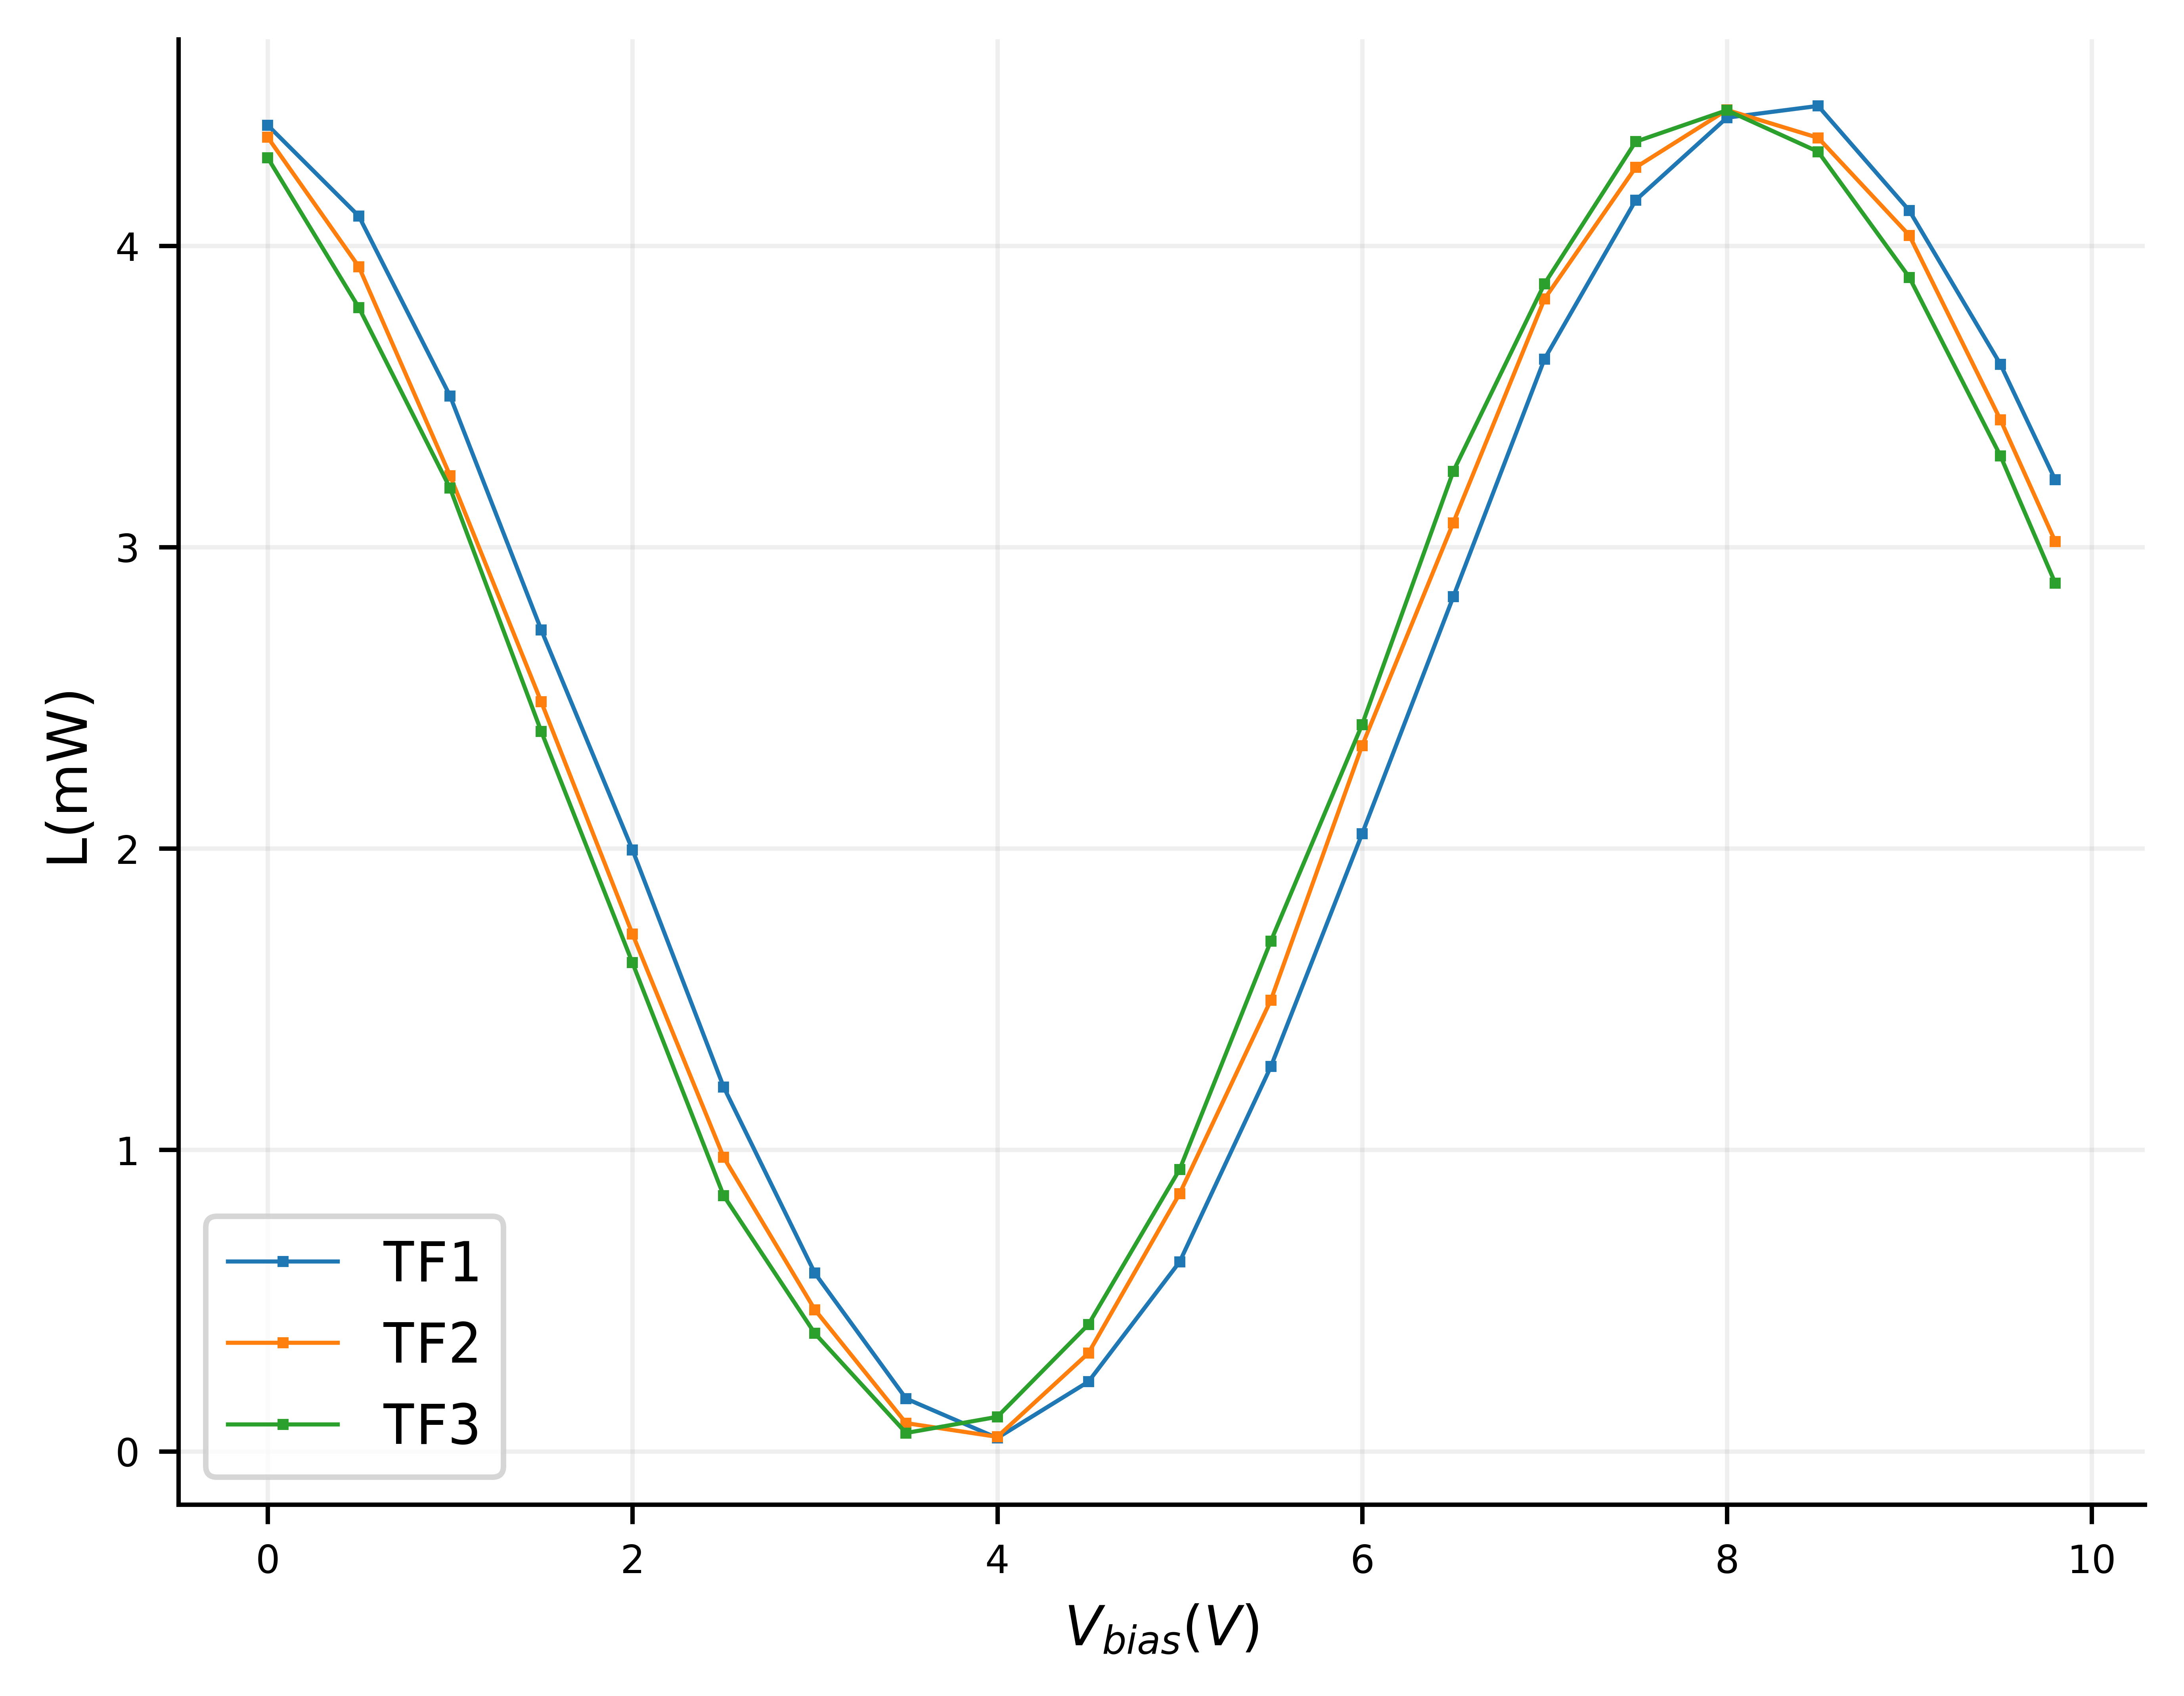
\includegraphics[width=0.85\columnwidth]{Transfer Function 3(mW)_figure_all.png} 
\caption{Plotted transfer functions of the modulator at the maximum polarisation setting. Here 'TF1', 'TF2', and 'TF3' represent sequentially recorded transfer functions over the course of approximately an hour. The transfer function drift is clearly visible.}
\label{fig-transfer2}
\end{figure}

\begin{figure}
    \centering
    \subfloat[\centering $V_{bias} \approx V_\pi \approx 5.5V$]{{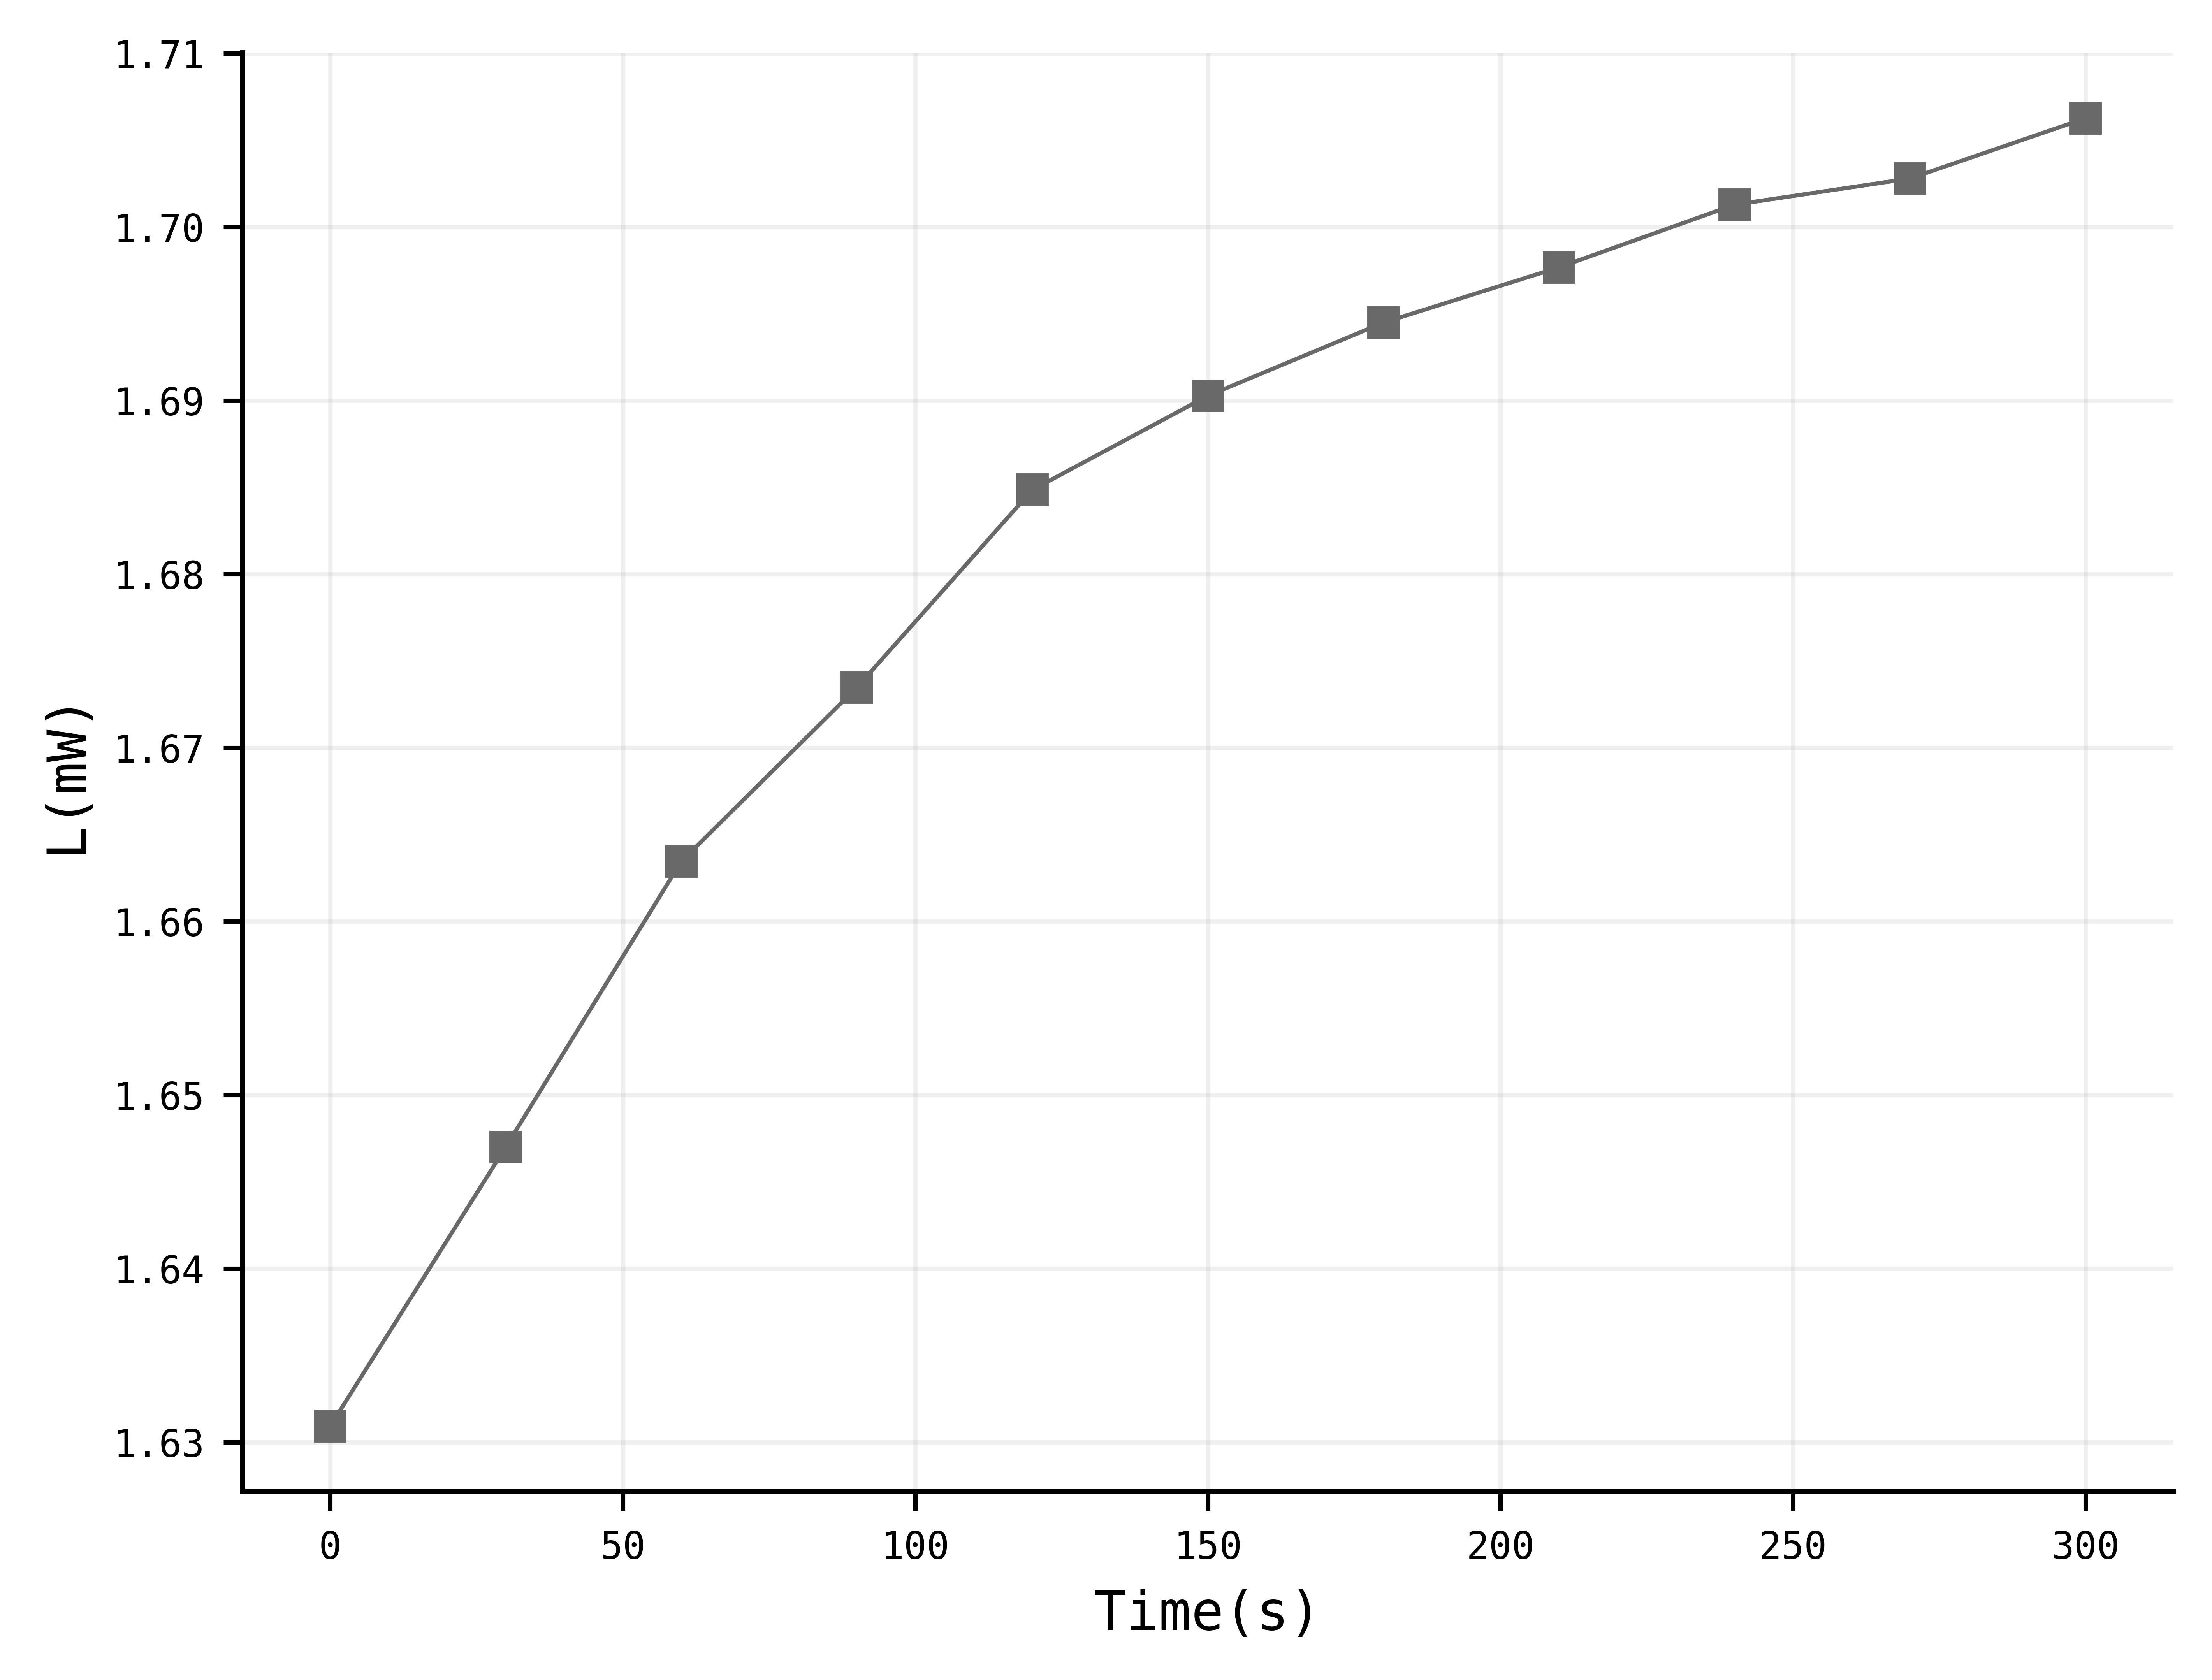
\includegraphics[width=0.475\columnwidth]{Quadrature_figure.png}}}%
    \quad
    \subfloat[\centering $V_{bias} \approx V_{max} \approx 8V$]{{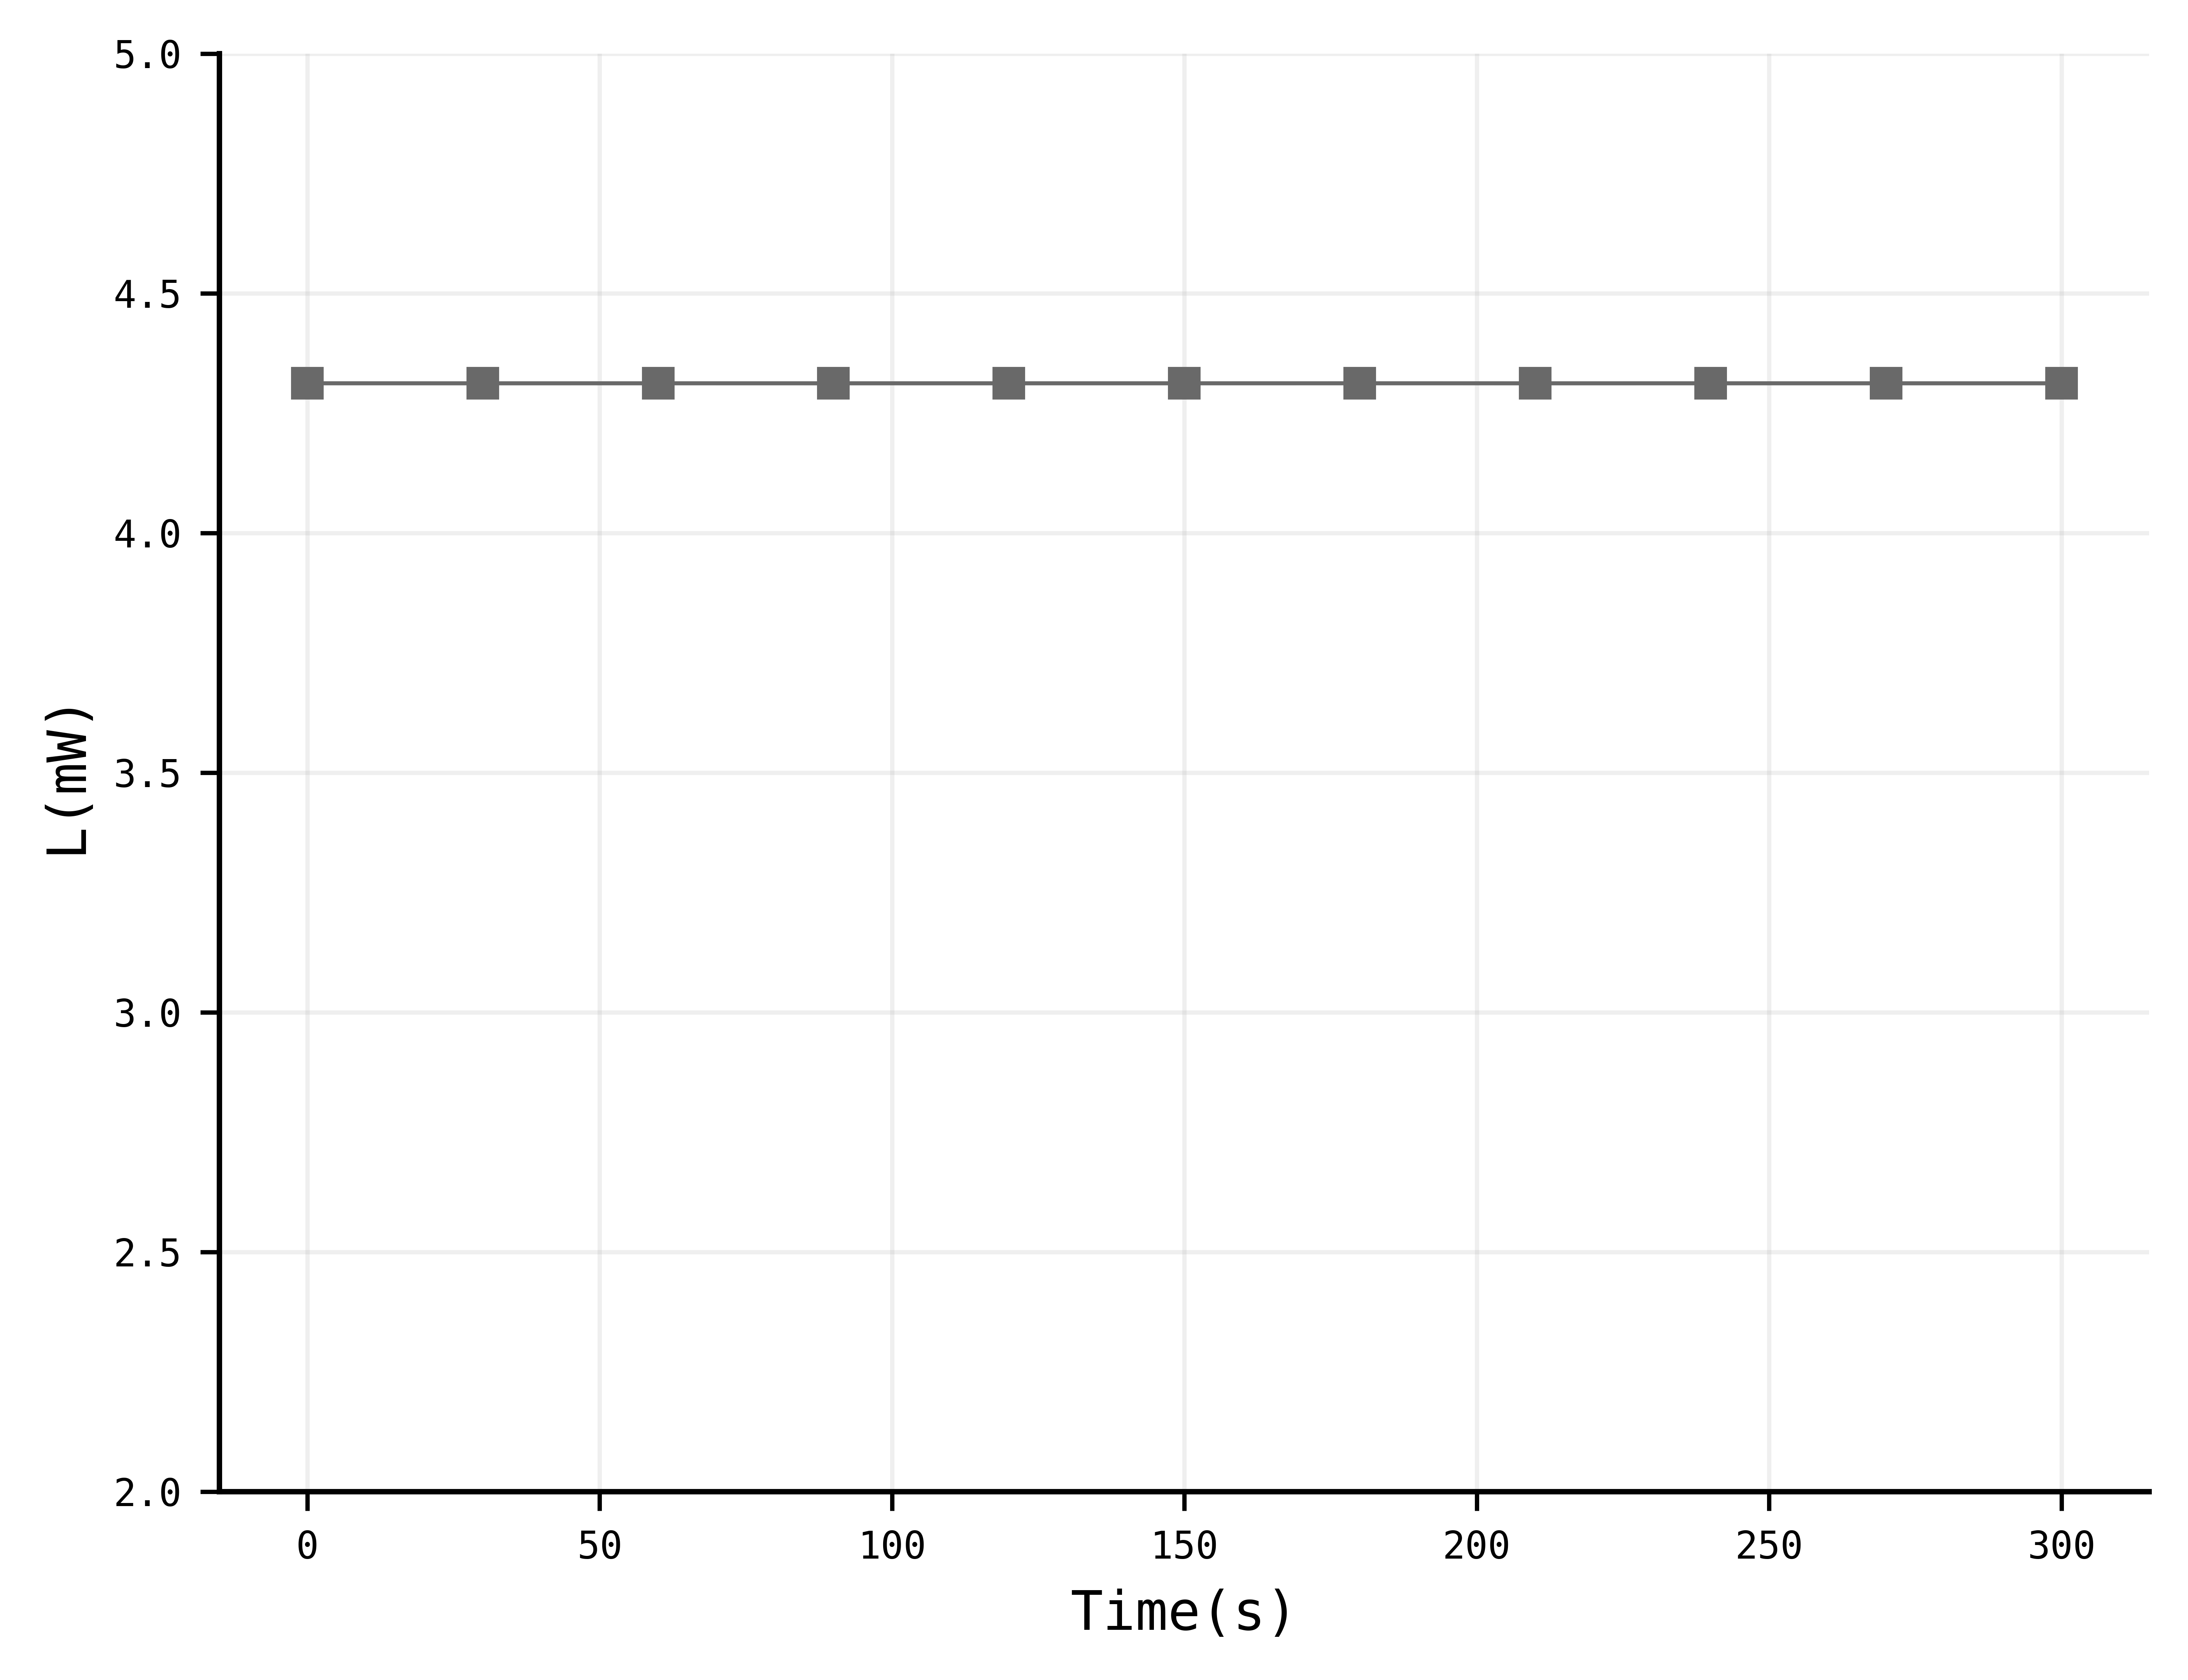
\includegraphics[width=0.475\columnwidth]{Maximum_figure.png}}}
    \caption{Further visualisation of transfer function drift at specific bias voltages. Sub-figures \textbf{(a)} and \textbf{(b)} show the power drift at the maximum and quadrature points of the transfer function. The drift is particularly obvious for the quadrature point and the maximum appears to be stable. This is to be expected, since the function drift is relatively slow (See Fig \ref{fig-transfer2}) it would take much longer to visualise.}
    \label{fig LI curves}%
    \vspace{-12pt}
    \label{fig-transfer3}
\end{figure}

\mychapter{3}{Experiment}
Throughout this section the RF clock source has been turned on and biased on the modulator via the amplifier at 12.5GHz (See Fig \ref{fig-setup}), unless otherwise stated. The purpose of this section is to analyse the impact of amplitude modulation applied to the modulator.
\section{Measurements/Data}\label{sec:data}
This section contains the OSA and Sampling Scope measurements for the output of the modulator at it's 3 critical points of relevance (minimum, maximum, quadrature). See Figures \ref{quad-m}, \ref{min-m}, \ref{max-m} and section \ref{sec:analysis} for a detailed discussion/analysis.
%Quadrature
\begin{figure}
    \centering
    \subfloat[\centering Sampling Scope]{{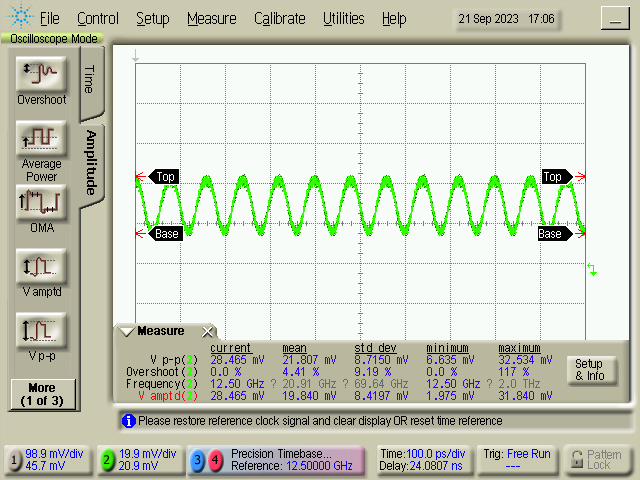
\includegraphics[width=0.475\columnwidth]{quad6v.png}}}
    \quad
    \subfloat[\centering OSA]{{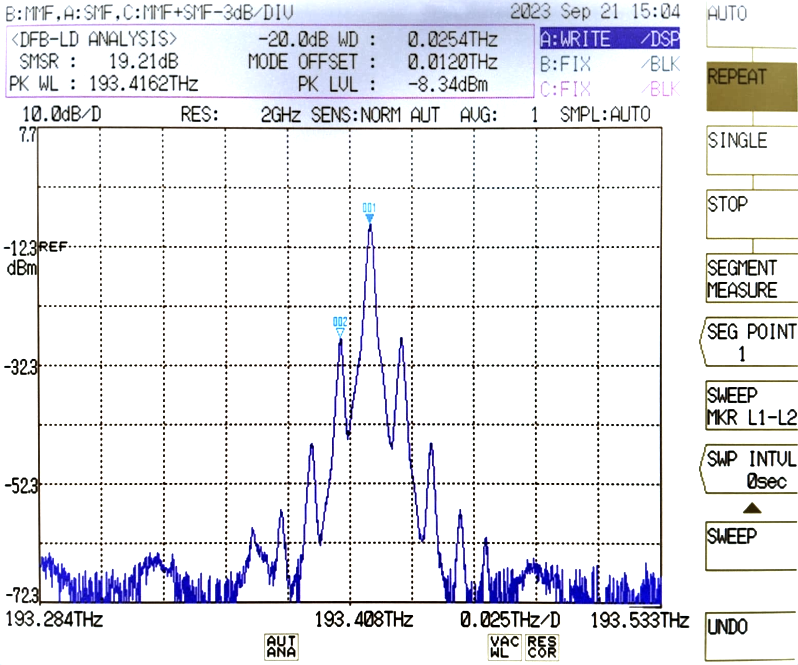
\includegraphics[width=0.475\columnwidth]{quadrature.png}}}\\
    \vspace{0.45cm}
    \text{$V_{bias}=5.8V \approx V_{\pi}$ | Mode offset: 0.012THz}
    \caption{Sampling Scope and OSA measurement for $V_{bias}=V_{\pi}$. The mode offset is 12.5GHz, indicated by light blue markers in \textbf{(b)}. \emph{Side bands} are now visible when modulating. The measured frequency is identical to the mode offset.}
    \label{quad-m}
    \vspace{-12pt}
\end{figure}
%Minimum
\begin{figure}
    \centering
    \subfloat[\centering Sampling Scope Measurement]{{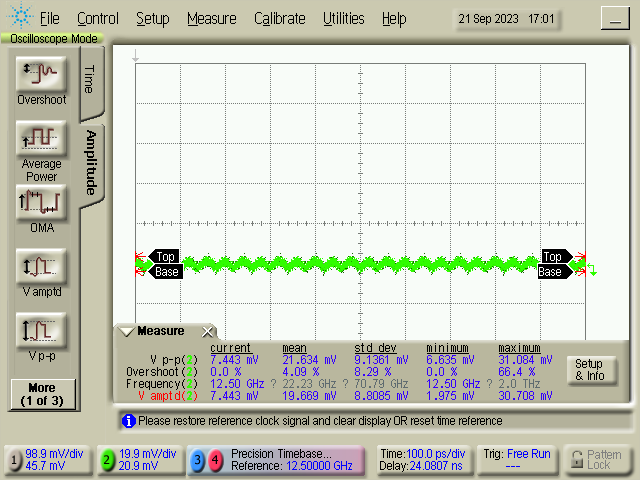
\includegraphics[width=0.475\columnwidth]{min4v.png}}}
    \quad
    \subfloat[\centering OSA Measurement]{{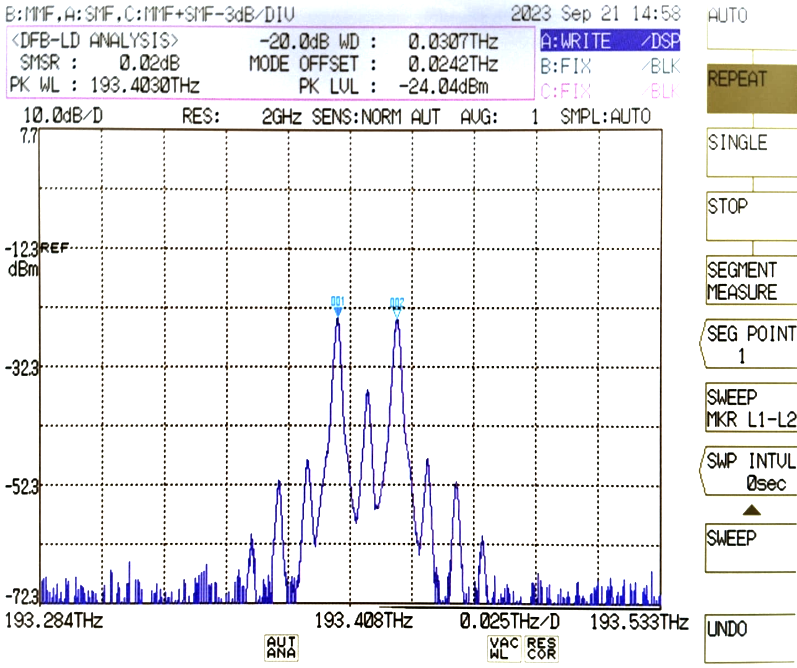
\includegraphics[width=0.475\columnwidth]{minimum.png}}}\\
    \vspace{0.45cm}
    \text{$V_{bias}=4V=V_{min}$ | Mode offset: 0.024THz}
    \caption{Sampling Scope and OSA measurement for $V_{bias}=4V=V_{min}$. This minimum point was found by observing the scope output in real-time. The previously determined $V_{min}$ was evidently not the minimum when observing the scope measurements - this was due to drift of the transfer function between measurements (overnight). The frequency observed in the scope measurement is \textbf{double} that of the quadrature measurement (See Fig \ref{quad-m}) and the mode offset is 24GHz, indicated by light blue markers in \textbf{(b)}. \textbf{The carrier signal intensity in the OSA and the average intensity in the scope have both decreased.}}
    \label{min-m}
    \vspace{-12pt}
\end{figure}
%Maximum
\begin{figure}
    \centering
    \subfloat[\centering Sampling Scope Measurement]{{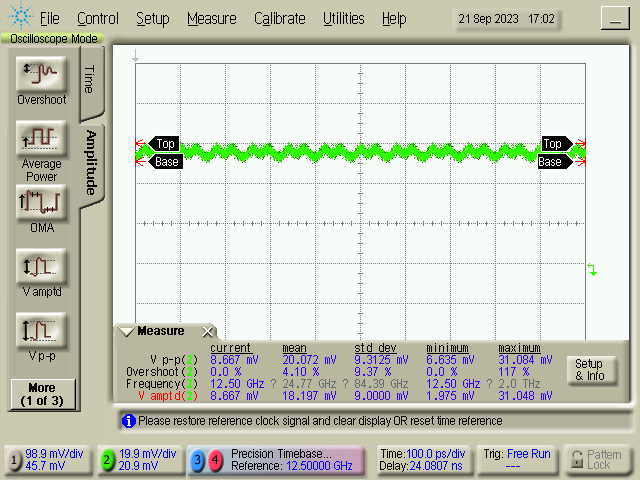
\includegraphics[width=0.475\columnwidth]{max8_6v.png}}}
    \quad
    \subfloat[\centering OSA Measurement]{{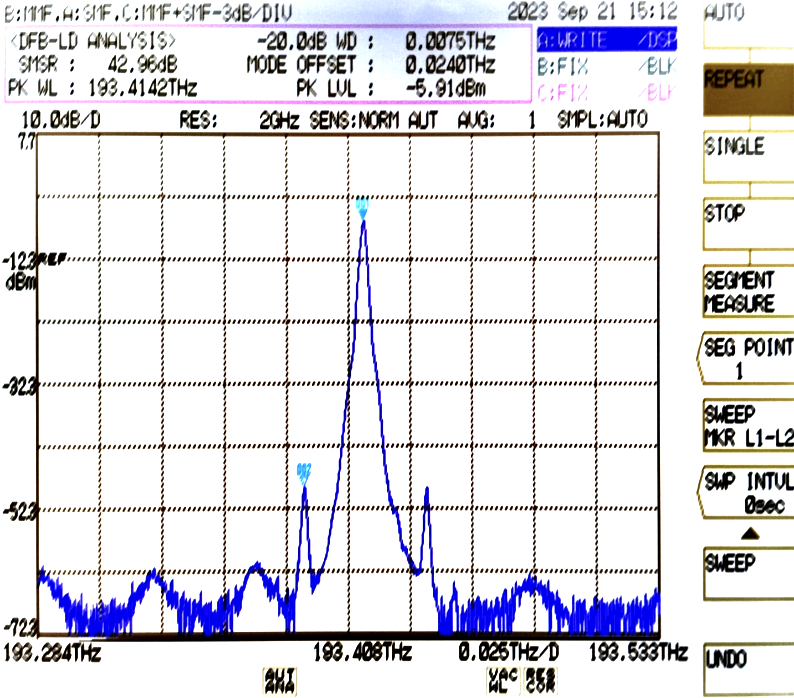
\includegraphics[width=0.475\columnwidth]{maximum.png}}}\\
    \vspace{0.45cm}
    \text{$V_{bias}=8.6V=V_{max}$ | Mode offset: 0.024THz}
    \caption{Sampling Scope and OSA measurement for $V_{bias}=8.6V=V_{max}$. This maximum point was found analogous to the method mentioned in Fig \ref{min-m}. The frequency observed in the scope measurement is \textbf{double} that of the quadrature measurement (See Fig \ref{quad-m}) and the mode offset is again 24GHz. \textbf{The carrier signal intensity in the OSA and the average intensity in the scope have both increased.}}
    \label{max-m}
    \vspace{-12pt}
\end{figure}

\section{Analysis and Discussion}\label{sec:analysis}
Fig \ref{comparison1} \textbf{(a)} shows a measurement without an applied oscillating bias (RF). It does not contain the various additional symmetric peaks evident in all other measurements. The peaks are spaced periodically at distances of 12.5GHz (RF clock) from the center. The center frequency in the modulated example \textbf{(b)} is generally referred to as the \emph{carrier frequency} in optical communication. The other peaks are referred to as \emph{side bands} and represent the modulation of the optical carrier signal - if the RF clock frequency were to change, so would the distance between peaks in the OSA measurement.

\begin{figure}
    \centering
    \subfloat[\centering No applied RF bias]{{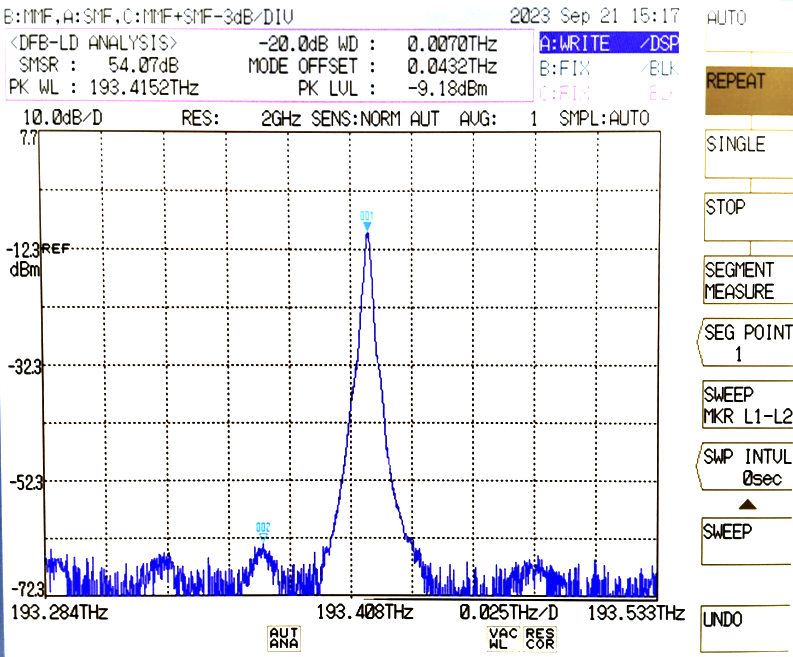
\includegraphics[width=0.475\columnwidth]{noRF.png}}}
    \quad
    \subfloat[\centering RF applied | $V_{bias}=V_{\pi}$]{{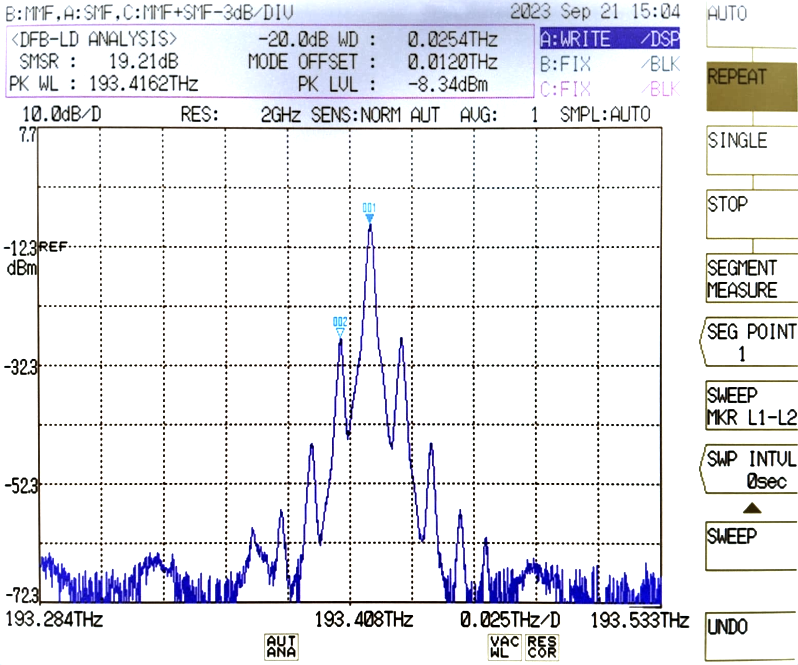
\includegraphics[width=0.475\columnwidth]{quadrature.png}}}\\
    \vspace{0.45cm}
    \caption{OSA measurements comparing the impact of amplitude modulation applied to the modulator and no modulation.}
    \label{comparison1}
    \vspace{-12pt}
\end{figure}

The transfer function measured in section \ref{sec:TF} tells us that measured intensities at bias voltages \textbf{symmetric} to a minimum/maximum on the transfer function will be equal. This is observed in the measurements shown in Figures \ref{quad-m}, \ref{min-m}, \ref{max-m}. They demonstrate that altering the bias voltage periodically (RF bias) causes light intensity oscillations at twice the frequency compared to the same operation at the quadrature point.

This phenomena also causes the variation in \emph{mode offsets} emphasised in Figures \ref{quad-m}, \ref{min-m}, \ref{max-m}. Similar to the frequency in the scope measurements, the mode offsets double for minimum/maximum points as the carrier signal increases/decreases analogous to the above. 

This can be linked to the average intensity of the sampled wave (scope measurements), which at minimum decreases with the reduction of the carrier signal intensity. The same trend occurs for the maximum, but with increased average intensity on the scope. 

Mode-offsets are identical to measured scope frequencies, demonstrated further in \ref{four}.

\subsection{Fourier Analysis}\label{four}
\begin{figure}
    \centering
    \subfloat[\centering ]{{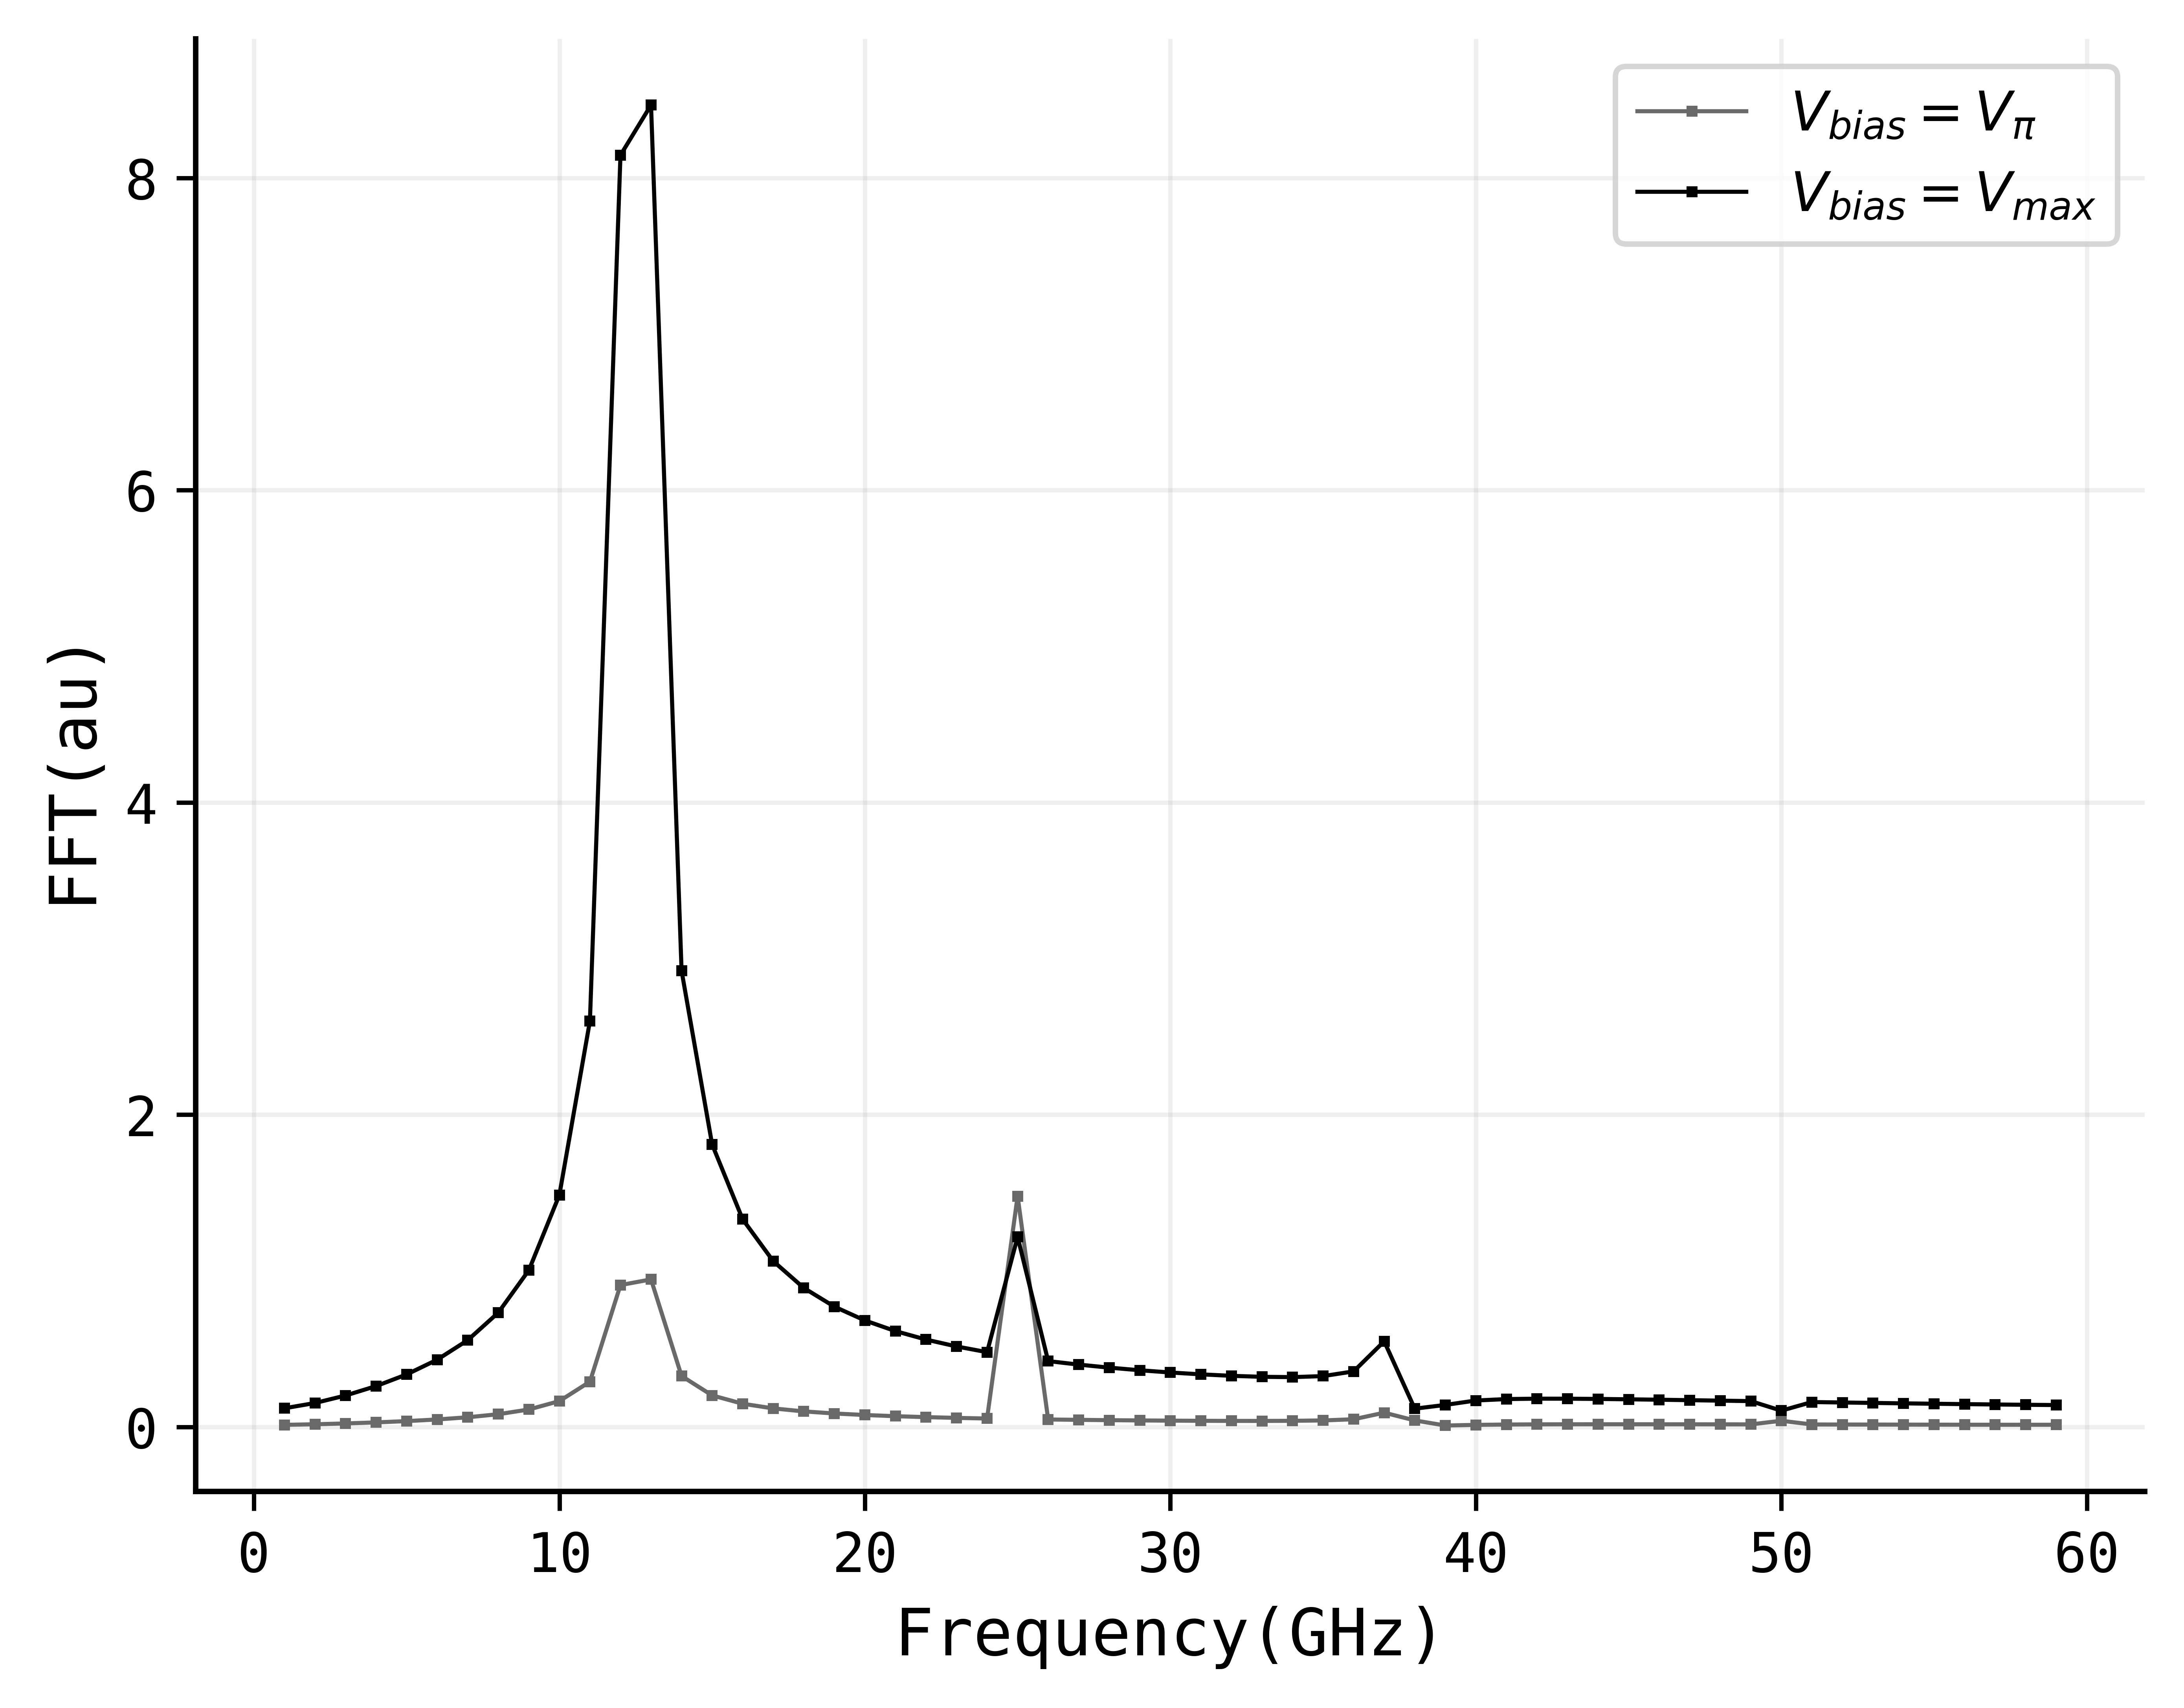
\includegraphics[width=0.475\columnwidth]{quadvsmax.png}}}
    \quad
    \subfloat[\centering ]{{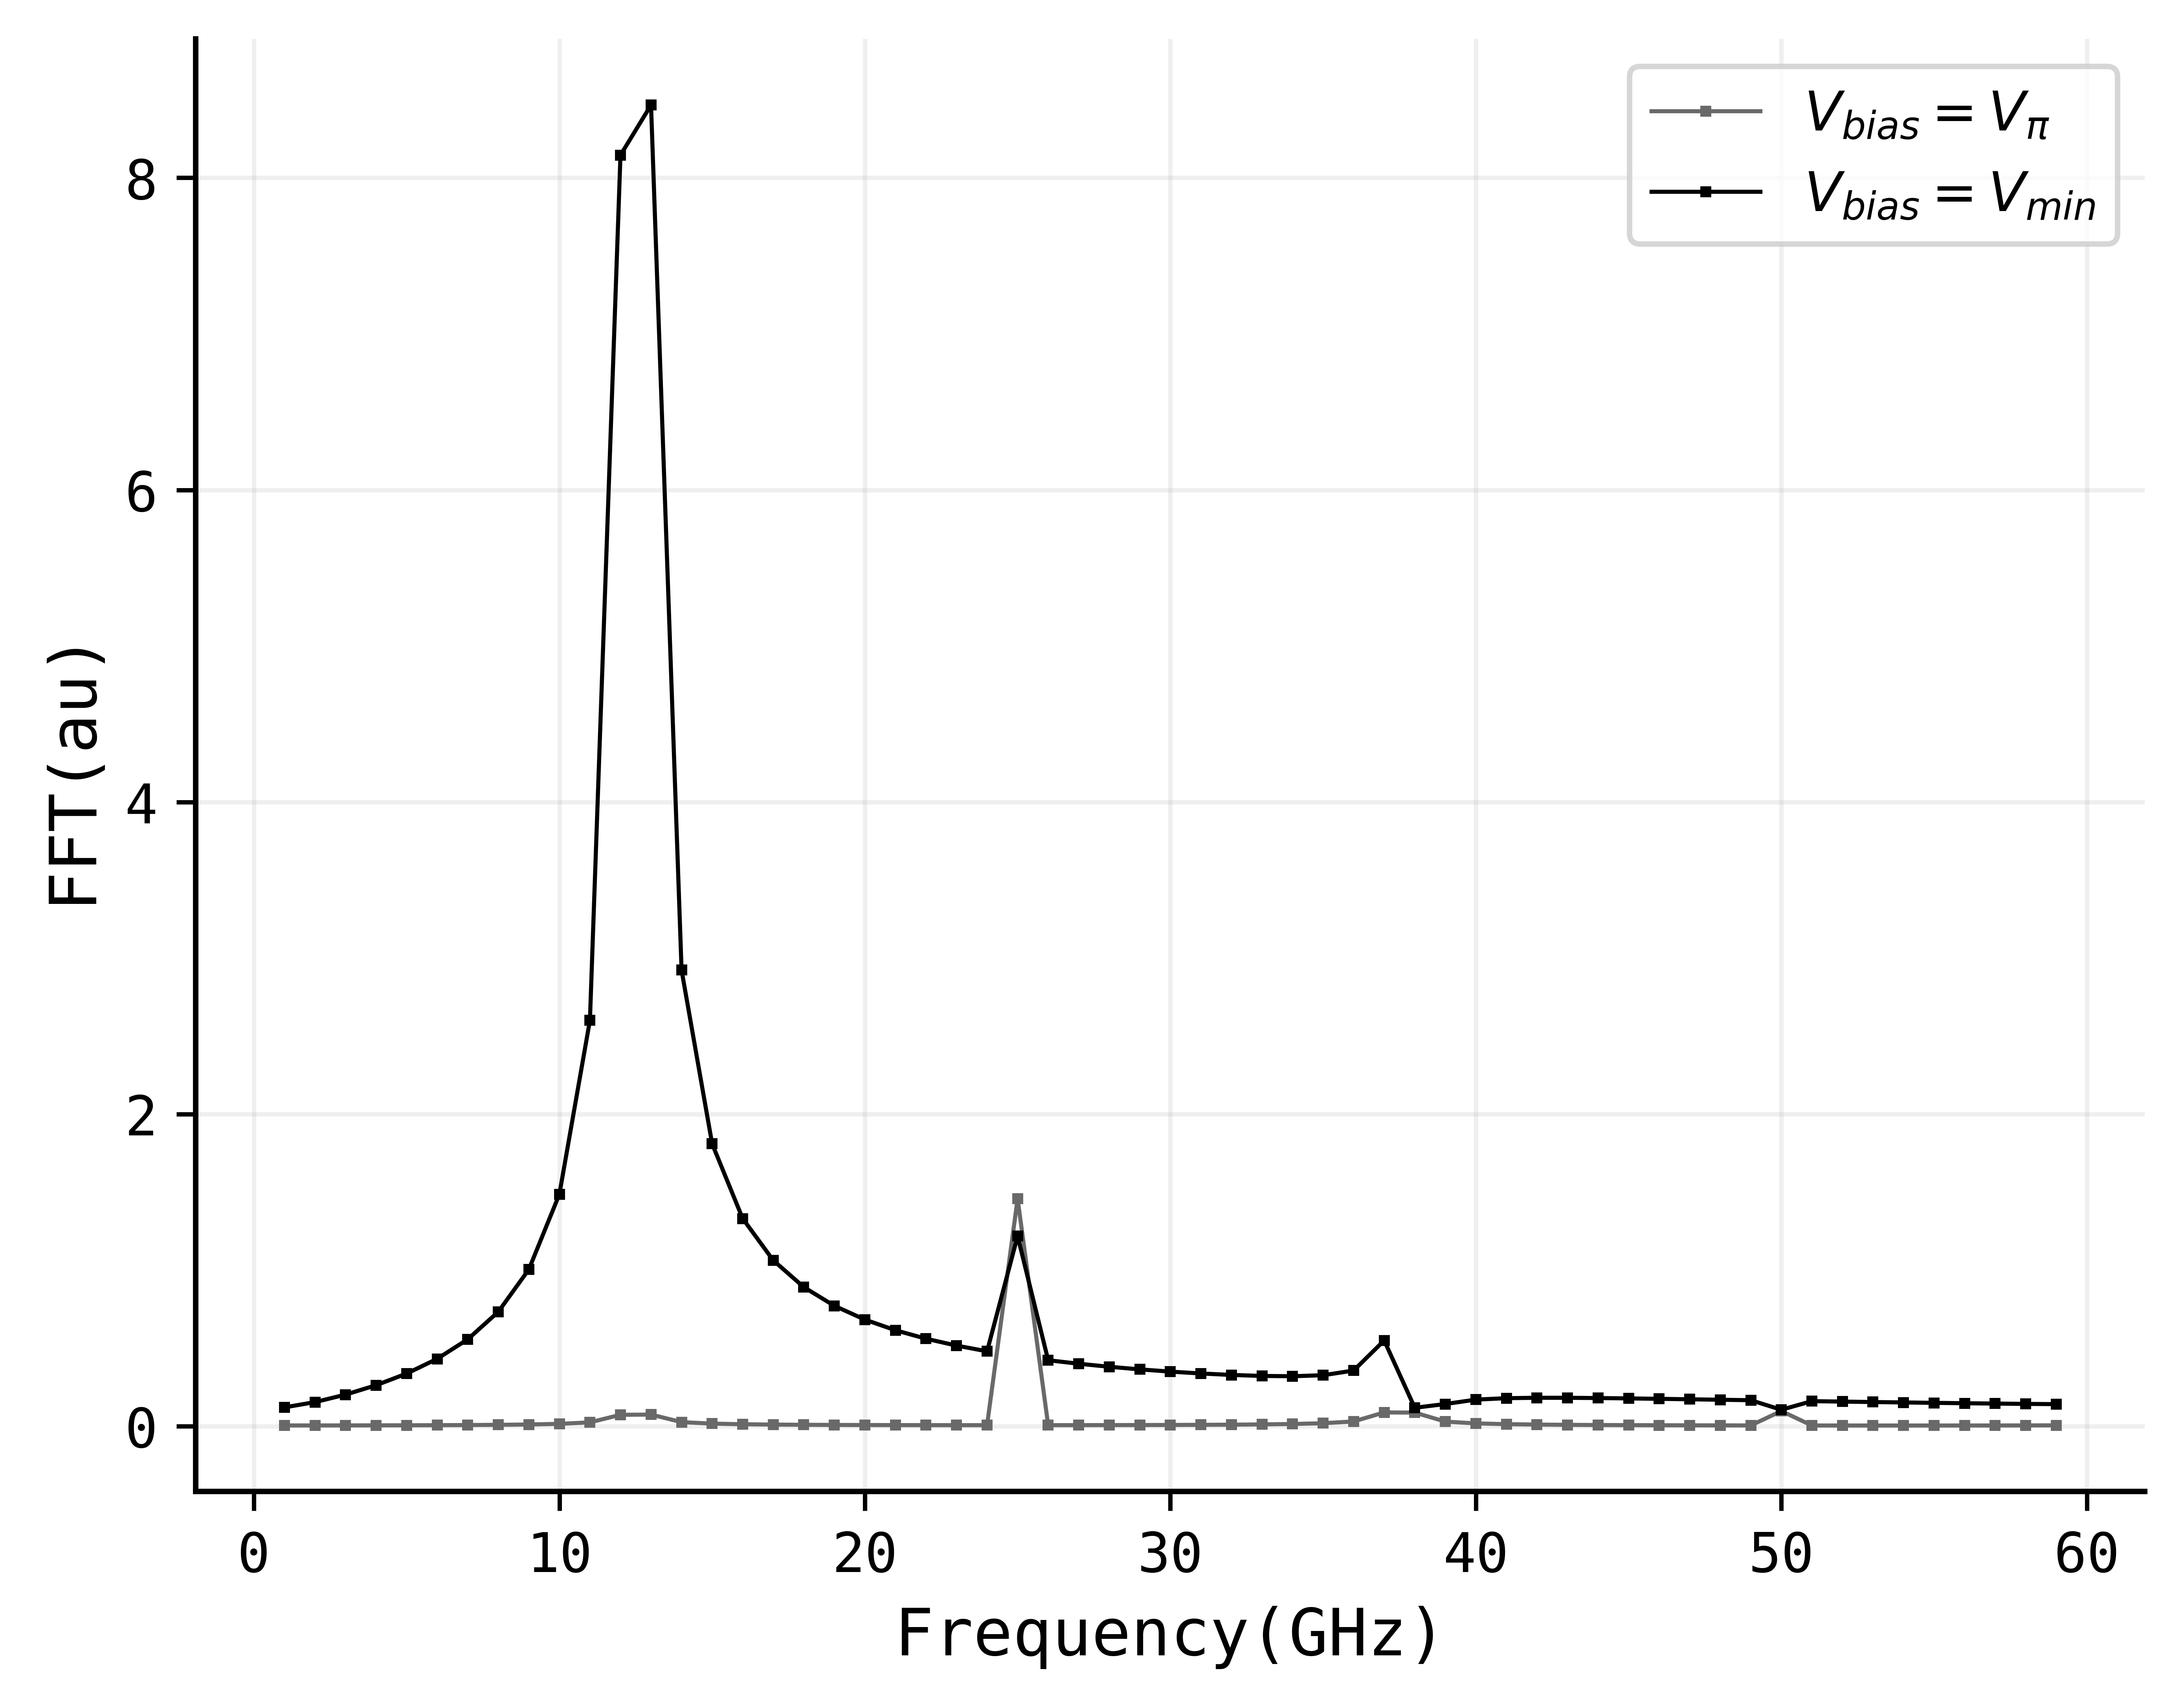
\includegraphics[width=0.475\columnwidth]{quadvsmin.png}}}
    \caption{Fast Fourier Transforms of raw data from sampling scope. \textbf{(a)} shows the FFT comparisons of the scope measurements at $V_{max}$ against $V_{\pi}$ and \textbf{(b)} shows a comparison of the $V_{min}$ against $V_{\pi}$. The related raw data is represented graphically in sub-figures \textbf{(a)} of \ref{quad-m}, \ref{min-m}, \ref{max-m}. There is peaks at the frequencies implied to be "mode offsets" in sections \ref{sec:data}, \ref{sec:analysis} in the transforms. The spectrum's have effectively been recreated without symmetry or a carrier signal.}
    \label{OSA-current}
    \vspace{-12pt}
\end{figure}
Fourier analysis (FFT's) of the raw scope data has recreated figures similar to the OSA measurements of section \ref{sec:data}. However, we see peaks at the frequencies implied to be "mode offsets" in sections \ref{sec:data}, \ref{sec:analysis}. For all measurements, the peaks of largest intensity directly corresponds to respective mode-offsets documented in section \ref{sec:data}. This makes some intuitive sense because we don't necessarily know what the wavelength of the laser is from just the scope measurements alone, all we can imply is the spectral components of the intensity signal.

\section{Further Measurements}
This section includes some further measurements and analysis completed out of interest and outside of the instructions of the brief.
\begin{figure}
    \centering
    \subfloat[\centering $V_{bias}\approx 1.5V$ ]{{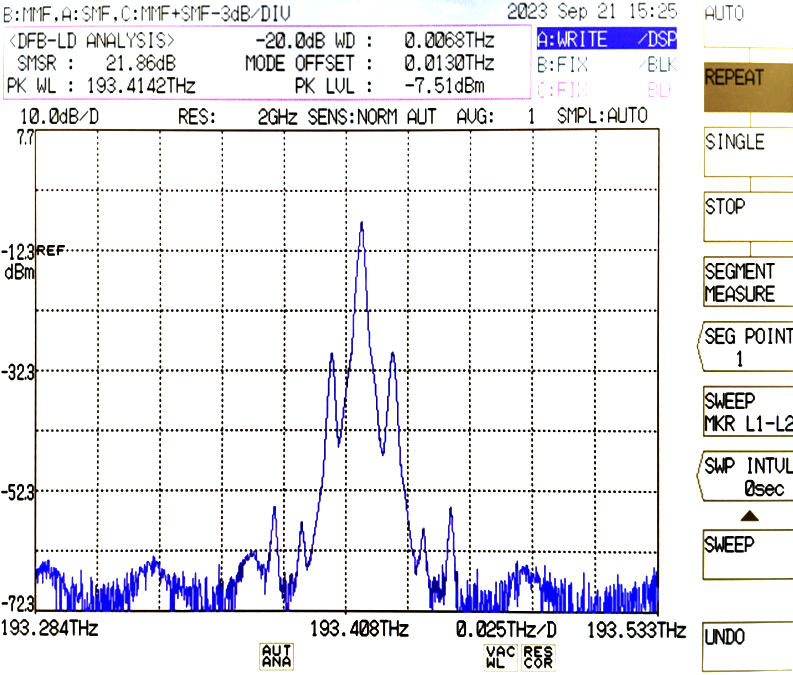
\includegraphics[width=0.475\columnwidth]{assymetric1V.png}}}
    \quad
    \subfloat[\centering $V_{bias}\approx 10.6V$]{{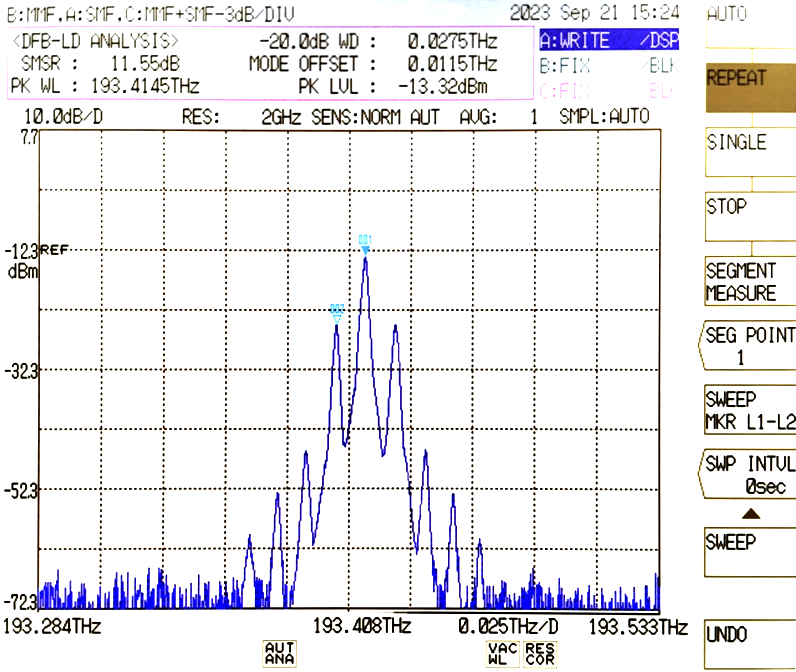
\includegraphics[width=0.475\columnwidth]{assymetric.png}}}
    \caption{Additional OSA measurements at \textbf{$V_{bias}\approx 1.5V$} and \textbf{$V_{bias}\approx 10.6V$} (10V was exceeded with permission). These are very interesting results because the behaviour is not what we should expect. These measurements were taken at what should have been quadrature points. \textbf{(b)} makes sense and is effectively identical to the quadrature measurements at $V_{bias}\approx 5.5V$, However \textbf{(a)} behave differently - the second side-bands have decreased to a minimum, which is not observed to be the case anywhere else on the transfer function. This is odd and unexpected behaviour, and may be related to some non-linear optical effects. See Fig \ref{extra2}.}
    \label{extra1}
    \vspace{-12pt}
    \label{extra}
\end{figure}
\subsection{Analysis/Observations}
\begin{figure}
    \centering
    \subfloat[\centering FFT]{{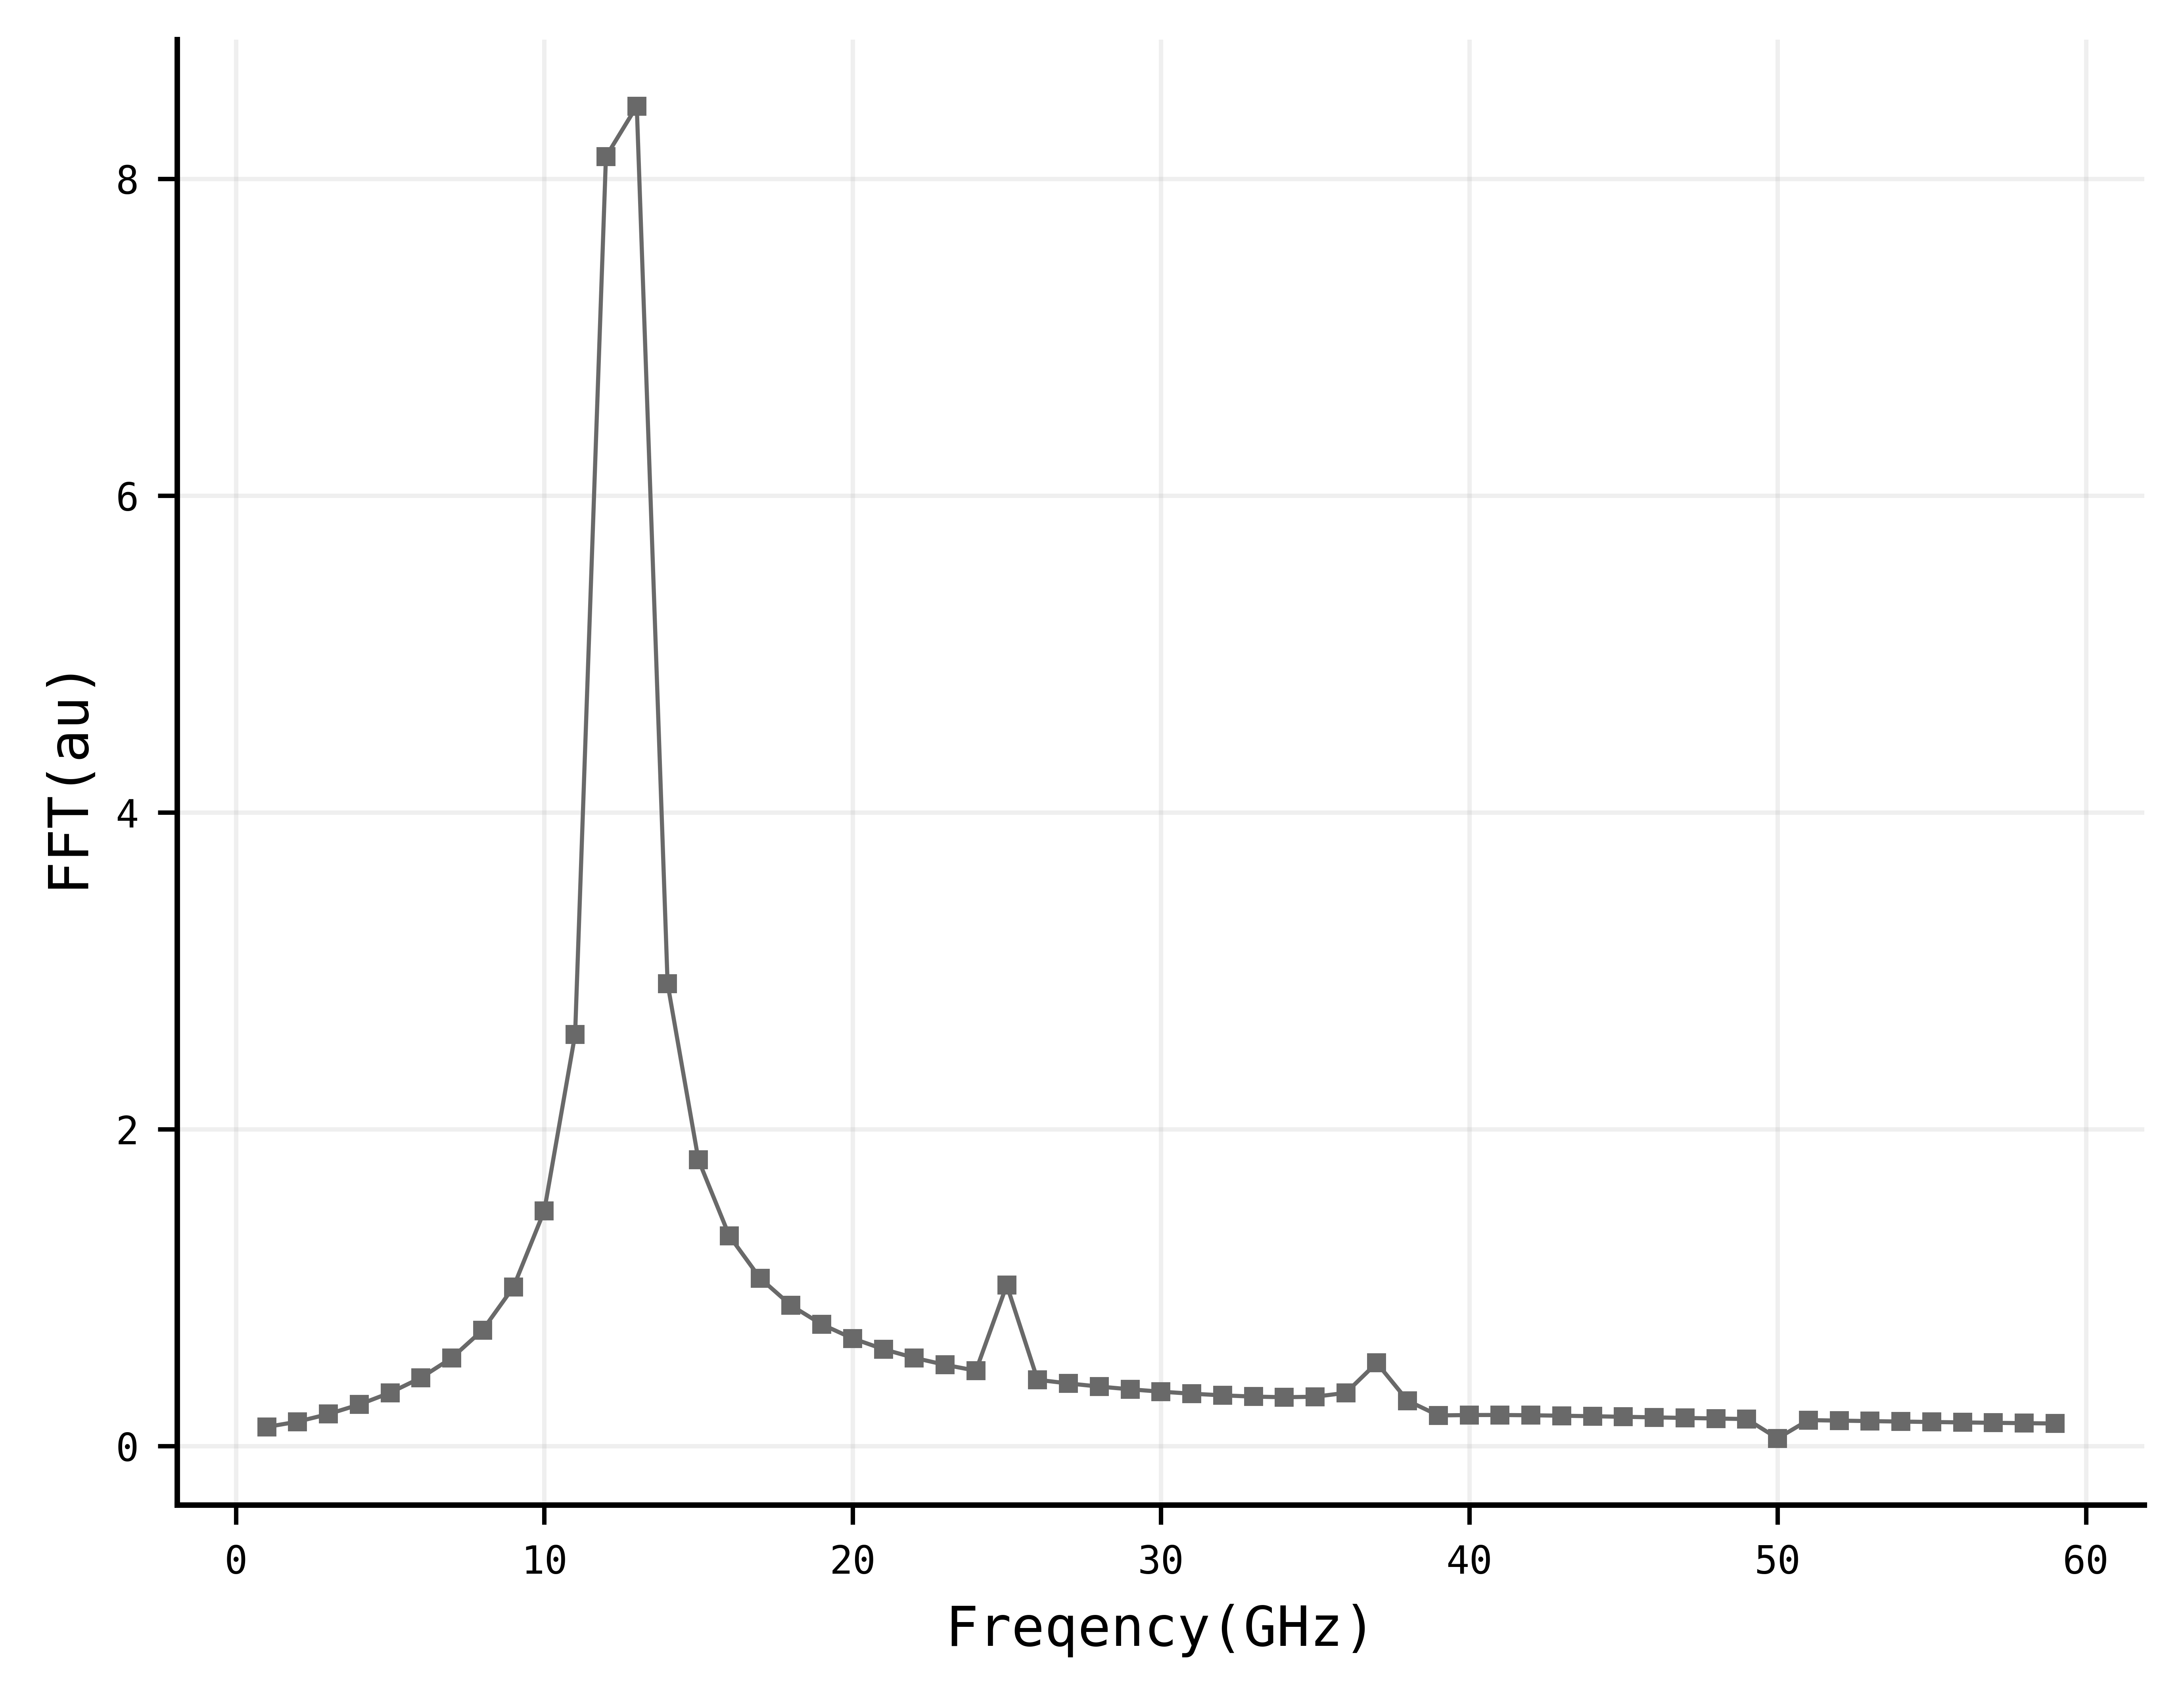
\includegraphics[width=0.475\columnwidth]{out1_2v (1)_figure.png}}}
    \quad
    \subfloat[\centering OSA]{{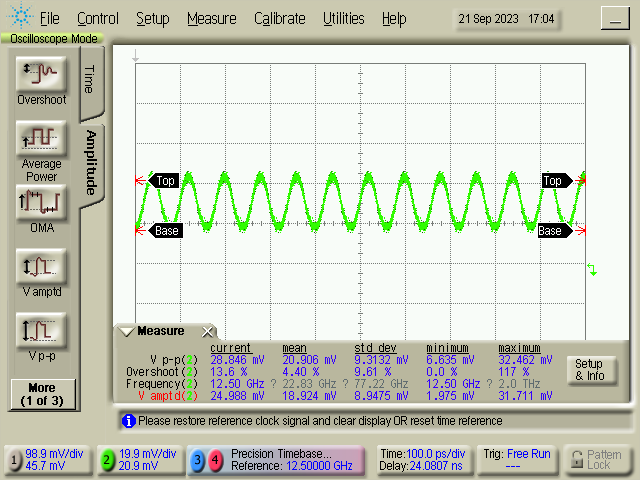
\includegraphics[width=0.475\columnwidth]{1_2v.png}}}
    \caption{Above \textbf{(a)} is an FFT of the raw data from Figure \ref{extra} \textbf{(a)}, and \textbf{(b)} is the graphed scope data - neither look dissimilar from what we would expect from the initial quadrature we concluded. What is rather surprising it that we get a more dominant peak at 24GHz than at 32GHz. It is difficult to conclude why this is - but it seems like the transforms consider mode off-sets independently of the carrier signal. }
    \label{extra2}
    \vspace{-12pt}
\end{figure}




\mychapter{4}{Conclusion}
The Mach Zehnder modoluator is a key instrument in optical communication world wide. A Mach Zehnder modulator modulates phase and subsequently the intensity of a light wave. Various instruments were characterised and discussed, notably a DFB laser which had some interesting temperature dependant effects, and the transfer function of the modulator, which drifted over time.

Section 3 analysed the impact of amplitude modulation applied to the modulator using an RF clock source and an amplifier. It was demonstrated that the position at which the voltage is oscillated on the transfer function (the DC bias voltage) has a significant effect on the optical spectrum and intensity variation of the modulators output. Raw sampling scope measurements were analysed for the critical points of relevance on the transfer function qualitatively and using Fourier transforms. Further measurements found that peaks in FT's related to 'mode-offsets' appeared to be independent of their distance from the carrier signal in OSA measurements.

This report hopefully serves as comprehensive study and demonstration of the underlying physics related to the Mach Zehnder modulator. 
\newpage
\vfill{}
\begin{thebibliography}{9}
\bibitem{freq} H. Taub, Donald L. Schilling, G. Saha \emph{Principles of Communication Systems}, 
\bibitem{lab_brief} University College Cork, School of Physics PY4113 Experiment 7 Lab Brief, \emph{Mach Zehnder Modulator, Tyndall National Institute} ISBN-13: 978-0074634540
\bibitem{ucclaser} University College Cork Laser Safety Guidelines and supplementary course notes (2022)
\bibitem{ucclaser-tables} University College Cork Laser Safety Tables (v5), \emph{"Annexes to course on; Lasers and Laser Safety"}
\bibitem{temp-dependance1} K. S. Mobarhan \emph{Test and Characterization of Laser Diodes:
Determination of Principal Parameters}, \textbf{Newport Corporation}
\bibitem{temp-dependance2} S. Vlasova, A. Vlasov, K. Alloyarov, T. Volkova \emph{Investigation of temperature dependence of
radiation from semiconductor lasers and light
emitting diodes}, \textbf{S Vlasova et al 2020 IOP Conf. Ser.: Earth Environ. Sci. 539 012137}
\bibitem{temp-dependance3} Zubkova S et al 2003 \emph{The temperature dependence of the band structure of polytypes 3C, 2H,
4H, and 6H silicon carbide}, \textbf{Fizika i tehnika poluprovodnikov 37 257}
\bibitem{temp-dependance4} Vainshtein I et al 1999 \emph{The applicability of the empirical Varshni relation for the temperature
dependence of the band gap}, \textbf{Fizika tverdogo tela 41 994}
\bibitem{laser1} Zeller Wolfgang, Nähle Lars, Fuchs, Peter Gerschuetz, Florian  Hildebrandt Lars, Koeth Johannes. (2010). \emph{DFB Lasers Between 760 nm and 16 um for Sensing Applications. Sensors (Basel, Switzerland). 10. 2492-510. 10.3390/s100402492.}
\bibitem{modulator-spec} PowerBit SD-40 40 Gb/s Intensity Modulator Data Sheet
\bibitem{PER} R. F. Stevens \emph{POLARISATION EXTINCTION RATIO – MEASUREMENT
REQUIREMENTS FOR OPTICAL COMMUNICATION SYSTEMS}, \textbf{NPL REPORT CETM 41, National Physical Laboratory, Teddington, Middlesex}
\bibitem{energy} Appl. Phys. 103, 093110 (2008) \emph{Measurement of the junction temperature in high power light-emitting diodes from the high energy wing of the electro-luminescence band}
\end{thebibliography}
\newpage
\appendix
\chapter{Formulas}
\textbf{Table \ref{OSA-t}:}
\begin{equation}
    \lambda_T = 1545.05nm+[px(1550.05nm)-px(1545.05nm)]\times\left[\frac{5nm}{px(1550.05nm)-px(PEAK)}\right]
    \label{A.1}
\end{equation}

\chapter{Source Code}\label{code}
This code would have been used to extract the junction temperature of the DFB laser. Shown is an example of the functioning code with image and text output using example measurements from a microLED.

    \begin{tcolorbox}[breakable, size=fbox, boxrule=1pt, pad at break*=1mm,colback=cellbackground, colframe=cellborder]
\prompt{In}{incolor}{5}{\boxspacing}
\begin{Verbatim}[commandchars=\\\{\}]
\PY{c+c1}{\PYZsh{} \PYZhy{}*\PYZhy{} coding: utf\PYZhy{}8 \PYZhy{}*\PYZhy{}}
\PY{l+s+sd}{\PYZdq{}\PYZdq{}\PYZdq{}}
\PY{l+s+sd}{Created on Fri Jul 14 11:24:53 2023}
\PY{l+s+sd}{@author: jordan.walsh}

\PY{l+s+sd}{\PYZdq{}\PYZdq{}\PYZdq{}}

\PY{k+kn}{from} \PY{n+nn}{glob} \PY{k+kn}{import} \PY{n}{glob}
\PY{k+kn}{import} \PY{n+nn}{numpy} \PY{k}{as} \PY{n+nn}{np}
\PY{k+kn}{import} \PY{n+nn}{matplotlib}\PY{n+nn}{.}\PY{n+nn}{pyplot} \PY{k}{as} \PY{n+nn}{plt} 
\PY{k+kn}{import} \PY{n+nn}{os}
\PY{k+kn}{from} \PY{n+nn}{pylab} \PY{k+kn}{import} \PY{o}{*}
\PY{k+kn}{import} \PY{n+nn}{sys}

\PY{n}{index} \PY{o}{=} \PY{l+m+mi}{0}
\PY{n}{peaks} \PY{o}{=} \PY{p}{[}\PY{p}{]}
\PY{n}{data} \PY{o}{=} \PY{p}{[}\PY{p}{]}
\PY{n}{h} \PY{o}{=} \PY{l+m+mf}{6.62607015e\PYZhy{}34} \PY{c+c1}{\PYZsh{}planck}
\PY{n}{c} \PY{o}{=} \PY{l+m+mf}{2.99792458e8} \PY{c+c1}{\PYZsh{}speed of light}
\PY{n}{e} \PY{o}{=} \PY{l+m+mf}{1.60217663e\PYZhy{}19} \PY{c+c1}{\PYZsh{}electron}
\PY{n}{k} \PY{o}{=} \PY{l+m+mf}{1.380649e\PYZhy{}23} \PY{c+c1}{\PYZsh{}boltzmann}
\PY{n}{J\PYZus{}eV} \PY{o}{=} \PY{l+m+mi}{1}\PY{o}{/}\PY{p}{(}\PY{l+m+mf}{6.242e18}\PY{p}{)} \PY{c+c1}{\PYZsh{}Joules / eV}
\PY{n}{i} \PY{o}{=} \PY{l+m+mi}{0}

\PY{c+c1}{\PYZsh{}\PYZhy{}\PYZhy{}\PYZhy{}\PYZhy{}\PYZhy{}\PYZhy{}\PYZhy{}\PYZhy{}\PYZhy{}\PYZhy{}\PYZhy{}\PYZhy{}\PYZhy{}\PYZhy{}\PYZhy{}\PYZhy{}\PYZhy{}\PYZhy{}\PYZhy{}\PYZhy{}\PYZhy{}\PYZhy{}\PYZhy{}\PYZhy{}\PYZhy{}\PYZhy{}\PYZhy{}\PYZhy{}\PYZhy{}\PYZhy{}\PYZhy{} PLOT CONTROLS \PYZhy{}\PYZhy{}\PYZhy{}\PYZhy{}\PYZhy{}\PYZhy{}\PYZhy{}\PYZhy{}\PYZhy{}\PYZhy{}\PYZhy{}\PYZhy{}\PYZhy{}\PYZhy{}\PYZhy{}\PYZhy{}\PYZhy{}\PYZhy{}\PYZhy{}\PYZhy{}\PYZhy{}\PYZhy{}\PYZhy{}\PYZhy{}\PYZhy{}\PYZhy{}\PYZhy{}\PYZhy{}\PYZhy{}\PYZhy{}\PYZhy{}\PYZsh{}}

\PY{n}{path} \PY{o}{=}\PY{l+s+sa}{r}\PY{l+s+s2}{\PYZdq{}}\PY{l+s+s2}{Z:}\PY{l+s+s2}{\PYZbs{}}\PY{l+s+s2}{Tyndall}\PY{l+s+s2}{\PYZbs{}}\PY{l+s+s2}{LED measurements 210723 (MS)}\PY{l+s+s2}{\PYZbs{}}\PY{l+s+s2}{green}\PY{l+s+s2}{\PYZdq{}}
\PY{n}{PLOT\PYZus{}LIMIT} \PY{o}{=} \PY{p}{[}\PY{l+m+mi}{450}\PY{p}{,} \PY{l+m+mi}{600}\PY{p}{]} \PY{c+c1}{\PYZsh{} wavelength limits in nm}
\PY{n}{Y\PYZus{}LIMIT} \PY{o}{=} \PY{p}{[}\PY{l+m+mf}{1e\PYZhy{}3}\PY{p}{,} \PY{l+m+mi}{2}\PY{p}{]} \PY{c+c1}{\PYZsh{} enforced only for log plots [lower, upper] \PYZhy{} leave blank for auto}

\PY{n}{INCLUDE\PYZus{}ENERGY\PYZus{}SCALE} \PY{o}{=} \PY{k+kc}{True} \PY{c+c1}{\PYZsh{} Wavelegnth \PYZam{} energy plot \PYZhy{} energy is indication only, intensity not accounted for}
\PY{n}{PLOT\PYZus{}INDIVIDUAL\PYZus{}SPECTRUMS} \PY{o}{=} \PY{k+kc}{False} \PY{c+c1}{\PYZsh{} Plot all files individually}
\PY{n}{CREATE\PYZus{}COMPILED\PYZus{}PLOT} \PY{o}{=} \PY{k+kc}{True} \PY{c+c1}{\PYZsh{} Plot all spectrums in one}

\PY{n}{ENERGY\PYZus{}ONLY} \PY{o}{=} \PY{k+kc}{True} \PY{c+c1}{\PYZsh{} Energy (eV) only mode || overrides INCLUDE\PYZus{}ENERGY\PYZus{}SCALE if enabled and rescales to reflect true intensity of energy}
\PY{n}{ALL\PYZus{}PLOTS\PYZus{}MAX\PYZus{}1} \PY{o}{=} \PY{k+kc}{False} \PY{c+c1}{\PYZsh{} Plots with all spectrums will be normalised to have the same maximum (1)}

\PY{n}{LOG\PYZus{}PLOT\PYZus{}FITTING} \PY{o}{=} \PY{k+kc}{True} \PY{c+c1}{\PYZsh{} [Carrier Temp] Return information for boltzmann stats from specified FIT\PYZus{}RANGE [Least Squares fit]}
\PY{n}{FIT\PYZus{}RANGE} \PY{o}{=} \PY{p}{[}\PY{l+m+mi}{480}\PY{p}{,} \PY{l+m+mi}{500}\PY{p}{]} \PY{c+c1}{\PYZsh{} wavelength in nm || These options allow you to find carrier temperature for ENERGY\PYZus{}ONLY plots}

\PY{c+c1}{\PYZsh{}\PYZhy{}\PYZhy{}\PYZhy{}\PYZhy{}\PYZhy{}\PYZhy{}\PYZhy{}\PYZhy{}\PYZhy{}\PYZhy{}\PYZhy{}\PYZhy{}\PYZhy{}\PYZhy{}\PYZhy{}\PYZhy{}\PYZhy{}\PYZhy{}\PYZhy{}\PYZhy{}\PYZhy{}\PYZhy{}\PYZhy{}\PYZhy{}\PYZhy{}\PYZhy{}\PYZhy{}\PYZhy{}\PYZhy{}\PYZhy{}\PYZhy{}\PYZhy{}\PYZhy{}\PYZhy{}\PYZhy{}\PYZhy{}\PYZhy{}\PYZhy{}\PYZhy{}\PYZhy{}\PYZhy{}\PYZhy{}\PYZhy{}\PYZhy{}\PYZhy{}\PYZhy{}\PYZhy{}\PYZhy{}\PYZhy{}\PYZhy{}\PYZhy{}\PYZhy{}\PYZhy{}\PYZhy{}\PYZhy{}\PYZhy{}\PYZhy{}\PYZhy{}\PYZhy{}\PYZhy{}\PYZhy{}\PYZhy{}\PYZhy{}\PYZhy{}\PYZhy{}\PYZhy{}\PYZhy{}\PYZhy{}\PYZhy{}\PYZhy{}\PYZhy{}\PYZhy{}\PYZhy{}\PYZhy{}\PYZhy{}\PYZhy{}\PYZhy{}\PYZsh{}}

\PY{c+c1}{\PYZsh{} WARNING: TICKS ON BOTTOM AND TOP MUST BE ALLIGNED FOR ENERGY SCALE TO BE DISPLAYED CORRECTLY}

\PY{c+c1}{\PYZsh{}\PYZhy{}\PYZhy{}\PYZhy{}\PYZhy{}\PYZhy{}\PYZhy{}\PYZhy{}\PYZhy{}\PYZhy{}\PYZhy{}\PYZhy{}\PYZhy{}\PYZhy{}\PYZhy{}\PYZhy{}\PYZhy{}\PYZhy{}\PYZhy{}\PYZhy{}\PYZhy{}\PYZhy{}\PYZhy{}\PYZhy{}\PYZhy{}\PYZhy{}\PYZhy{}\PYZhy{}\PYZhy{}\PYZhy{}\PYZhy{}\PYZhy{}\PYZhy{}\PYZhy{}\PYZhy{}\PYZhy{}\PYZhy{}\PYZhy{}\PYZhy{}\PYZhy{}\PYZhy{}\PYZhy{}\PYZhy{}\PYZhy{}\PYZhy{}\PYZhy{}\PYZhy{}\PYZhy{}\PYZhy{}\PYZhy{}\PYZhy{}\PYZhy{}\PYZhy{}\PYZhy{}\PYZhy{}\PYZhy{}\PYZhy{}\PYZhy{}\PYZhy{}\PYZhy{}\PYZhy{}\PYZhy{}\PYZhy{}\PYZhy{}\PYZhy{}\PYZhy{}\PYZhy{}\PYZhy{}\PYZhy{}\PYZhy{}\PYZhy{}\PYZhy{}\PYZhy{}\PYZhy{}\PYZhy{}\PYZhy{}\PYZhy{}\PYZhy{}\PYZsh{}}

\PY{k}{def} \PY{n+nf}{preventDivisionByZero}\PY{p}{(}\PY{n}{some\PYZus{}array}\PY{p}{)}\PY{p}{:}
    \PY{n}{corrected\PYZus{}array} \PY{o}{=} \PY{n}{some\PYZus{}array}\PY{o}{.}\PY{n}{copy}\PY{p}{(}\PY{p}{)}
    \PY{k}{for} \PY{n}{i}\PY{p}{,} \PY{n}{entry} \PY{o+ow}{in} \PY{n+nb}{enumerate}\PY{p}{(}\PY{n}{some\PYZus{}array}\PY{p}{)}\PY{p}{:}
        \PY{c+c1}{\PYZsh{} If element is zero, set to some small value}
        \PY{k}{if} \PY{n+nb}{abs}\PY{p}{(}\PY{n}{entry}\PY{p}{)} \PY{o}{\PYZlt{}} \PY{n}{sys}\PY{o}{.}\PY{n}{float\PYZus{}info}\PY{o}{.}\PY{n}{epsilon}\PY{p}{:}
            \PY{n}{corrected\PYZus{}array}\PY{p}{[}\PY{n}{i}\PY{p}{]} \PY{o}{=} \PY{n}{sys}\PY{o}{.}\PY{n}{float\PYZus{}info}\PY{o}{.}\PY{n}{epsilon}
    \PY{k}{return} \PY{n}{corrected\PYZus{}array}

\PY{c+c1}{\PYZsh{} Converting wavelength (nm) to energy (eV)}
\PY{k}{def} \PY{n+nf}{WLtoE}\PY{p}{(}\PY{n}{wl}\PY{p}{,} \PY{n}{label}\PY{p}{)}\PY{p}{:}
    \PY{k}{if} \PY{n+nb}{str}\PY{p}{(}\PY{n+nb}{type}\PY{p}{(}\PY{n}{wl}\PY{p}{)}\PY{p}{)} \PY{o}{==} \PY{l+s+s2}{\PYZdq{}}\PY{l+s+s2}{\PYZlt{}class }\PY{l+s+s2}{\PYZsq{}}\PY{l+s+s2}{list}\PY{l+s+s2}{\PYZsq{}}\PY{l+s+s2}{\PYZgt{}}\PY{l+s+s2}{\PYZdq{}}\PY{p}{:} \PY{c+c1}{\PYZsh{}check for single value or list of values}
        \PY{c+c1}{\PYZsh{} Prevent division by zero error}
        \PY{k}{for} \PY{n}{i} \PY{o+ow}{in} \PY{n+nb}{range}\PY{p}{(}\PY{n+nb}{len}\PY{p}{(}\PY{n}{wl}\PY{p}{)}\PY{p}{)}\PY{p}{:}
            \PY{n}{wl}\PY{p}{[}\PY{n}{i}\PY{p}{]} \PY{o}{=} \PY{n+nb}{float}\PY{p}{(}\PY{n}{wl}\PY{p}{[}\PY{n}{i}\PY{p}{]}\PY{p}{)}
        \PY{n}{wl} \PY{o}{=} \PY{n}{preventDivisionByZero}\PY{p}{(}\PY{n}{wl}\PY{p}{)}
        \PY{n}{wl} \PY{o}{=} \PY{n}{np}\PY{o}{.}\PY{n}{array}\PY{p}{(}\PY{n}{wl}\PY{p}{)}
        
    \PY{n}{E\PYZus{}eV} \PY{o}{=} \PY{l+m+mi}{1243} \PY{o}{/} \PY{n}{wl} \PY{c+c1}{\PYZsh{}h*c=1243}
    \PY{k}{if} \PY{n}{label} \PY{o}{==} \PY{l+s+s1}{\PYZsq{}}\PY{l+s+s1}{label}\PY{l+s+s1}{\PYZsq{}}\PY{p}{:} \PY{c+c1}{\PYZsh{}what is the purpose of conversion (i.e for scale labels or important data)}
        \PY{k}{for} \PY{n}{i} \PY{o+ow}{in} \PY{n+nb}{range}\PY{p}{(}\PY{n+nb}{len}\PY{p}{(}\PY{n}{E\PYZus{}eV}\PY{p}{)}\PY{p}{)}\PY{p}{:}
            \PY{n}{E\PYZus{}eV}\PY{p}{[}\PY{n}{i}\PY{p}{]} \PY{o}{=} \PY{n+nb}{float}\PY{p}{(}\PY{l+s+s2}{\PYZdq{}}\PY{l+s+si}{\PYZob{}:.2f\PYZcb{}}\PY{l+s+s2}{\PYZdq{}}\PY{o}{.}\PY{n}{format}\PY{p}{(}\PY{n}{E\PYZus{}eV}\PY{p}{[}\PY{n}{i}\PY{p}{]}\PY{p}{)}\PY{p}{)}
    \PY{k}{return} \PY{n}{E\PYZus{}eV}

\PY{k}{def} \PY{n+nf}{add\PYZus{}energy\PYZus{}scale}\PY{p}{(}\PY{n}{plt}\PY{p}{)}\PY{p}{:} \PY{c+c1}{\PYZsh{}converts photon wavelength to energy, adds scale on top \PYZhy{} does not account for reltive intensity change}
    \PY{n}{ax} \PY{o}{=} \PY{n}{plt}\PY{o}{.}\PY{n}{gca}\PY{p}{(}\PY{p}{)}
    \PY{n}{labels} \PY{o}{=} \PY{n}{ax}\PY{o}{.}\PY{n}{get\PYZus{}xticks}\PY{p}{(}\PY{p}{)}
    \PY{n}{ax2} \PY{o}{=} \PY{n}{ax}\PY{o}{.}\PY{n}{twiny}\PY{p}{(}\PY{p}{)}
    \PY{n}{ax2}\PY{o}{.}\PY{n}{set\PYZus{}xlim}\PY{p}{(}\PY{n}{PLOT\PYZus{}LIMIT}\PY{p}{)}
    \PY{n}{ax2}\PY{o}{.}\PY{n}{set\PYZus{}xticks}\PY{p}{(}\PY{n}{labels}\PY{p}{,} \PY{n}{WLtoE}\PY{p}{(}\PY{n}{labels}\PY{p}{,} \PY{l+s+s1}{\PYZsq{}}\PY{l+s+s1}{label}\PY{l+s+s1}{\PYZsq{}}\PY{p}{)}\PY{p}{)} \PY{c+c1}{\PYZsh{}locations, corresponding labels}
    \PY{n}{ax2}\PY{o}{.}\PY{n}{set\PYZus{}xlabel}\PY{p}{(}\PY{l+s+s1}{\PYZsq{}}\PY{l+s+s1}{Energy (eV)}\PY{l+s+s1}{\PYZsq{}}\PY{p}{,} \PY{n}{fontsize}\PY{o}{=}\PY{l+m+mi}{8}\PY{p}{)}

\PY{k}{def} \PY{n+nf}{convert\PYZus{}wl\PYZus{}intensity\PYZus{}to\PYZus{}energy\PYZus{}intensity}\PY{p}{(}\PY{n}{y}\PY{p}{,} \PY{n}{x}\PY{p}{)}\PY{p}{:} \PY{c+c1}{\PYZsh{}x must be wl in nm}
    \PY{n}{i} \PY{o}{=} \PY{l+m+mi}{0}
    \PY{k}{try}\PY{p}{:} \PY{c+c1}{\PYZsh{}if fails its because index is out of range (y isnt an array/list)}
        \PY{n}{y} \PY{o}{=} \PY{n}{np}\PY{o}{.}\PY{n}{array}\PY{p}{(}\PY{n}{y}\PY{p}{)}
        \PY{n}{x} \PY{o}{=} \PY{n}{np}\PY{o}{.}\PY{n}{array}\PY{p}{(}\PY{n}{x}\PY{p}{)}
        \PY{k}{for} \PY{n}{i} \PY{o+ow}{in} \PY{n+nb}{range}\PY{p}{(}\PY{n+nb}{len}\PY{p}{(}\PY{n}{y}\PY{p}{)}\PY{p}{)}\PY{p}{:}
            \PY{n}{y}\PY{p}{[}\PY{n}{i}\PY{p}{]} \PY{o}{=} \PY{n}{y}\PY{p}{[}\PY{n}{i}\PY{p}{]} \PY{o}{*} \PY{p}{(}\PY{n}{x}\PY{p}{[}\PY{n}{i}\PY{p}{]}\PY{o}{*}\PY{l+m+mf}{1e\PYZhy{}9}\PY{p}{)}\PY{o}{\PYZca{}}\PY{l+m+mi}{2} \PY{o}{/} \PY{p}{(}\PY{n}{h}\PY{o}{*}\PY{n}{c}\PY{p}{)}
    \PY{k}{except} \PY{n+ne}{Exception} \PY{k}{as} \PY{n}{err}\PY{p}{:} \PY{c+c1}{\PYZsh{}I am aware that this is the most lazy way possible to do this}
        \PY{c+c1}{\PYZsh{}print(\PYZdq{}conversion not array [\PYZob{}\PYZcb{}]\PYZdq{}.format(err))}
        \PY{n}{y} \PY{o}{=} \PY{n}{y} \PY{o}{*} \PY{p}{(}\PY{n}{x}\PY{o}{*}\PY{l+m+mf}{1e\PYZhy{}9}\PY{p}{)}\PY{o}{*}\PY{o}{*}\PY{l+m+mi}{2} \PY{o}{/} \PY{p}{(}\PY{n}{h}\PY{o}{*}\PY{n}{c}\PY{p}{)}
    \PY{k}{return} \PY{n}{y}

\PY{k}{def} \PY{n+nf}{plot\PYZus{}graph}\PY{p}{(}\PY{n}{x}\PY{p}{,} \PY{n}{y}\PY{p}{,} \PY{n}{top\PYZus{}energy\PYZus{}scale}\PY{p}{,} \PY{n}{energy\PYZus{}scale\PYZus{}only}\PY{p}{)}\PY{p}{:} \PY{c+c1}{\PYZsh{}create a single plot}
    \PY{n}{labels} \PY{o}{=} \PY{p}{[}\PY{p}{]}
    \PY{n}{plt}\PY{o}{.}\PY{n}{figure}\PY{p}{(}\PY{p}{)}
    \PY{k}{if} \PY{n}{energy\PYZus{}scale\PYZus{}only} \PY{o}{==} \PY{k+kc}{True}\PY{p}{:}
        \PY{n}{y} \PY{o}{=} \PY{n}{convert\PYZus{}wl\PYZus{}intensity\PYZus{}to\PYZus{}energy\PYZus{}intensity}\PY{p}{(}\PY{n}{y}\PY{p}{,} \PY{n}{x}\PY{p}{)}
        \PY{n}{x} \PY{o}{=} \PY{n}{WLtoE}\PY{p}{(}\PY{n}{x}\PY{p}{,} \PY{l+s+s1}{\PYZsq{}}\PY{l+s+s1}{data}\PY{l+s+s1}{\PYZsq{}}\PY{p}{)}
        \PY{n}{plt}\PY{o}{.}\PY{n}{xlim}\PY{p}{(}\PY{n}{WLtoE}\PY{p}{(}\PY{n}{PLOT\PYZus{}LIMIT}\PY{p}{,} \PY{l+s+s1}{\PYZsq{}}\PY{l+s+s1}{data}\PY{l+s+s1}{\PYZsq{}}\PY{p}{)}\PY{p}{)}
    \PY{k}{else}\PY{p}{:}
        \PY{n}{plt}\PY{o}{.}\PY{n}{xlim}\PY{p}{(}\PY{n}{PLOT\PYZus{}LIMIT}\PY{p}{)}
    \PY{n}{plt}\PY{o}{.}\PY{n}{plot}\PY{p}{(}\PY{n}{x}\PY{p}{,} \PY{n}{y}\PY{p}{,} \PY{n}{linewidth} \PY{o}{=} \PY{l+m+mi}{1}\PY{p}{,} \PY{n}{color} \PY{o}{=} \PY{l+s+s1}{\PYZsq{}}\PY{l+s+s1}{\PYZsh{}0c00b4ff}\PY{l+s+s1}{\PYZsq{}}\PY{p}{)}
    \PY{n}{plt}\PY{o}{.}\PY{n}{title}\PY{p}{(}\PY{l+s+sa}{f}\PY{l+s+s2}{\PYZdq{}}\PY{l+s+s2}{\PYZdq{}}\PY{p}{)}
    \PY{n}{plt}\PY{o}{.}\PY{n}{xlabel}\PY{p}{(}\PY{l+s+s2}{\PYZdq{}}\PY{l+s+s2}{Wavelength (nm)}\PY{l+s+s2}{\PYZdq{}}\PY{p}{,} \PY{n}{fontsize}\PY{o}{=}\PY{l+m+mi}{8}\PY{p}{)}
    \PY{n}{plt}\PY{o}{.}\PY{n}{ylabel}\PY{p}{(}\PY{l+s+s2}{\PYZdq{}}\PY{l+s+s2}{Intensity (au)}\PY{l+s+s2}{\PYZdq{}}\PY{p}{,}  \PY{n}{fontsize}\PY{o}{=}\PY{l+m+mi}{8}\PY{p}{)}
    \PY{n}{plt}\PY{o}{.}\PY{n}{xticks}\PY{p}{(}\PY{n}{fontsize} \PY{o}{=} \PY{l+m+mi}{7}\PY{p}{)}
    \PY{n}{plt}\PY{o}{.}\PY{n}{yticks}\PY{p}{(}\PY{n}{fontsize} \PY{o}{=} \PY{l+m+mi}{7}\PY{p}{)}
    
    \PY{n}{matplotlib}\PY{o}{.}\PY{n}{pyplot}\PY{o}{.}\PY{n}{figtext}\PY{p}{(}\PY{l+m+mf}{0.6}\PY{p}{,}\PY{l+m+mf}{0.8}\PY{p}{,} \PY{l+s+sa}{f}\PY{l+s+s2}{\PYZdq{}}\PY{l+s+s2}{Max = }\PY{l+s+si}{\PYZob{}}\PY{n}{maximum}\PY{l+s+si}{\PYZcb{}}\PY{l+s+s2}{nm}\PY{l+s+s2}{\PYZdq{}}\PY{p}{,} \PY{n}{fontsize} \PY{o}{=} \PY{l+s+s2}{\PYZdq{}}\PY{l+s+s2}{medium}\PY{l+s+s2}{\PYZdq{}}\PY{p}{)}
    \PY{n}{plt}\PY{o}{.}\PY{n}{grid}\PY{p}{(}\PY{k+kc}{True}\PY{p}{,} \PY{n}{alpha}\PY{o}{=}\PY{l+m+mf}{0.5}\PY{p}{)}
    \PY{n}{labels} \PY{o}{=} \PY{n}{np}\PY{o}{.}\PY{n}{array}\PY{p}{(}\PY{n}{labels}\PY{p}{)}
    \PY{k}{if} \PY{n}{top\PYZus{}energy\PYZus{}scale} \PY{o}{==} \PY{k+kc}{True} \PY{o+ow}{and} \PY{n}{energy\PYZus{}scale\PYZus{}only} \PY{o}{==} \PY{k+kc}{False}\PY{p}{:}
        \PY{n}{add\PYZus{}energy\PYZus{}scale}\PY{p}{(}\PY{n}{plt}\PY{p}{)}
    \PY{n}{plt}\PY{o}{.}\PY{n}{savefig}\PY{p}{(}\PY{l+s+sa}{f}\PY{l+s+s1}{\PYZsq{}}\PY{l+s+si}{\PYZob{}}\PY{n}{file}\PY{l+s+si}{\PYZcb{}}\PY{l+s+s1}{\PYZus{}figure.png}\PY{l+s+s1}{\PYZsq{}}\PY{p}{,} \PY{n}{dpi} \PY{o}{=} \PY{l+m+mi}{1000}\PY{p}{,} \PY{n}{bbox\PYZus{}inches}\PY{o}{=}\PY{l+s+s1}{\PYZsq{}}\PY{l+s+s1}{tight}\PY{l+s+s1}{\PYZsq{}}\PY{p}{)}
    \PY{n}{plt}\PY{o}{.}\PY{n}{show}\PY{p}{(}\PY{p}{)}
    
\PY{k}{def} \PY{n+nf}{return\PYZus{}boltzmann}\PY{p}{(}\PY{n}{x}\PY{p}{,} \PY{n}{y}\PY{p}{)}\PY{p}{:} \PY{c+c1}{\PYZsh{}extract exponential features between bounds elected}
    \PY{n}{x} \PY{o}{=} \PY{n}{np}\PY{o}{.}\PY{n}{array}\PY{p}{(}\PY{n}{x}\PY{p}{)}
    \PY{n}{y} \PY{o}{=} \PY{n}{np}\PY{o}{.}\PY{n}{array}\PY{p}{(}\PY{n}{y}\PY{p}{)}
    
    \PY{k}{try}\PY{p}{:}
        \PY{k}{if} \PY{n}{ENERGY\PYZus{}ONLY} \PY{o}{==} \PY{k+kc}{True}\PY{p}{:}
            \PY{n}{E\PYZus{}FIT} \PY{o}{=} \PY{n}{WLtoE}\PY{p}{(}\PY{n}{FIT\PYZus{}RANGE}\PY{p}{,} \PY{l+s+s1}{\PYZsq{}}\PY{l+s+s1}{data}\PY{l+s+s1}{\PYZsq{}}\PY{p}{)}
            \PY{n}{indices} \PY{o}{=} \PY{n}{np}\PY{o}{.}\PY{n}{where}\PY{p}{(}\PY{p}{(}\PY{n}{x} \PY{o}{\PYZgt{}}\PY{o}{=} \PY{n+nb}{min}\PY{p}{(}\PY{n}{E\PYZus{}FIT}\PY{p}{)}\PY{p}{)} \PY{o}{\PYZam{}} \PY{p}{(}\PY{n}{x} \PY{o}{\PYZlt{}}\PY{o}{=} \PY{n+nb}{max}\PY{p}{(}\PY{n}{E\PYZus{}FIT}\PY{p}{)}\PY{p}{)}\PY{p}{)}
        \PY{k}{else}\PY{p}{:}
            \PY{n}{indices} \PY{o}{=} \PY{n}{np}\PY{o}{.}\PY{n}{where}\PY{p}{(}\PY{p}{(}\PY{n}{x} \PY{o}{\PYZgt{}}\PY{o}{=} \PY{n+nb}{min}\PY{p}{(}\PY{n}{FIT\PYZus{}RANGE}\PY{p}{)}\PY{p}{)} \PY{o}{\PYZam{}} \PY{p}{(}\PY{n}{x} \PY{o}{\PYZlt{}}\PY{o}{=} \PY{n+nb}{max}\PY{p}{(}\PY{n}{FIT\PYZus{}RANGE}\PY{p}{)}\PY{p}{)}\PY{p}{)} \PY{c+c1}{\PYZsh{}extrapolate range for fitting}
        \PY{k}{if} \PY{n}{indices}\PY{p}{[}\PY{l+m+mi}{0}\PY{p}{]}\PY{o}{.}\PY{n}{size} \PY{o}{\PYZlt{}} \PY{l+m+mi}{1}\PY{p}{:}
            \PY{k}{raise} \PY{n+ne}{Exception}\PY{p}{(}\PY{l+s+s2}{\PYZdq{}}\PY{l+s+s2}{Failed to find indices in range provided}\PY{l+s+s2}{\PYZdq{}}\PY{p}{)}
    \PY{k}{except} \PY{n+ne}{Exception} \PY{k}{as} \PY{n}{err}\PY{p}{:}
        \PY{n+nb}{print}\PY{p}{(}\PY{l+s+s2}{\PYZdq{}}\PY{l+s+s2}{ERROR [}\PY{l+s+si}{\PYZob{}\PYZcb{}}\PY{l+s+s2}{]}\PY{l+s+s2}{\PYZdq{}}\PY{o}{.}\PY{n}{format}\PY{p}{(}\PY{n}{err}\PY{p}{)}\PY{p}{)}
    
    \PY{n}{x\PYZus{}fit} \PY{o}{=} \PY{n}{x}\PY{p}{[}\PY{n}{indices}\PY{p}{]}
    \PY{n}{y\PYZus{}fit} \PY{o}{=} \PY{n}{np}\PY{o}{.}\PY{n}{log}\PY{p}{(}\PY{n}{y}\PY{p}{[}\PY{n}{indices}\PY{p}{]}\PY{p}{)}
    \PY{n}{deg} \PY{o}{=} \PY{l+m+mi}{1}    
    \PY{n}{p}\PY{p}{,} \PY{n}{cov} \PY{o}{=} \PY{n}{np}\PY{o}{.}\PY{n}{polyfit}\PY{p}{(}\PY{n}{x\PYZus{}fit}\PY{p}{,} \PY{n}{y\PYZus{}fit}\PY{p}{,} \PY{n}{deg}\PY{p}{,} \PY{n}{full}\PY{o}{=}\PY{k+kc}{False}\PY{p}{,} \PY{n}{cov}\PY{o}{=}\PY{k+kc}{True}\PY{p}{)}    
    \PY{n}{a} \PY{o}{=} \PY{n}{np}\PY{o}{.}\PY{n}{exp}\PY{p}{(}\PY{n}{p}\PY{p}{[}\PY{n}{deg}\PY{p}{]}\PY{p}{)}  
    \PY{n}{b} \PY{o}{=} \PY{n}{p}\PY{p}{[}\PY{l+m+mi}{0}\PY{p}{]}
    \PY{n}{poly\PYZus{}error} \PY{o}{=} \PY{n}{sqrt}\PY{p}{(}\PY{n}{diag}\PY{p}{(}\PY{n}{cov}\PY{p}{)}\PY{p}{[}\PY{l+m+mi}{1}\PY{p}{]}\PY{p}{)}
    \PY{n+nb}{print}\PY{p}{(}\PY{n}{p}\PY{p}{)}
    \PY{n+nb}{print}\PY{p}{(}\PY{n}{cov}\PY{p}{)}
    \PY{n+nb}{print}\PY{p}{(}\PY{n}{poly\PYZus{}error}\PY{p}{)}
    
    \PY{n}{x\PYZus{}fitted} \PY{o}{=} \PY{n}{np}\PY{o}{.}\PY{n}{linspace}\PY{p}{(}\PY{n}{np}\PY{o}{.}\PY{n}{min}\PY{p}{(}\PY{n}{x\PYZus{}fit}\PY{p}{)}\PY{p}{,} \PY{n}{np}\PY{o}{.}\PY{n}{max}\PY{p}{(}\PY{n}{x\PYZus{}fit}\PY{p}{)}\PY{p}{,} \PY{l+m+mi}{100}\PY{p}{)}
    \PY{n}{y\PYZus{}fitted} \PY{o}{=} \PY{n}{a}\PY{o}{*}\PY{n}{np}\PY{o}{.}\PY{n}{exp}\PY{p}{(}\PY{n}{b}\PY{o}{*}\PY{n}{x\PYZus{}fitted}\PY{p}{)}
    
    \PY{k}{return} \PY{n}{x\PYZus{}fitted}\PY{p}{,} \PY{n}{y\PYZus{}fitted}\PY{p}{,} \PY{n}{b}\PY{p}{,} \PY{n}{poly\PYZus{}error}

\PY{k}{def} \PY{n+nf}{plot\PYZus{}all}\PY{p}{(}\PY{n}{All\PYZus{}files}\PY{p}{,} \PY{n}{plot\PYZus{}type}\PY{p}{,} \PY{n}{energy\PYZus{}scale}\PY{p}{,} \PY{n}{legend}\PY{p}{,} \PY{n}{y\PYZus{}all}\PY{p}{)}\PY{p}{:} \PY{c+c1}{\PYZsh{}create a compiled plot }
    \PY{k}{for} \PY{n}{file} \PY{o+ow}{in} \PY{n}{All\PYZus{}files}\PY{p}{:}                               
          \PY{c+c1}{\PYZsh{} Create the filepath of particular file}
          \PY{n}{file\PYZus{}path} \PY{o}{=}\PY{l+s+sa}{f}\PY{l+s+s2}{\PYZdq{}}\PY{l+s+si}{\PYZob{}}\PY{n}{path}\PY{l+s+si}{\PYZcb{}}\PY{l+s+s2}{/}\PY{l+s+si}{\PYZob{}}\PY{n}{file}\PY{l+s+si}{\PYZcb{}}\PY{l+s+s2}{\PYZdq{}}
          \PY{c+c1}{\PYZsh{}plt.figure()}
          \PY{k}{with} \PY{n+nb}{open}\PY{p}{(}\PY{n}{file\PYZus{}path}\PY{p}{)} \PY{k}{as} \PY{n}{f}\PY{p}{:}
              \PY{n}{lines} \PY{o}{=} \PY{n}{f}\PY{o}{.}\PY{n}{readlines}\PY{p}{(}\PY{p}{)}\PY{p}{[}\PY{l+m+mi}{14}\PY{p}{:}\PY{p}{]}
              \PY{n}{x} \PY{o}{=} \PY{p}{[}\PY{n+nb}{float}\PY{p}{(}\PY{n}{line}\PY{o}{.}\PY{n}{split}\PY{p}{(}\PY{p}{)}\PY{p}{[}\PY{l+m+mi}{0}\PY{p}{]}\PY{p}{)} \PY{k}{for} \PY{n}{line} \PY{o+ow}{in} \PY{n}{lines}\PY{p}{]}
              \PY{n}{y} \PY{o}{=} \PY{p}{[}\PY{n+nb}{float}\PY{p}{(}\PY{n}{line}\PY{o}{.}\PY{n}{split}\PY{p}{(}\PY{p}{)}\PY{p}{[}\PY{l+m+mi}{1}\PY{p}{]}\PY{p}{)} \PY{k}{for} \PY{n}{line} \PY{o+ow}{in} \PY{n}{lines}\PY{p}{]}
              \PY{n}{y\PYZus{}norm} \PY{o}{=} \PY{n}{y}
              \PY{k}{if} \PY{n}{ENERGY\PYZus{}ONLY} \PY{o}{==} \PY{k+kc}{True}\PY{p}{:}
                  \PY{n}{y\PYZus{}norm} \PY{o}{=} \PY{n}{convert\PYZus{}wl\PYZus{}intensity\PYZus{}to\PYZus{}energy\PYZus{}intensity}\PY{p}{(}\PY{n}{y\PYZus{}norm}\PY{p}{,} \PY{n}{x}\PY{p}{)} \PY{c+c1}{\PYZsh{}x must be in nm \PYZsh{}\PYZsh{}\PYZsh{}\PYZsh{}ISSUE HERE}
                  \PY{n}{x} \PY{o}{=} \PY{n}{WLtoE}\PY{p}{(}\PY{n}{x}\PY{p}{,} \PY{l+s+s1}{\PYZsq{}}\PY{l+s+s1}{data}\PY{l+s+s1}{\PYZsq{}}\PY{p}{)}
                  
              \PY{k}{if} \PY{n}{ALL\PYZus{}PLOTS\PYZus{}MAX\PYZus{}1} \PY{o}{==} \PY{k+kc}{True}\PY{p}{:}
                  \PY{n}{fit} \PY{o}{=} \PY{n+nb}{max}\PY{p}{(}\PY{n}{y}\PY{p}{)}
                  \PY{k}{for} \PY{n}{n} \PY{o+ow}{in} \PY{n+nb}{range}\PY{p}{(}\PY{n+nb}{len}\PY{p}{(}\PY{n}{y\PYZus{}norm}\PY{p}{)}\PY{p}{)}\PY{p}{:}
                      \PY{n}{y\PYZus{}norm}\PY{p}{[}\PY{n}{n}\PY{p}{]} \PY{o}{=} \PY{n}{y\PYZus{}norm}\PY{p}{[}\PY{n}{n}\PY{p}{]} \PY{o}{/} \PY{n}{fit}
              \PY{k}{else}\PY{p}{:}
                  \PY{k}{for} \PY{n}{n} \PY{o+ow}{in} \PY{n+nb}{range}\PY{p}{(}\PY{n+nb}{len}\PY{p}{(}\PY{n}{y\PYZus{}norm}\PY{p}{)}\PY{p}{)}\PY{p}{:}
                      \PY{n}{y\PYZus{}norm}\PY{p}{[}\PY{n}{n}\PY{p}{]} \PY{o}{=} \PY{n}{y\PYZus{}norm}\PY{p}{[}\PY{n}{n}\PY{p}{]} \PY{o}{/} \PY{n+nb}{max}\PY{p}{(}\PY{n}{y\PYZus{}all}\PY{p}{)}
          \PY{n}{plt}\PY{o}{.}\PY{n}{plot}\PY{p}{(}\PY{n}{x}\PY{p}{,}\PY{n}{y\PYZus{}norm}\PY{p}{,} \PY{n}{linewidth} \PY{o}{=} \PY{l+m+mi}{1}\PY{p}{)}

    \PY{c+c1}{\PYZsh{}plot}
    \PY{n}{plt}\PY{o}{.}\PY{n}{ylabel}\PY{p}{(}\PY{l+s+s2}{\PYZdq{}}\PY{l+s+s2}{Intensity (au)}\PY{l+s+s2}{\PYZdq{}}\PY{p}{,}  \PY{n}{fontsize}\PY{o}{=}\PY{l+m+mi}{8}\PY{p}{)}
    \PY{n}{plt}\PY{o}{.}\PY{n}{xticks}\PY{p}{(}\PY{n}{fontsize} \PY{o}{=} \PY{l+m+mi}{10}\PY{p}{)}
    \PY{n}{plt}\PY{o}{.}\PY{n}{yticks}\PY{p}{(}\PY{n}{fontsize} \PY{o}{=} \PY{l+m+mi}{10}\PY{p}{)}
    \PY{n}{plt}\PY{o}{.}\PY{n}{grid}\PY{p}{(}\PY{k+kc}{True}\PY{p}{,} \PY{n}{alpha}\PY{o}{=}\PY{l+m+mf}{0.5}\PY{p}{)}
    \PY{n}{plt}\PY{o}{.}\PY{n}{legend}\PY{p}{(}\PY{n}{legend}\PY{p}{,} \PY{n}{bbox\PYZus{}to\PYZus{}anchor} \PY{o}{=} \PY{p}{(}\PY{l+m+mi}{2}\PY{p}{,}\PY{l+m+mf}{0.35}\PY{p}{)}\PY{p}{)}
    
    \PY{k}{if} \PY{n}{ENERGY\PYZus{}ONLY} \PY{o}{==} \PY{k+kc}{True}\PY{p}{:}
        \PY{n}{plt}\PY{o}{.}\PY{n}{xlim}\PY{p}{(}\PY{n}{WLtoE}\PY{p}{(}\PY{n}{PLOT\PYZus{}LIMIT}\PY{p}{,} \PY{l+s+s1}{\PYZsq{}}\PY{l+s+s1}{data}\PY{l+s+s1}{\PYZsq{}}\PY{p}{)}\PY{p}{)} \PY{c+c1}{\PYZsh{}this was making data jagged beacuse WLtoE was limited to float .2f for labels}
        \PY{n}{x\PYZus{}label} \PY{o}{=} \PY{l+s+s2}{\PYZdq{}}\PY{l+s+s2}{Energy (eV)}\PY{l+s+s2}{\PYZdq{}}
    \PY{k}{else}\PY{p}{:}
        \PY{n}{plt}\PY{o}{.}\PY{n}{xlim}\PY{p}{(}\PY{n}{PLOT\PYZus{}LIMIT}\PY{p}{)}
        \PY{n}{x\PYZus{}label} \PY{o}{=} \PY{l+s+s2}{\PYZdq{}}\PY{l+s+s2}{Wavelength (nm)}\PY{l+s+s2}{\PYZdq{}}
        
    \PY{n}{plt}\PY{o}{.}\PY{n}{xlabel}\PY{p}{(}\PY{n}{x\PYZus{}label}\PY{p}{,} \PY{n}{fontsize}\PY{o}{=}\PY{l+m+mi}{8}\PY{p}{)}
    
    \PY{k}{if} \PY{n}{ENERGY\PYZus{}ONLY} \PY{o}{==} \PY{k+kc}{True}\PY{p}{:}
        \PY{n}{title\PYZus{}label} \PY{o}{=} \PY{l+s+s1}{\PYZsq{}}\PY{l+s+s1}{energy}\PY{l+s+s1}{\PYZsq{}}
    \PY{k}{else}\PY{p}{:}
        \PY{n}{title\PYZus{}label} \PY{o}{=} \PY{l+s+s1}{\PYZsq{}}\PY{l+s+s1}{wavelength}\PY{l+s+s1}{\PYZsq{}}
    
    \PY{k}{if} \PY{n}{energy\PYZus{}scale} \PY{o}{==} \PY{k+kc}{True} \PY{o+ow}{and} \PY{n}{ENERGY\PYZus{}ONLY} \PY{o}{==} \PY{k+kc}{False}\PY{p}{:}
        \PY{n}{add\PYZus{}energy\PYZus{}scale}\PY{p}{(}\PY{n}{plt}\PY{p}{)}
        
    \PY{c+c1}{\PYZsh{}this will plot exponential fit on linear scale plot if uncommented}
    \PY{c+c1}{\PYZsh{} if LOG\PYZus{}PLOT\PYZus{}FITTING == True:}
    \PY{c+c1}{\PYZsh{}     x\PYZus{}fit, y\PYZus{}fitted, slope = return\PYZus{}boltzmann (x, y\PYZus{}norm)}
    \PY{c+c1}{\PYZsh{}     plt.plot(x\PYZus{}fit, y\PYZus{}fitted, lw=1)}
    \PY{c+c1}{\PYZsh{} print(\PYZdq{}slope = \PYZdq{} + str(slope))}
        
    \PY{k}{if} \PY{n}{plot\PYZus{}type} \PY{o}{==} \PY{l+s+s1}{\PYZsq{}}\PY{l+s+s1}{log}\PY{l+s+s1}{\PYZsq{}}\PY{p}{:}
        \PY{n}{plt}\PY{o}{.}\PY{n}{yscale}\PY{p}{(}\PY{l+s+s1}{\PYZsq{}}\PY{l+s+s1}{log}\PY{l+s+s1}{\PYZsq{}}\PY{p}{)} \PY{c+c1}{\PYZsh{}change to log}
        \PY{n+nb}{print}\PY{p}{(}\PY{l+s+s2}{\PYZdq{}}\PY{l+s+se}{\PYZbs{}n}\PY{l+s+s2}{[Y\PYZus{}LIMIT = }\PY{l+s+si}{\PYZob{}\PYZcb{}}\PY{l+s+s2}{]}\PY{l+s+s2}{\PYZdq{}}\PY{o}{.}\PY{n}{format}\PY{p}{(}\PY{n+nb}{str}\PY{p}{(}\PY{n+nb}{bool}\PY{p}{(}\PY{n}{Y\PYZus{}LIMIT}\PY{p}{)}\PY{p}{)}\PY{p}{)}\PY{p}{)}
        \PY{k}{if} \PY{n+nb}{bool}\PY{p}{(}\PY{n}{Y\PYZus{}LIMIT}\PY{p}{)} \PY{o}{==} \PY{k+kc}{True}\PY{p}{:}
            \PY{n}{plt}\PY{o}{.}\PY{n}{ylim}\PY{p}{(}\PY{n}{Y\PYZus{}LIMIT}\PY{p}{)}   
        \PY{k}{if} \PY{n}{LOG\PYZus{}PLOT\PYZus{}FITTING} \PY{o}{==} \PY{k+kc}{True} \PY{o+ow}{and} \PY{n}{ENERGY\PYZus{}ONLY} \PY{o}{==} \PY{k+kc}{True}\PY{p}{:}
            \PY{n}{x\PYZus{}fit}\PY{p}{,} \PY{n}{y\PYZus{}fitted}\PY{p}{,} \PY{n}{slope}\PY{p}{,} \PY{n}{error} \PY{o}{=} \PY{n}{return\PYZus{}boltzmann}\PY{p}{(}\PY{n}{x}\PY{p}{,} \PY{n}{y\PYZus{}norm}\PY{p}{)} \PY{c+c1}{\PYZsh{}extrapolate exponential features}
            \PY{n}{plt}\PY{o}{.}\PY{n}{plot}\PY{p}{(}\PY{n}{x\PYZus{}fit}\PY{p}{,} \PY{n}{y\PYZus{}fitted}\PY{p}{,} \PY{n}{lw}\PY{o}{=}\PY{l+m+mi}{2}\PY{p}{,} \PY{n}{ls}\PY{o}{=}\PY{l+s+s1}{\PYZsq{}}\PY{l+s+s1}{dashed}\PY{l+s+s1}{\PYZsq{}}\PY{p}{,} \PY{n}{color}\PY{o}{=}\PY{l+s+s1}{\PYZsq{}}\PY{l+s+s1}{red}\PY{l+s+s1}{\PYZsq{}}\PY{p}{)} 
            \PY{n+nb}{print}\PY{p}{(}\PY{l+s+s2}{\PYZdq{}}\PY{l+s+se}{\PYZbs{}n}\PY{l+s+s2}{slope = }\PY{l+s+s2}{\PYZdq{}} \PY{o}{+} \PY{n+nb}{str}\PY{p}{(}\PY{n}{slope}\PY{p}{)}\PY{p}{)}
            
            \PY{c+c1}{\PYZsh{}considers maximum possible error based on cavariance maatrix returned by polyfit()}
            \PY{n}{T} \PY{o}{=} \PY{n}{J\PYZus{}eV} \PY{o}{/}\PY{p}{(}\PY{n}{k} \PY{o}{*} \PY{n+nb}{abs}\PY{p}{(}\PY{n}{slope}\PY{p}{)}\PY{p}{)}
            \PY{n}{T\PYZus{}error\PYZus{}1} \PY{o}{=} \PY{n+nb}{abs}\PY{p}{(}\PY{n}{J\PYZus{}eV} \PY{o}{/}\PY{p}{(}\PY{n}{k} \PY{o}{*} \PY{n+nb}{abs}\PY{p}{(}\PY{n}{slope} \PY{o}{\PYZhy{}} \PY{n}{error}\PY{p}{)}\PY{p}{)} \PY{o}{\PYZhy{}} \PY{n}{T}\PY{p}{)}
            \PY{n}{T\PYZus{}error\PYZus{}2} \PY{o}{=} \PY{n+nb}{abs}\PY{p}{(}\PY{n}{J\PYZus{}eV} \PY{o}{/}\PY{p}{(}\PY{n}{k} \PY{o}{*} \PY{n+nb}{abs}\PY{p}{(}\PY{n}{slope} \PY{o}{+} \PY{n}{error}\PY{p}{)}\PY{p}{)} \PY{o}{\PYZhy{}} \PY{n}{T}\PY{p}{)}
            \PY{n}{T\PYZus{}error} \PY{o}{=} \PY{n+nb}{max}\PY{p}{(}\PY{n}{T\PYZus{}error\PYZus{}1}\PY{p}{,} \PY{n}{T\PYZus{}error\PYZus{}2}\PY{p}{)}
            \PY{n+nb}{print}\PY{p}{(}\PY{l+s+s2}{\PYZdq{}}\PY{l+s+s2}{carrier T = }\PY{l+s+s2}{\PYZdq{}} \PY{o}{+} \PY{n+nb}{str}\PY{p}{(}\PY{n}{T}\PY{p}{)} \PY{o}{+} \PY{l+s+s2}{\PYZdq{}}\PY{l+s+s2}{ }\PY{l+s+s2}{\PYZdq{}} \PY{o}{+} \PY{l+s+sa}{u}\PY{l+s+s2}{\PYZdq{}}\PY{l+s+se}{\PYZbs{}u00B1}\PY{l+s+s2}{\PYZdq{}} \PY{o}{+} \PY{l+s+s2}{\PYZdq{}}\PY{l+s+s2}{ }\PY{l+s+s2}{\PYZdq{}} \PY{o}{+} \PY{n+nb}{str}\PY{p}{(}\PY{n}{T\PYZus{}error}\PY{p}{)} \PY{o}{+} \PY{l+s+s2}{\PYZdq{}}\PY{l+s+s2}{ K}\PY{l+s+s2}{\PYZdq{}}\PY{p}{)}
            \PY{n}{legend}\PY{o}{.}\PY{n}{append}\PY{p}{(}\PY{l+s+s2}{\PYZdq{}}\PY{l+s+s2}{exp(}\PY{l+s+si}{\PYZob{}\PYZcb{}}\PY{l+s+s2}{ * }\PY{l+s+si}{\PYZob{}\PYZcb{}}\PY{l+s+s2}{) }\PY{l+s+se}{\PYZbs{}n}\PY{l+s+s2}{T = }\PY{l+s+si}{\PYZob{}\PYZcb{}}\PY{l+s+s2}{ }\PY{l+s+s2}{\PYZdq{}}\PY{o}{.}\PY{n}{format}\PY{p}{(}\PY{n+nb}{float}\PY{p}{(}\PY{l+s+s2}{\PYZdq{}}\PY{l+s+si}{\PYZob{}:.2f\PYZcb{}}\PY{l+s+s2}{\PYZdq{}}\PY{o}{.}\PY{n}{format}\PY{p}{(}\PY{n}{slope}\PY{p}{)}\PY{p}{)}\PY{p}{,} \PY{n}{title\PYZus{}label}\PY{p}{,} \PY{n+nb}{float}\PY{p}{(}\PY{l+s+s2}{\PYZdq{}}\PY{l+s+si}{\PYZob{}:.2f\PYZcb{}}\PY{l+s+s2}{\PYZdq{}}\PY{o}{.}\PY{n}{format}\PY{p}{(}\PY{n}{T}\PY{p}{)}\PY{p}{)}\PY{p}{)} \PY{o}{+} \PY{l+s+sa}{u}\PY{l+s+s2}{\PYZdq{}}\PY{l+s+se}{\PYZbs{}u00B1}\PY{l+s+s2}{\PYZdq{}} \PY{o}{+} \PY{l+s+s2}{\PYZdq{}}\PY{l+s+s2}{ }\PY{l+s+si}{\PYZob{}\PYZcb{}}\PY{l+s+s2}{ K}\PY{l+s+s2}{\PYZdq{}}\PY{o}{.}\PY{n}{format}\PY{p}{(}\PY{n+nb}{float}\PY{p}{(}\PY{l+s+s2}{\PYZdq{}}\PY{l+s+si}{\PYZob{}:.2f\PYZcb{}}\PY{l+s+s2}{\PYZdq{}}\PY{o}{.}\PY{n}{format}\PY{p}{(}\PY{n}{T\PYZus{}error}\PY{p}{)}\PY{p}{)}\PY{p}{)}\PY{p}{)}
            \PY{n}{plt}\PY{o}{.}\PY{n}{legend}\PY{p}{(}\PY{n}{legend}\PY{p}{,} \PY{n}{bbox\PYZus{}to\PYZus{}anchor} \PY{o}{=} \PY{p}{(}\PY{l+m+mi}{2}\PY{p}{,}\PY{l+m+mf}{0.35}\PY{p}{)}\PY{p}{)}
            \PY{n}{title\PYZus{}label} \PY{o}{=} \PY{n}{title\PYZus{}label} \PY{o}{+} \PY{l+s+s2}{\PYZdq{}}\PY{l+s+s2}{\PYZus{}fitted}\PY{l+s+s2}{\PYZdq{}}
        \PY{k}{elif} \PY{n}{LOG\PYZus{}PLOT\PYZus{}FITTING} \PY{o}{==} \PY{k+kc}{True} \PY{o+ow}{and} \PY{n}{ENERGY\PYZus{}ONLY} \PY{o}{==} \PY{k+kc}{False}\PY{p}{:}
            \PY{n+nb}{print}\PY{p}{(}\PY{l+s+s2}{\PYZdq{}}\PY{l+s+s2}{Cannot determine carrier temperature from wavelength scale plot [ENERGY\PYZus{}ONLY = False]}\PY{l+s+s2}{\PYZdq{}}\PY{p}{)}
        \PY{n}{plt}\PY{o}{.}\PY{n}{savefig}\PY{p}{(}\PY{l+s+s1}{\PYZsq{}}\PY{l+s+s1}{All\PYZus{}Spectrums\PYZus{}log\PYZus{}}\PY{l+s+si}{\PYZob{}\PYZcb{}}\PY{l+s+s1}{\PYZsq{}}\PY{o}{.}\PY{n}{format}\PY{p}{(}\PY{n}{title\PYZus{}label}\PY{p}{)}\PY{p}{,} \PY{n}{dpi} \PY{o}{=} \PY{l+m+mi}{1000}\PY{p}{,} \PY{n}{bbox\PYZus{}inches}\PY{o}{=}\PY{l+s+s1}{\PYZsq{}}\PY{l+s+s1}{tight}\PY{l+s+s1}{\PYZsq{}} \PY{p}{)}
    \PY{k}{else}\PY{p}{:}
        \PY{n}{plt}\PY{o}{.}\PY{n}{savefig}\PY{p}{(}\PY{l+s+s1}{\PYZsq{}}\PY{l+s+s1}{All\PYZus{}Spectrums\PYZus{}}\PY{l+s+si}{\PYZob{}\PYZcb{}}\PY{l+s+s1}{\PYZsq{}}\PY{o}{.}\PY{n}{format}\PY{p}{(}\PY{n}{title\PYZus{}label}\PY{p}{)}\PY{p}{,} \PY{n}{dpi} \PY{o}{=} \PY{l+m+mi}{1000}\PY{p}{,} \PY{n}{bbox\PYZus{}inches}\PY{o}{=}\PY{l+s+s1}{\PYZsq{}}\PY{l+s+s1}{tight}\PY{l+s+s1}{\PYZsq{}} \PY{p}{)}
        
    \PY{n}{plt}\PY{o}{.}\PY{n}{show}\PY{p}{(}\PY{p}{)}  


\PY{c+c1}{\PYZsh{}\PYZhy{}\PYZhy{}\PYZhy{}\PYZhy{}\PYZhy{}\PYZhy{}\PYZhy{}\PYZhy{}\PYZhy{}\PYZhy{}\PYZhy{}\PYZhy{}\PYZhy{}\PYZhy{}\PYZhy{}\PYZhy{}\PYZhy{}\PYZhy{}\PYZhy{}\PYZhy{}\PYZhy{}\PYZhy{}\PYZhy{}\PYZhy{}\PYZhy{}\PYZhy{}\PYZhy{}\PYZhy{}\PYZhy{}\PYZhy{}\PYZhy{}\PYZhy{}\PYZhy{}\PYZhy{}\PYZhy{}\PYZhy{}\PYZhy{}MAIN\PYZhy{}\PYZhy{}\PYZhy{}\PYZhy{}\PYZhy{}\PYZhy{}\PYZhy{}\PYZhy{}\PYZhy{}\PYZhy{}\PYZhy{}\PYZhy{}\PYZhy{}\PYZhy{}\PYZhy{}\PYZhy{}\PYZhy{}\PYZhy{}\PYZhy{}\PYZhy{}\PYZhy{}\PYZhy{}\PYZhy{}\PYZhy{}\PYZhy{}\PYZhy{}\PYZhy{}\PYZhy{}\PYZhy{}\PYZhy{}\PYZhy{}\PYZhy{}\PYZhy{}\PYZhy{}\PYZhy{}\PYZhy{}\PYZsh{}}

\PY{n}{os}\PY{o}{.}\PY{n}{chdir}\PY{p}{(}\PY{n}{path}\PY{p}{)}
\PY{n}{All\PYZus{}files} \PY{o}{=} \PY{n}{glob}\PY{p}{(}\PY{l+s+s1}{\PYZsq{}}\PY{l+s+s1}{*.txt}\PY{l+s+s1}{\PYZsq{}}\PY{p}{)}
\PY{n}{rc}\PY{p}{(}\PY{l+s+s1}{\PYZsq{}}\PY{l+s+s1}{axes}\PY{l+s+s1}{\PYZsq{}}\PY{p}{,} \PY{n}{linewidth}\PY{o}{=}\PY{l+m+mi}{1}\PY{p}{)}
\PY{n}{plt}\PY{o}{.}\PY{n}{rcParams}\PY{p}{[}\PY{l+s+s2}{\PYZdq{}}\PY{l+s+s2}{font.weight}\PY{l+s+s2}{\PYZdq{}}\PY{p}{]} \PY{o}{=} \PY{l+s+s2}{\PYZdq{}}\PY{l+s+s2}{normal}\PY{l+s+s2}{\PYZdq{}}
\PY{n}{plt}\PY{o}{.}\PY{n}{rcParams}\PY{p}{[}\PY{l+s+s2}{\PYZdq{}}\PY{l+s+s2}{axes.labelweight}\PY{l+s+s2}{\PYZdq{}}\PY{p}{]} \PY{o}{=} \PY{l+s+s2}{\PYZdq{}}\PY{l+s+s2}{normal}\PY{l+s+s2}{\PYZdq{}}
\PY{n}{plt}\PY{o}{.}\PY{n}{rcParams}\PY{p}{[}\PY{l+s+s2}{\PYZdq{}}\PY{l+s+s2}{font.family}\PY{l+s+s2}{\PYZdq{}}\PY{p}{]} \PY{o}{=} \PY{l+s+s2}{\PYZdq{}}\PY{l+s+s2}{monospace}\PY{l+s+s2}{\PYZdq{}}

\PY{n+nb}{print}\PY{p}{(}\PY{n}{All\PYZus{}files}\PY{p}{)}
\PY{c+c1}{\PYZsh{} MAKES GRAPH OF EACH SPECTRUM}
\PY{n}{y\PYZus{}all} \PY{o}{=} \PY{p}{[}\PY{p}{]}
\PY{k}{for} \PY{n}{file} \PY{o+ow}{in} \PY{n}{All\PYZus{}files}\PY{p}{:}
      \PY{c+c1}{\PYZsh{} Create the filepath of particular file}
      \PY{n}{file\PYZus{}path} \PY{o}{=}\PY{l+s+sa}{f}\PY{l+s+s2}{\PYZdq{}}\PY{l+s+si}{\PYZob{}}\PY{n}{path}\PY{l+s+si}{\PYZcb{}}\PY{l+s+s2}{/}\PY{l+s+si}{\PYZob{}}\PY{n}{file}\PY{l+s+si}{\PYZcb{}}\PY{l+s+s2}{\PYZdq{}}
      
      \PY{k}{with} \PY{n+nb}{open}\PY{p}{(}\PY{n}{file\PYZus{}path}\PY{p}{)} \PY{k}{as} \PY{n}{f}\PY{p}{:}
          \PY{n}{lines} \PY{o}{=} \PY{n}{f}\PY{o}{.}\PY{n}{readlines}\PY{p}{(}\PY{p}{)}\PY{p}{[}\PY{l+m+mi}{14}\PY{p}{:}\PY{p}{]}
          \PY{n}{x} \PY{o}{=} \PY{p}{[}\PY{n+nb}{float}\PY{p}{(}\PY{n}{line}\PY{o}{.}\PY{n}{split}\PY{p}{(}\PY{p}{)}\PY{p}{[}\PY{l+m+mi}{0}\PY{p}{]}\PY{p}{)} \PY{k}{for} \PY{n}{line} \PY{o+ow}{in} \PY{n}{lines}\PY{p}{]}
          \PY{n}{y} \PY{o}{=} \PY{p}{[}\PY{n+nb}{float}\PY{p}{(}\PY{n}{line}\PY{o}{.}\PY{n}{split}\PY{p}{(}\PY{p}{)}\PY{p}{[}\PY{l+m+mi}{1}\PY{p}{]}\PY{p}{)} \PY{k}{for} \PY{n}{line} \PY{o+ow}{in} \PY{n}{lines}\PY{p}{]}
                 
          \PY{c+c1}{\PYZsh{}finding peak of spectrum}
          \PY{n}{i} \PY{o}{=} \PY{n}{y}\PY{o}{.}\PY{n}{index}\PY{p}{(}\PY{n+nb}{max}\PY{p}{(}\PY{n}{y}\PY{p}{)}\PY{p}{)}
          \PY{n}{maximum} \PY{o}{=} \PY{n}{x}\PY{p}{[}\PY{n}{i}\PY{p}{]}
          \PY{k}{if} \PY{n}{ENERGY\PYZus{}ONLY} \PY{o}{==} \PY{k+kc}{True}\PY{p}{:}
              \PY{n}{y\PYZus{}all}\PY{o}{.}\PY{n}{append}\PY{p}{(}\PY{n}{convert\PYZus{}wl\PYZus{}intensity\PYZus{}to\PYZus{}energy\PYZus{}intensity}\PY{p}{(}\PY{n+nb}{max}\PY{p}{(}\PY{n}{y}\PY{p}{)}\PY{p}{,} \PY{n}{x}\PY{p}{[}\PY{n}{i}\PY{p}{]}\PY{p}{)}\PY{p}{)}
          \PY{k}{else}\PY{p}{:}
              \PY{n}{y\PYZus{}all}\PY{o}{.}\PY{n}{append}\PY{p}{(}\PY{n+nb}{max}\PY{p}{(}\PY{n}{y}\PY{p}{)}\PY{p}{)}
          \PY{n+nb}{print}\PY{p}{(}\PY{l+s+sa}{f}\PY{l+s+s2}{\PYZdq{}}\PY{l+s+si}{\PYZob{}}\PY{n}{file}\PY{l+s+si}{\PYZcb{}}\PY{l+s+s2}{ \PYZhy{} max = }\PY{l+s+s2}{\PYZdq{}} \PY{o}{+} \PY{n+nb}{str}\PY{p}{(}\PY{n}{x}\PY{p}{[}\PY{n}{i}\PY{p}{]}\PY{p}{)}\PY{o}{+}\PY{l+s+s2}{\PYZdq{}}\PY{l+s+s2}{ nm}\PY{l+s+s2}{\PYZdq{}}\PY{p}{)}
          
          \PY{c+c1}{\PYZsh{}CREATING A SCATTER PLOT OF DATA}
          \PY{k}{if} \PY{n}{PLOT\PYZus{}INDIVIDUAL\PYZus{}SPECTRUMS} \PY{o}{==} \PY{k+kc}{True}\PY{p}{:}
              \PY{n}{plot\PYZus{}graph}\PY{p}{(}\PY{n}{x}\PY{p}{,} \PY{n}{y}\PY{p}{,} \PY{n}{INCLUDE\PYZus{}ENERGY\PYZus{}SCALE}\PY{p}{,} \PY{n}{ENERGY\PYZus{}ONLY}\PY{p}{)}

\PY{c+c1}{\PYZsh{}MAKE ONE GRAPH WITH ALL SPECTRUMS}
\PY{k}{if} \PY{n}{CREATE\PYZus{}COMPILED\PYZus{}PLOT} \PY{o}{==} \PY{k+kc}{True}\PY{p}{:}
    \PY{n}{legend} \PY{o}{=} \PY{p}{[}\PY{p}{]}
    \PY{k}{for} \PY{n}{file} \PY{o+ow}{in} \PY{n}{All\PYZus{}files}\PY{p}{:}
        \PY{k}{if} \PY{n+nb}{str}\PY{p}{(}\PY{n}{file}\PY{p}{)}\PY{p}{[}\PY{l+m+mi}{0}\PY{p}{:}\PY{l+m+mi}{2}\PY{p}{]} \PY{o}{==} \PY{l+s+s2}{\PYZdq{}}\PY{l+s+s2}{ZM}\PY{l+s+s2}{\PYZdq{}}\PY{p}{:}
            \PY{n}{legend}\PY{o}{.}\PY{n}{append}\PY{p}{(}\PY{n+nb}{str}\PY{p}{(}\PY{n}{file}\PY{p}{)}\PY{p}{[}\PY{l+m+mi}{0}\PY{p}{:}\PY{l+m+mi}{3}\PY{p}{]} \PY{o}{+} \PY{l+s+s2}{\PYZdq{}}\PY{l+s+s2}{ }\PY{l+s+s2}{\PYZdq{}} \PY{o}{+} \PY{n+nb}{str}\PY{p}{(}\PY{n}{file}\PY{p}{)}\PY{p}{[}\PY{l+m+mi}{4}\PY{p}{:}\PY{l+m+mi}{7}\PY{p}{]} \PY{o}{+} \PY{l+s+s2}{\PYZdq{}}\PY{l+s+s2}{ }\PY{l+s+s2}{\PYZdq{}} \PY{o}{+} \PY{n+nb}{str}\PY{p}{(}\PY{n}{file}\PY{p}{)}\PY{p}{[}\PY{n+nb}{str}\PY{p}{(}\PY{n}{file}\PY{p}{)}\PY{o}{.}\PY{n}{find}\PY{p}{(}\PY{l+s+s2}{\PYZdq{}}\PY{l+s+s2}{int}\PY{l+s+s2}{\PYZdq{}}\PY{p}{)}\PY{o}{+}\PY{l+m+mi}{4}\PY{p}{:}\PY{n+nb}{str}\PY{p}{(}\PY{n}{file}\PY{p}{)}\PY{o}{.}\PY{n}{find}\PY{p}{(}\PY{l+s+s2}{\PYZdq{}}\PY{l+s+s2}{.txt}\PY{l+s+s2}{\PYZdq{}}\PY{p}{)}\PY{p}{]}\PY{o}{.}\PY{n}{replace}\PY{p}{(}\PY{l+s+s2}{\PYZdq{}}\PY{l+s+s2}{\PYZus{}}\PY{l+s+s2}{\PYZdq{}}\PY{p}{,} \PY{l+s+s2}{\PYZdq{}}\PY{l+s+s2}{ }\PY{l+s+s2}{\PYZdq{}}\PY{p}{)}\PY{p}{)}
        \PY{k}{else}\PY{p}{:}
            \PY{n}{legend}\PY{o}{.}\PY{n}{append}\PY{p}{(}\PY{n+nb}{str}\PY{p}{(}\PY{n}{file}\PY{p}{)}\PY{o}{.}\PY{n}{replace}\PY{p}{(}\PY{l+s+s2}{\PYZdq{}}\PY{l+s+s2}{\PYZus{}}\PY{l+s+s2}{\PYZdq{}}\PY{p}{,} \PY{l+s+s2}{\PYZdq{}}\PY{l+s+s2}{ }\PY{l+s+s2}{\PYZdq{}}\PY{p}{)}\PY{o}{.}\PY{n}{replace}\PY{p}{(}\PY{l+s+s2}{\PYZdq{}}\PY{l+s+s2}{.txt}\PY{l+s+s2}{\PYZdq{}}\PY{p}{,} \PY{l+s+s2}{\PYZdq{}}\PY{l+s+s2}{\PYZdq{}}\PY{p}{)}\PY{p}{)}
    
    \PY{n}{plot\PYZus{}all}\PY{p}{(}\PY{n}{All\PYZus{}files}\PY{p}{,} \PY{l+s+s1}{\PYZsq{}}\PY{l+s+s1}{log}\PY{l+s+s1}{\PYZsq{}}\PY{p}{,} \PY{n}{INCLUDE\PYZus{}ENERGY\PYZus{}SCALE}\PY{p}{,} \PY{n}{legend}\PY{p}{,} \PY{n}{y\PYZus{}all}\PY{p}{)}
    \PY{n}{plot\PYZus{}all}\PY{p}{(}\PY{n}{All\PYZus{}files}\PY{p}{,} \PY{l+s+s1}{\PYZsq{}}\PY{l+s+s1}{linear}\PY{l+s+s1}{\PYZsq{}}\PY{p}{,} \PY{n}{INCLUDE\PYZus{}ENERGY\PYZus{}SCALE}\PY{p}{,} \PY{n}{legend}\PY{p}{,} \PY{n}{y\PYZus{}all}\PY{p}{)}
\end{Verbatim}
\end{tcolorbox}

    \begin{Verbatim}[commandchars=\\\{\}]
['MS\_microLED\_green\_40um\_0.25mA\_9ms-int.txt', 'MS\_microLED\_green\_40um\_0.5mA\_9ms-
int.txt', 'MS\_microLED\_green\_40um\_0.75mA\_9ms-int.txt',
'MS\_microLED\_green\_40um\_1.0mA\_9ms-int.txt', 'MS\_microLED\_green\_40um\_1.25mA\_9ms-
int.txt', 'MS\_microLED\_green\_40um\_1.5mA\_9ms-int.txt',
'MS\_microLED\_green\_40um\_1.75mA\_9ms-int.txt', 'MS\_microLED\_green\_40um\_2.0mA\_9ms-
int.txt']
MS\_microLED\_green\_40um\_0.25mA\_9ms-int.txt - max = 523.218 nm
MS\_microLED\_green\_40um\_0.5mA\_9ms-int.txt - max = 523.025 nm
MS\_microLED\_green\_40um\_0.75mA\_9ms-int.txt - max = 523.025 nm
MS\_microLED\_green\_40um\_1.0mA\_9ms-int.txt - max = 523.025 nm
MS\_microLED\_green\_40um\_1.25mA\_9ms-int.txt - max = 514.534 nm
MS\_microLED\_green\_40um\_1.5mA\_9ms-int.txt - max = 514.534 nm
MS\_microLED\_green\_40um\_1.75mA\_9ms-int.txt - max = 513.375 nm
MS\_microLED\_green\_40um\_2.0mA\_9ms-int.txt - max = 514.534 nm

[Y\_LIMIT = True]
[-33.24871892  81.63562505]
[[ 0.08631691 -0.21901396]
 [-0.21901396  0.55578631]]
0.745510773929655

slope = -33.24871891938876
carrier T = 348.99406105723114 ± 8.004712377660383 K
    \end{Verbatim}

    \begin{center}
    \adjustimage{max size={0.9\linewidth}{0.9\paperheight}}{output_0_1.png}
    \end{center}
    { \hspace*{\fill} \\}
    
    \begin{center}
    \adjustimage{max size={0.9\linewidth}{0.9\paperheight}}{output_0_2.png}
    \end{center}
    { \hspace*{\fill} \\}
    
    \begin{tcolorbox}[breakable, size=fbox, boxrule=1pt, pad at break*=1mm,colback=cellbackground, colframe=cellborder]
\prompt{In}{incolor}{ }{\boxspacing}
\begin{Verbatim}[commandchars=\\\{\}]

\end{Verbatim}
\end{tcolorbox}


    % Add a bibliography block to the postdoc
    
    
    
\end{document}

\end{document}
